\section{Регуляторы с заданной степенью устойчивости}
Рассмотрим немодальные методы синтеза регуляторов, которые позволяют задать степень устойчивости системы
в целом, а не выбирать каждое собственное число самостоятельно. Для этого будем использовать 
решение матричного неравенства Ляпунова: 
\begin{equation}
    PA^T + AP + 2\alpha P + Y^T B^T + BY \preceq 0, ~~~ K = Y P^{-1}, ~~~ P \succ 0
\end{equation}
Для решения данного неравенства воспользуемся пакетом \texttt{cvx} в MATLAB. 

Зададимся значением степени устойчивости $\alpha = 3$ и синтезируем регулятор на основе матриц линейной системы. 
В результате получаем матрицу регулятора $K$: 
\begin{equation}
    K = \begin{bmatrix}
    18189.83  & 11279.39  & -35086.93  & -8004.31 \\ 
    \end{bmatrix}
\end{equation}
Проверим правильность полученного решения, найдя собственные числа замкнутой системы:
\begin{equation}
    \sigma(A + BK) = \begin{bmatrix}
    -4.52 + 8.36j \\ 
    -4.52 - 8.36j \\ 
    -4.34 \\ 
    -3.46 \\ 
    \end{bmatrix}
\end{equation}
По собственным числам делаем вывод, что степень устойчивости системы равна $3.46$, 
что несколько больше, чем заданное значение $\alpha = 3$. Делаем вывод, что 
получен корректный регулятор. 

\subsection{Исследование устойчивости при различных начальных условиях}
Проверим работу данного регулятора при различных начальных условиях. 
В качестве начальных условий возьмем различные начальные углы отклонения маятника $\theta_0 \in \begin{bmatrix}0.3, 0.4, 0.6, 0.8\end{bmatrix}$, польку именно 
угол отклонения маятника несет наибольшее влияние на поведение системы. Результаты 
моделирования приведены на рисунке \ref{fig:nonmodal_control_initials}. 
При большем начальном отклонении от положения равновесия моделирование провести не удалось. Это может быть связано с тем, 
что система становится неустойчивой при больших отклонениях, и численное решение такой системы становится слишком долгим. 
\begin{figure}[ht!]
    \centering
    \begin{subfigure}[b]{0.45\textwidth}
        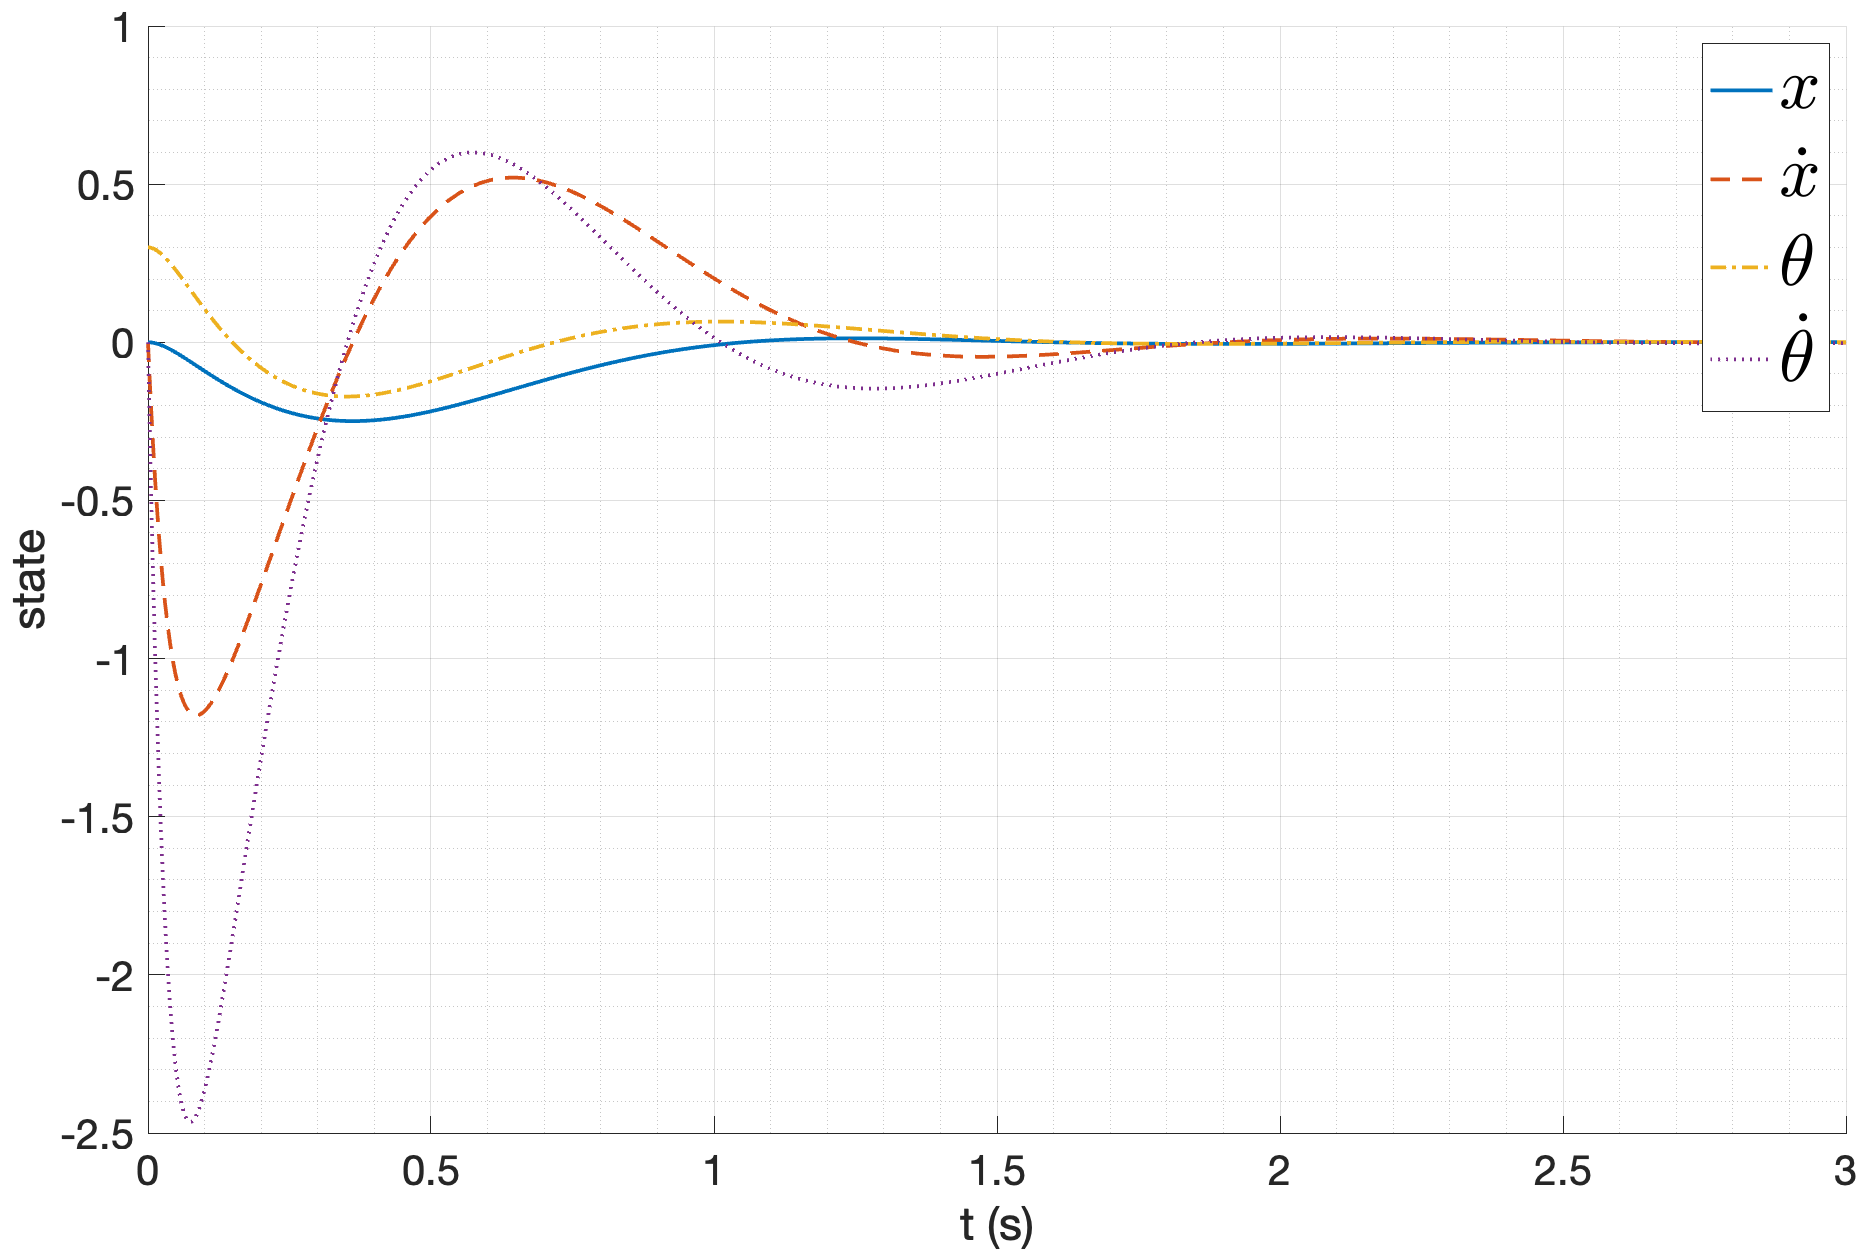
\includegraphics[width=\textwidth]{media/plots/nonmodal_control/state_1.png}
        \caption{$\theta_0 = 0.3$}
    \end{subfigure}
    \begin{subfigure}[b]{0.45\textwidth}
        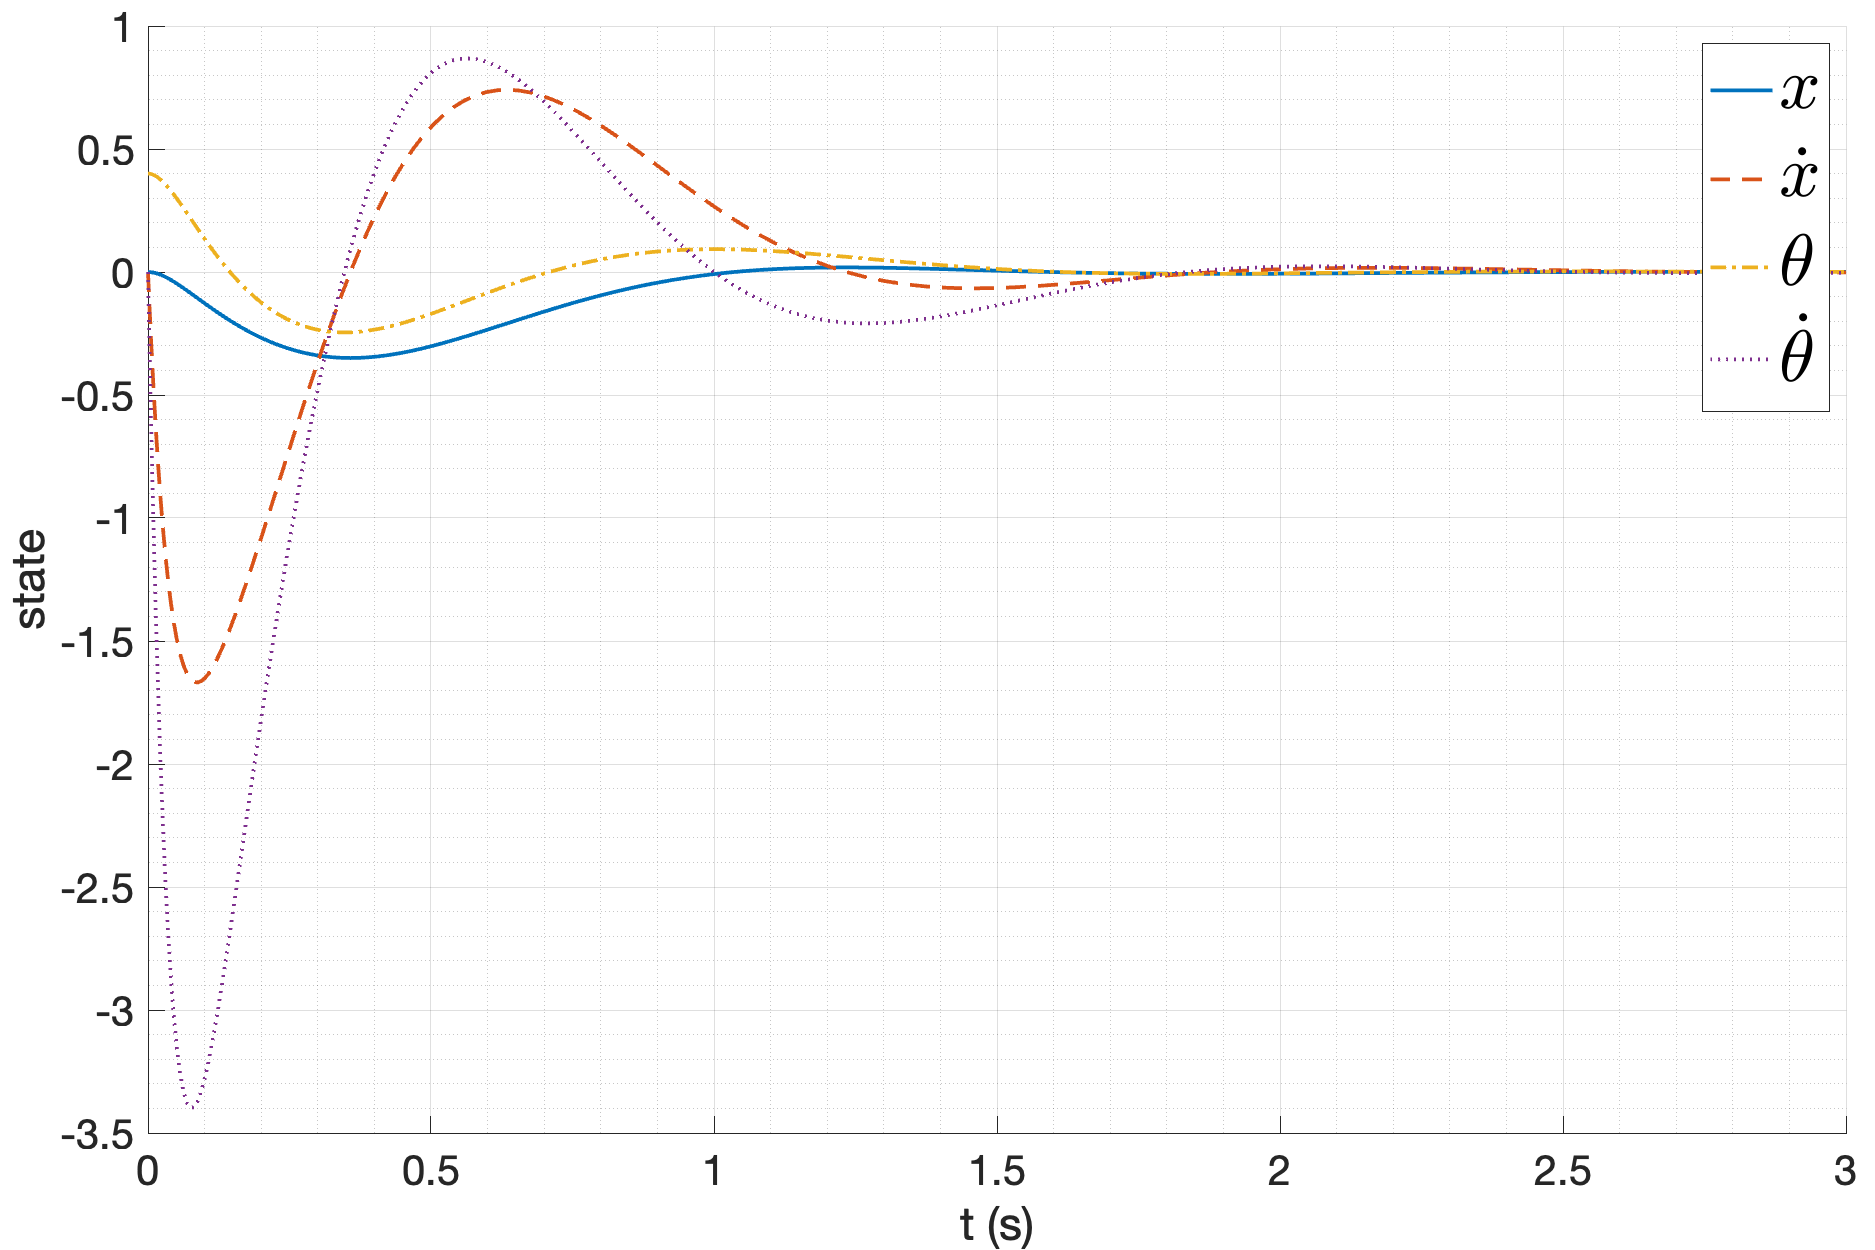
\includegraphics[width=\textwidth]{media/plots/nonmodal_control/state_2.png}
        \caption{$\theta_0 = 0.4$}
    \end{subfigure}
    \begin{subfigure}[b]{0.45\textwidth}
        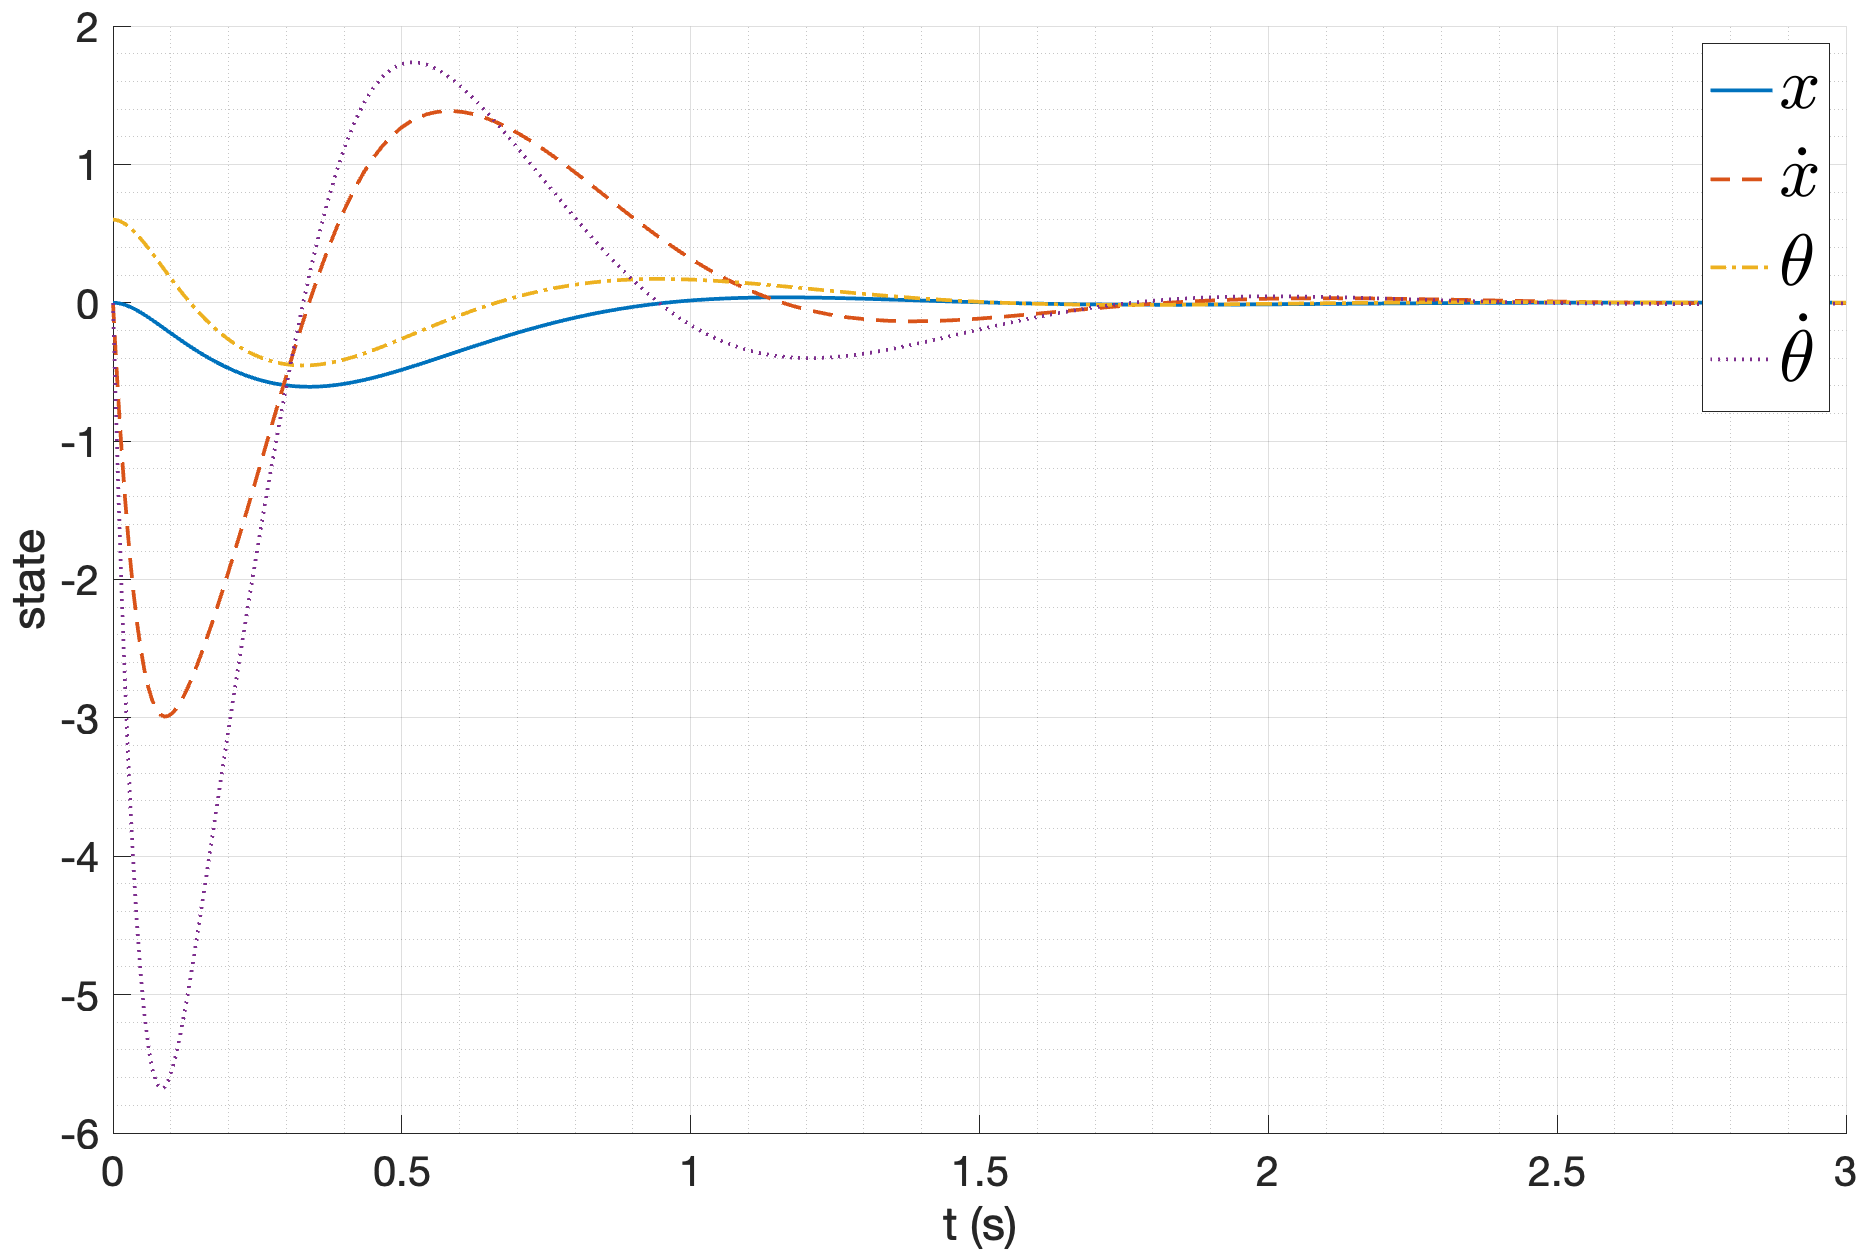
\includegraphics[width=\textwidth]{media/plots/nonmodal_control/state_3.png}
        \caption{$\theta_0 = 0.6$}
    \end{subfigure}
    \begin{subfigure}[b]{0.45\textwidth}
        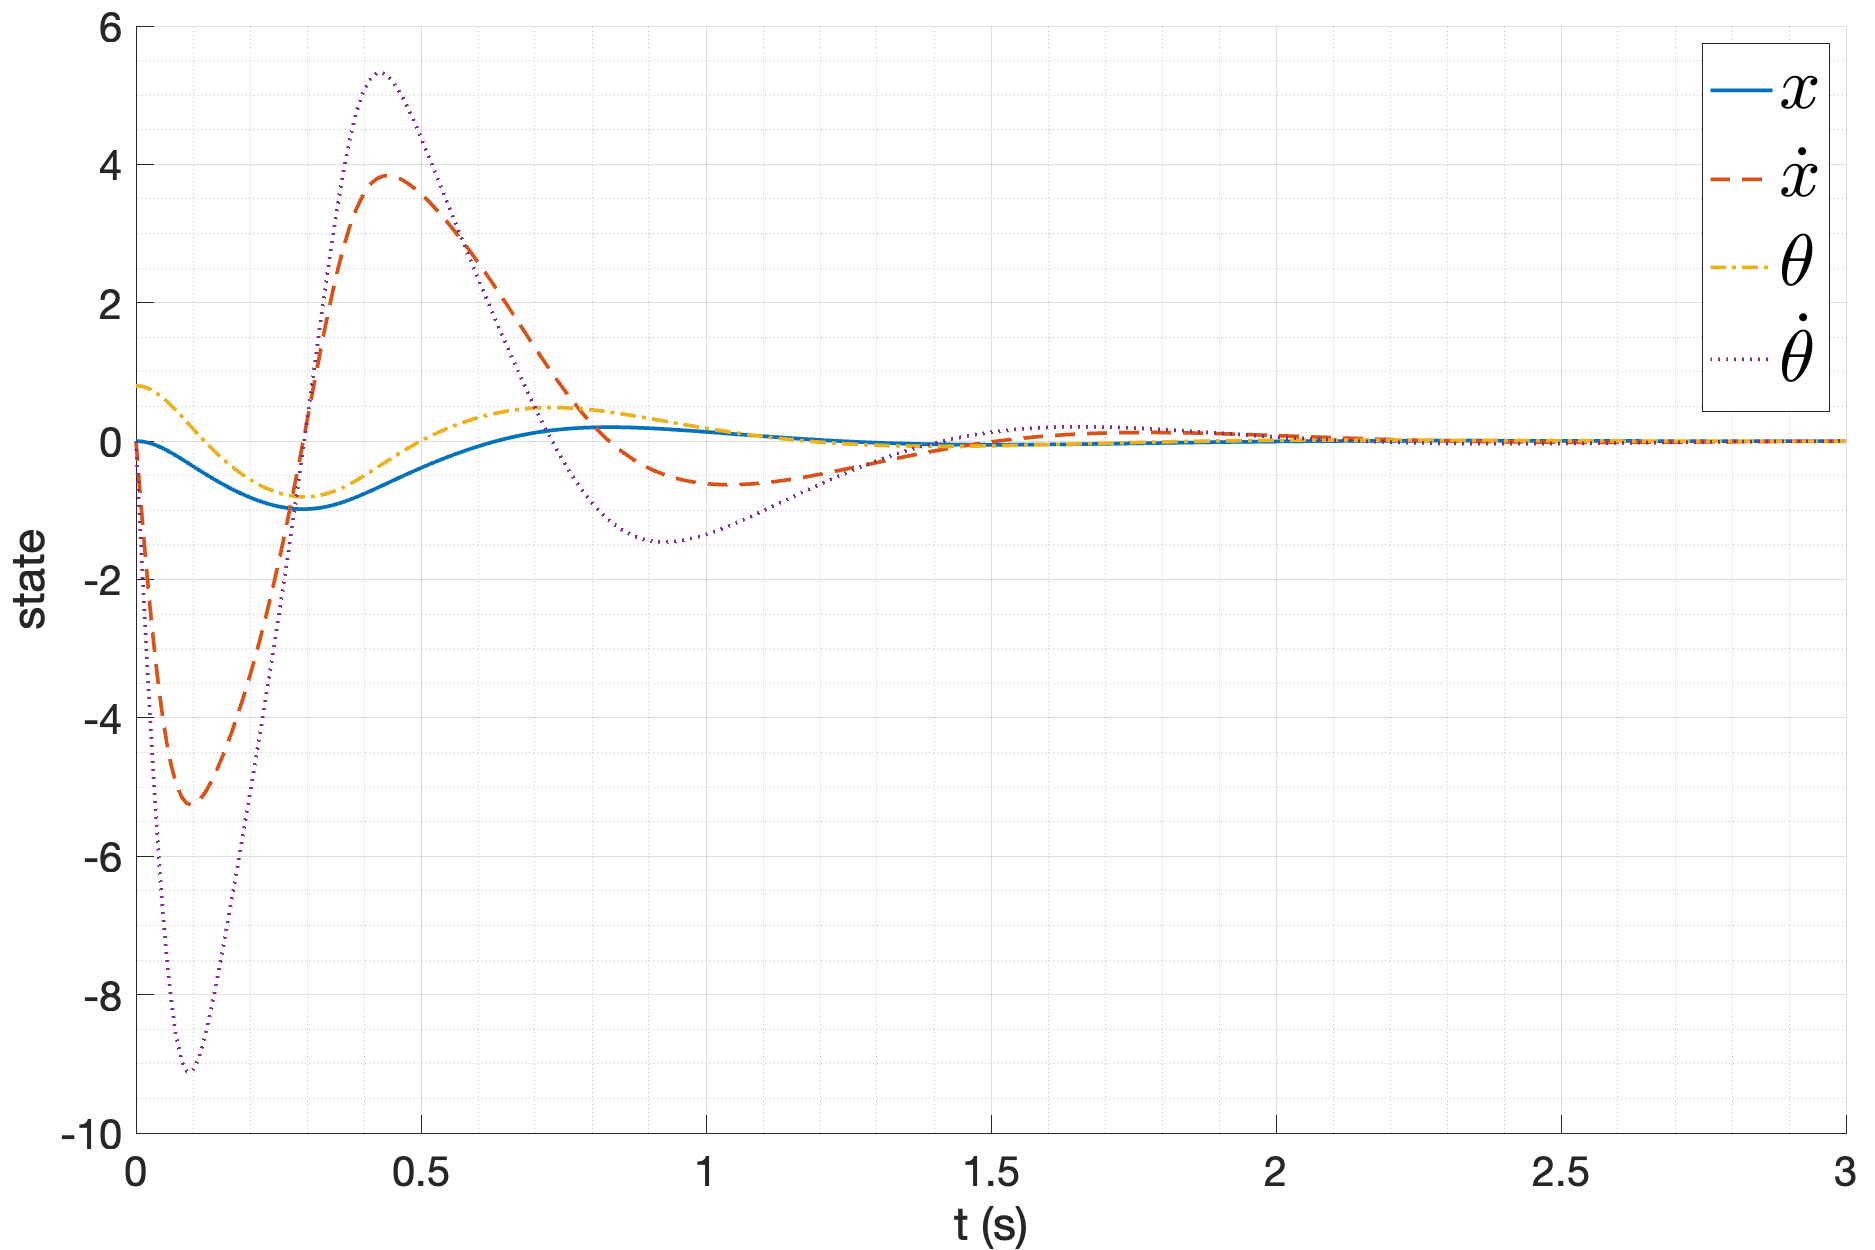
\includegraphics[width=\textwidth]{media/plots/nonmodal_control/state_4.png}
        \caption{$\theta_0 = 0.8$}
    \end{subfigure}
    \caption{Модальное управление нелинейной модели системы}
    \label{fig:nonmodal_control_initials}
\end{figure}

Также проведем моделирование при начальных условиях $x_0 = \begin{bmatrix} 0.3 & -0.2 & 0.4 & 0.6 \end{bmatrix}^T$. Результаты
моделирования приведены на рисунке \ref{fig:nonmodal_control_initials_2}.
\begin{figure}[ht!]
    \centering
    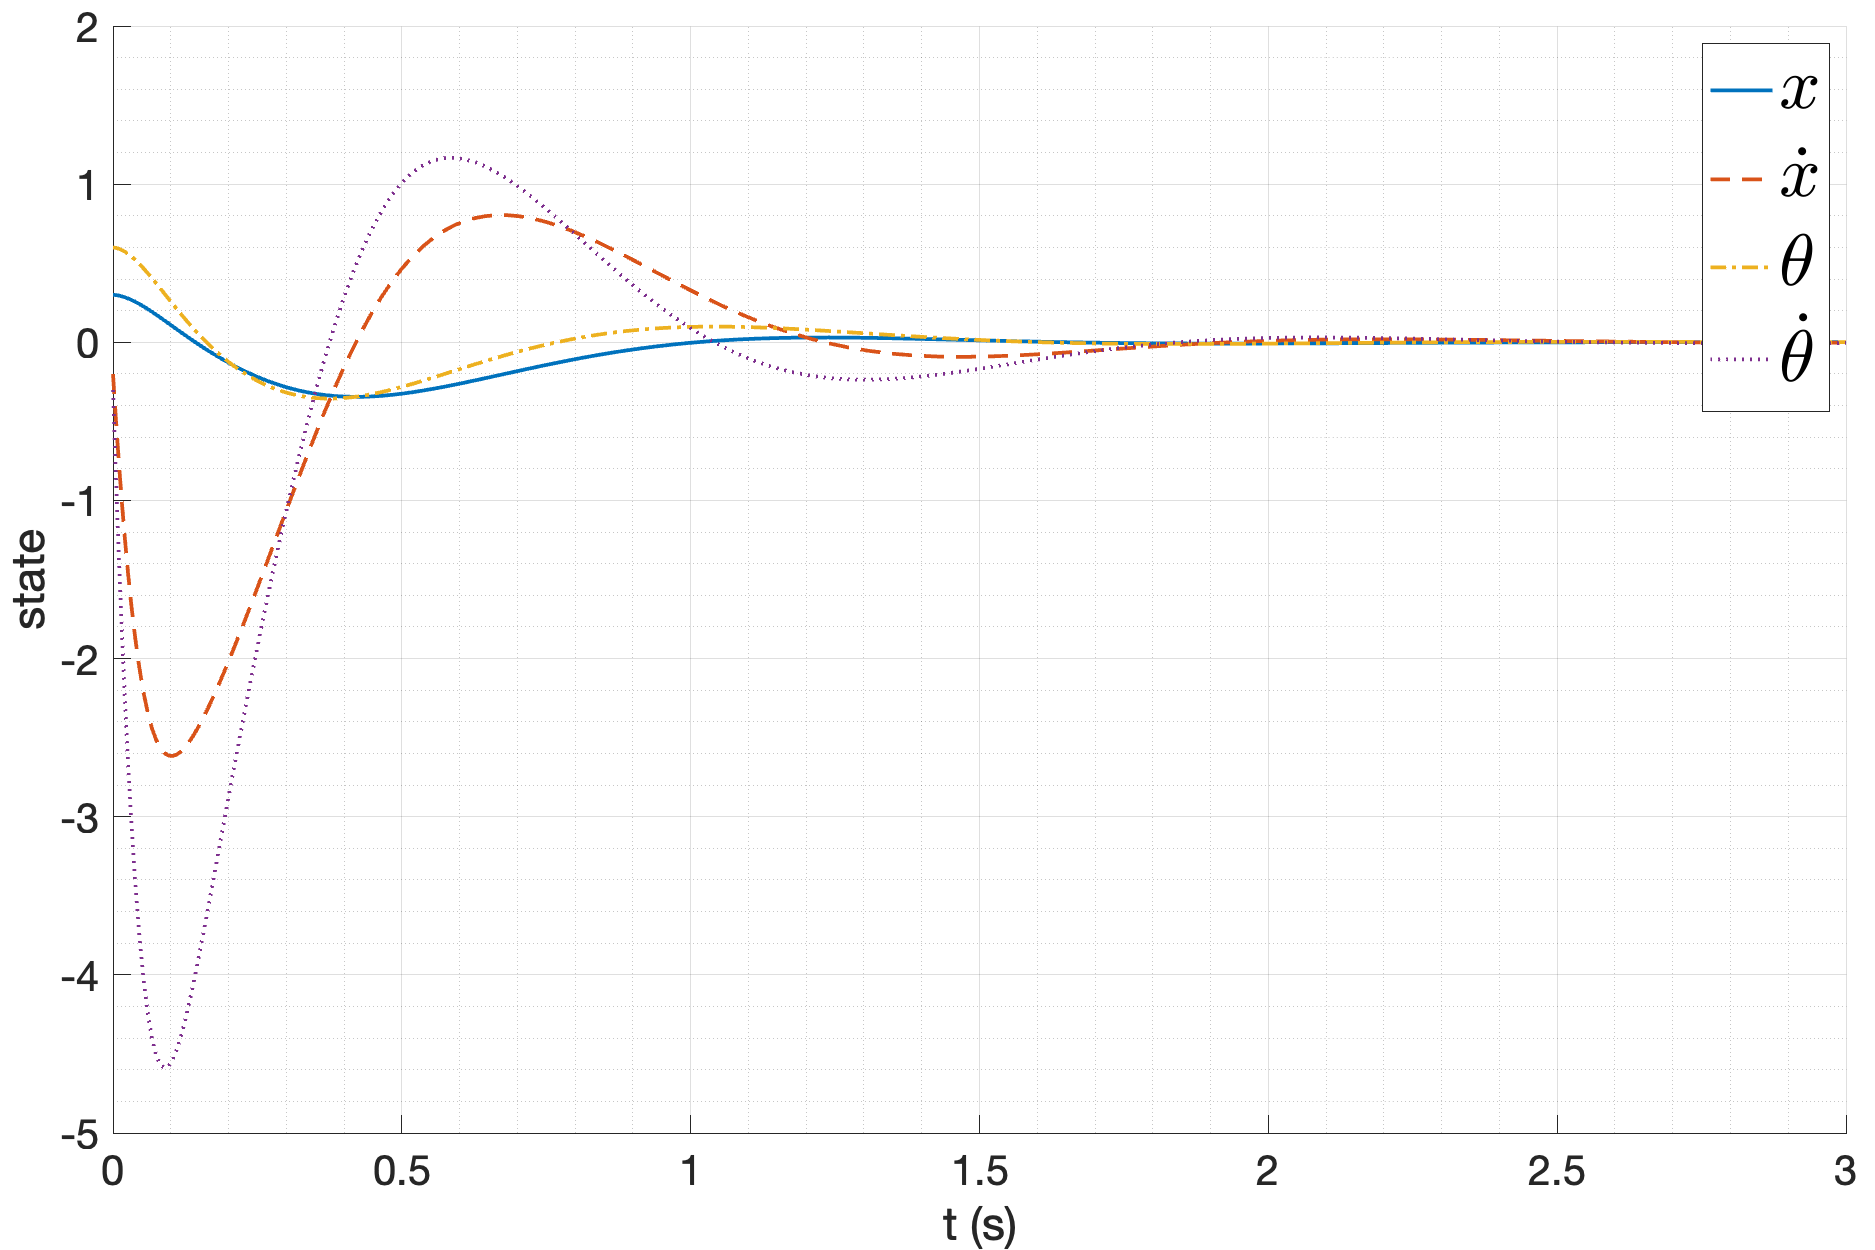
\includegraphics[width=\textwidth]{media/plots/nonmodal_control/state_5.png}
    \caption{$\theta_0 = 0.3$}
    \label{fig:nonmodal_control_initials_2}
\end{figure}
\FloatBarrier

На графиках видно, что система стабилизируется к положению равновесия при различных начальных условиях. При этом, 
чем больше начальное отклонение, тем больше требуется времени для стабилизации системы и тем больше перерегулирование. 

\subsection{Исследование переходного процесса} 
Будем рассматривать переходный процесс и управляющее воздействие при различных степенях устойчивости $\alpha$ регулятора. 
В качестве начальных условий возьмем $\theta_0 = 0.3$. В качестве степеней устойчивости будем использовать 
значения $\alpha \in \begin{bmatrix} 1, 3, 6\end{bmatrix}$. Для каждого значения $\alpha$ будем 
синтезировать регулятор и исследовать его влияние на переходный процесс. 

Полученные регуляторы: 
\begin{enumerate}
    \item $\alpha = 1$: $K = \begin{bmatrix} 2180.49  & 2549.34  & -11475.12  & -2606.25 \\ \end{bmatrix}$, $\sigma(A + BK) = \begin{bmatrix} -2.12 + 5.02j \\ -2.12 - 5.02j \\ -4.35 \\ -1.26 \\  \end{bmatrix}$
    \item \item $\alpha = 3$: $K = \begin{bmatrix} 18189.83  & 11279.39  & -35086.93  & -8004.31 \\ \end{bmatrix}$, $\sigma(A + BK) = \begin{bmatrix} -4.52 + 8.36j \\ -4.52 - 8.36j \\ -4.34 \\ -3.46 \\  \end{bmatrix}$
    \item $\alpha = 6$: $K = \begin{bmatrix} 230529.7  & 76168.3  & -208685.7  & -43384.3 \\ \end{bmatrix}$, $\sigma(A + BK) = \begin{bmatrix} -9.84 + 16.2j \\ -9.84 - 16.2j \\ -6.55 + 2.1j \\ -6.55 - 2.1j \\ \end{bmatrix}$
\end{enumerate}
Все регуляторы синтезировались корректно, устойчивость каждой системы соответствует заданной степени устойчивости $\alpha$. 

Проведем моделирование переходного процесса для каждого из полученных регуляторов. 

Результаты моделирования приведены на рисунках \ref{fig:nonmodal_control_alpha_1} - \ref{fig:nonmodal_control_alpha_3_u}.
Сравнительные графики переходных процессов приведены на рисунке \ref{fig:nonmodal_control_cmp_x} и \ref{fig:nonmodal_control_cmp_ang}.

\begin{figure}[ht!]
    \centering
    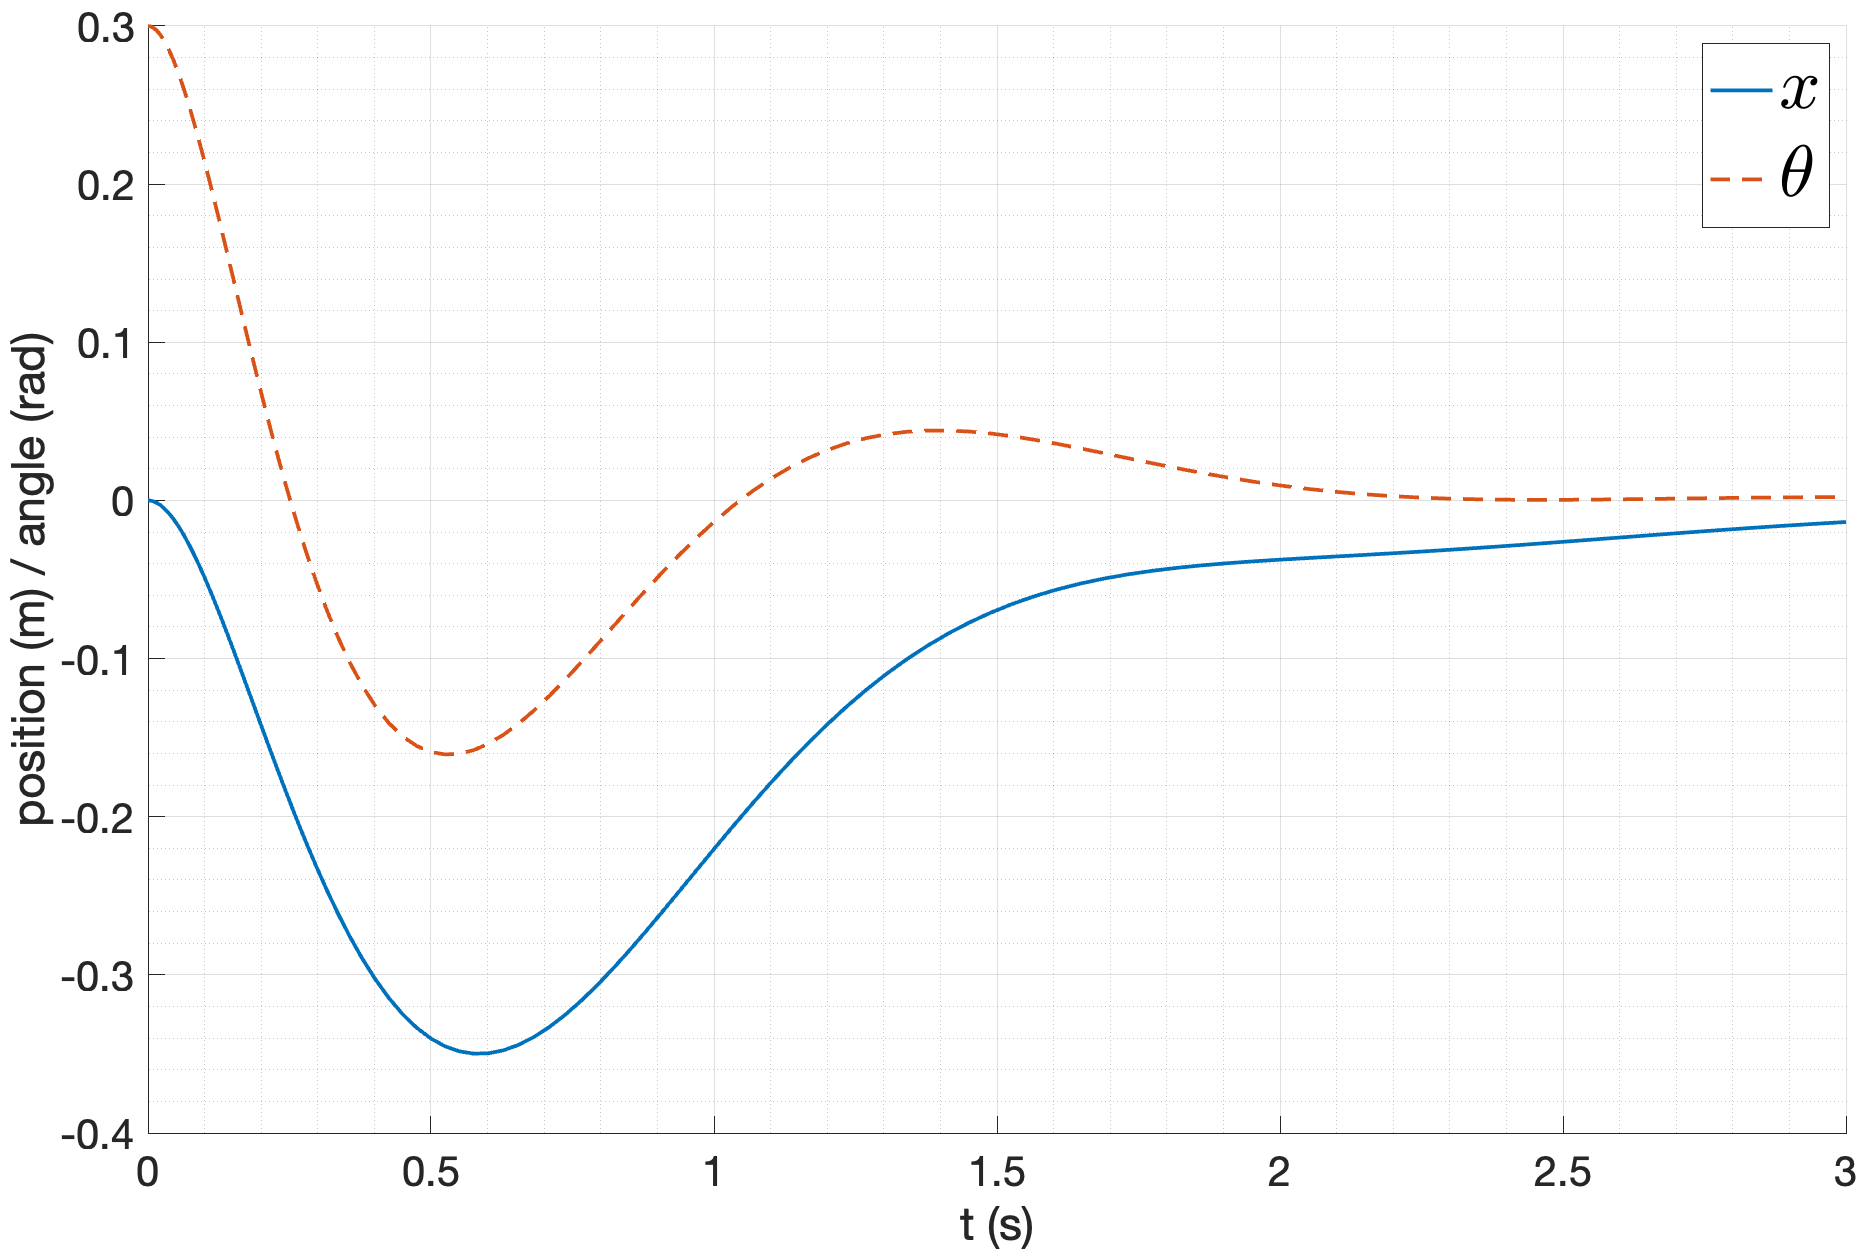
\includegraphics[width=\textwidth]{media/plots/nonmodal_controllers/out_1.png}
    \caption{Выход системы при $\alpha = 1$}
    \label{fig:nonmodal_control_alpha_1}
\end{figure}
\begin{figure}
    \centering
    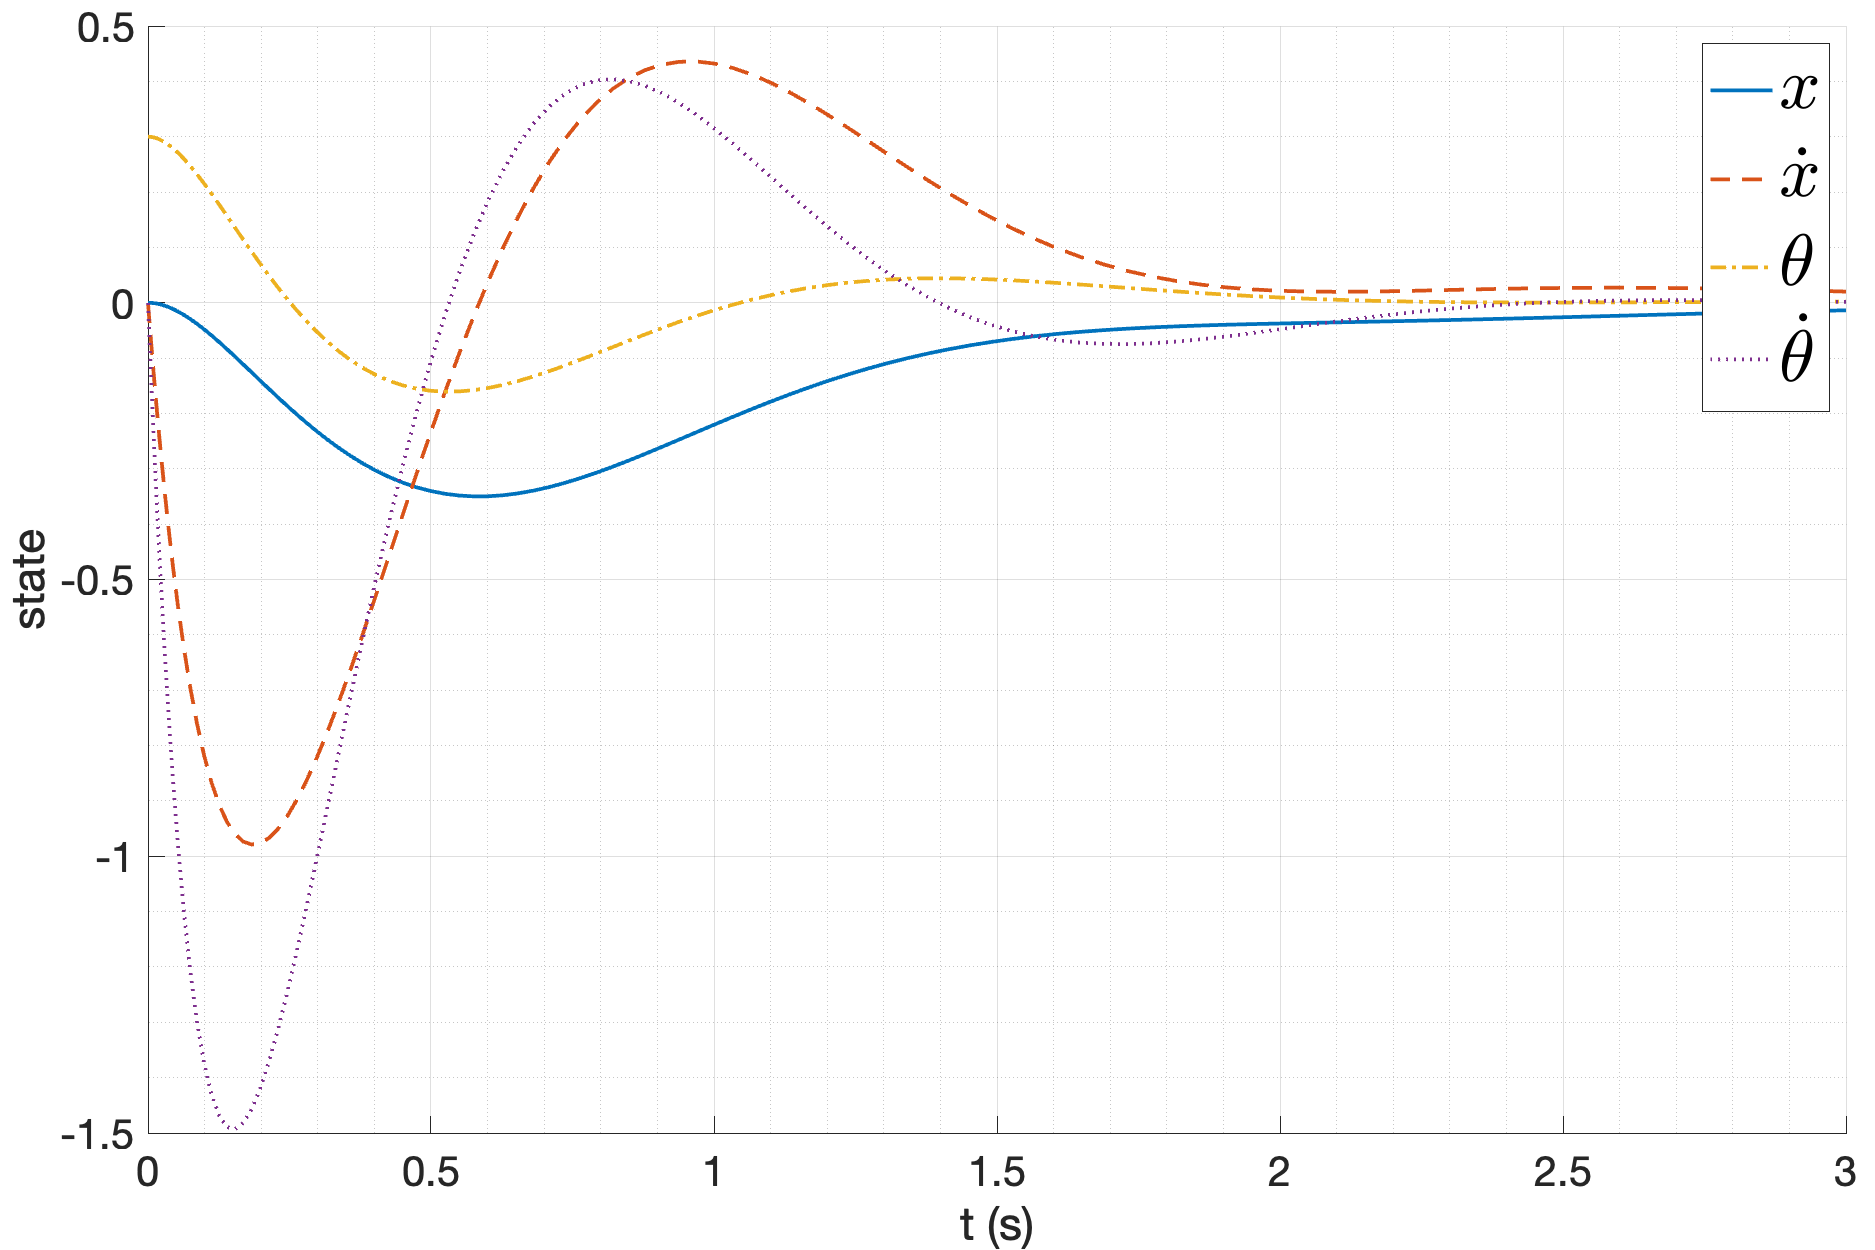
\includegraphics[width=\textwidth]{media/plots/nonmodal_controllers/state_1.png}
    \caption{Вектор состояния при $\alpha = 1$}
    \label{fig:nonmodal_control_alpha_1_u}
\end{figure}
\begin{figure}[ht!]
    \centering
    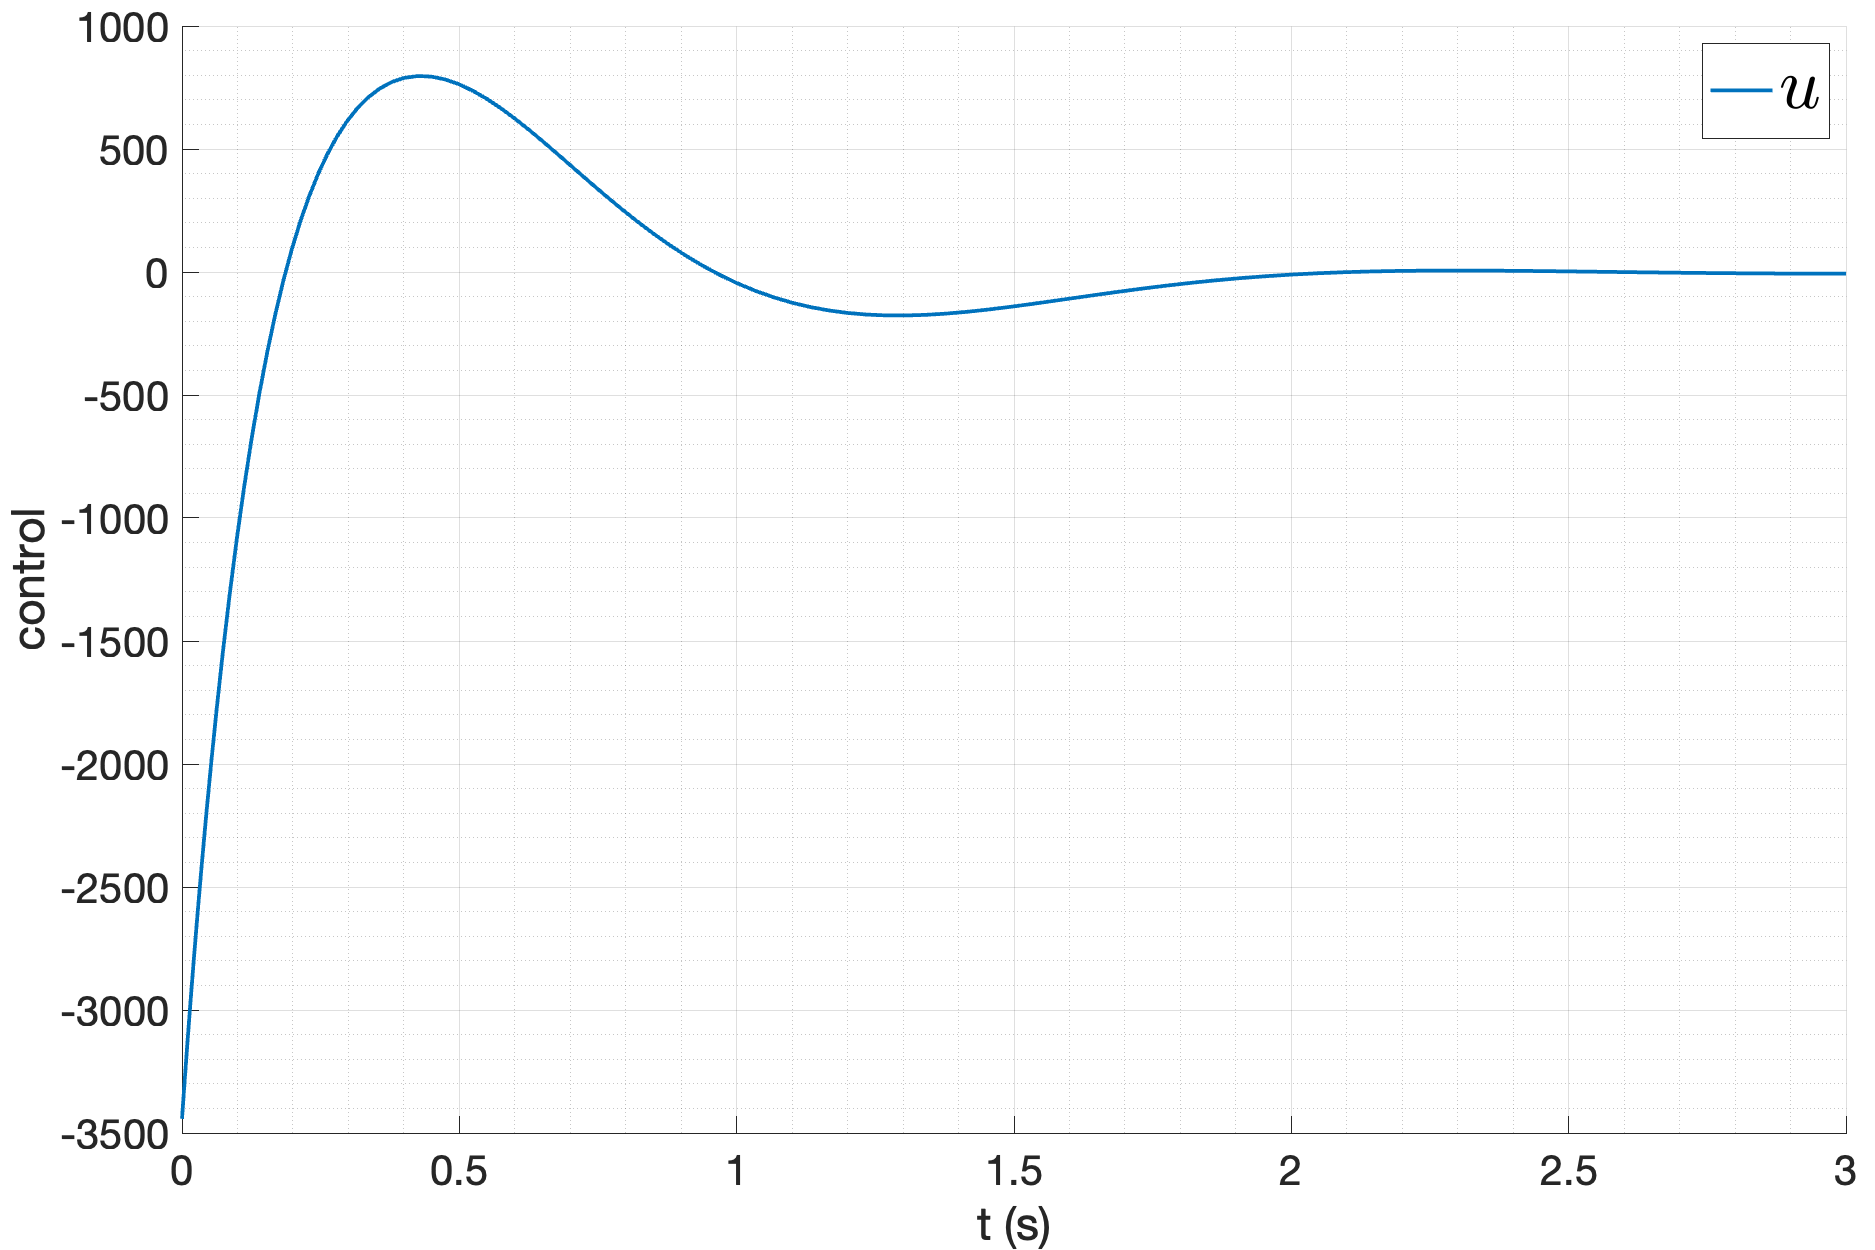
\includegraphics[width=\textwidth]{media/plots/nonmodal_controllers/u_1.png}
    \caption{Управляющее воздействие при $\alpha = 1$}
    \label{fig:nonmodal_control_alpha_1_u}
\end{figure}
\begin{figure}[ht!]
    \centering
    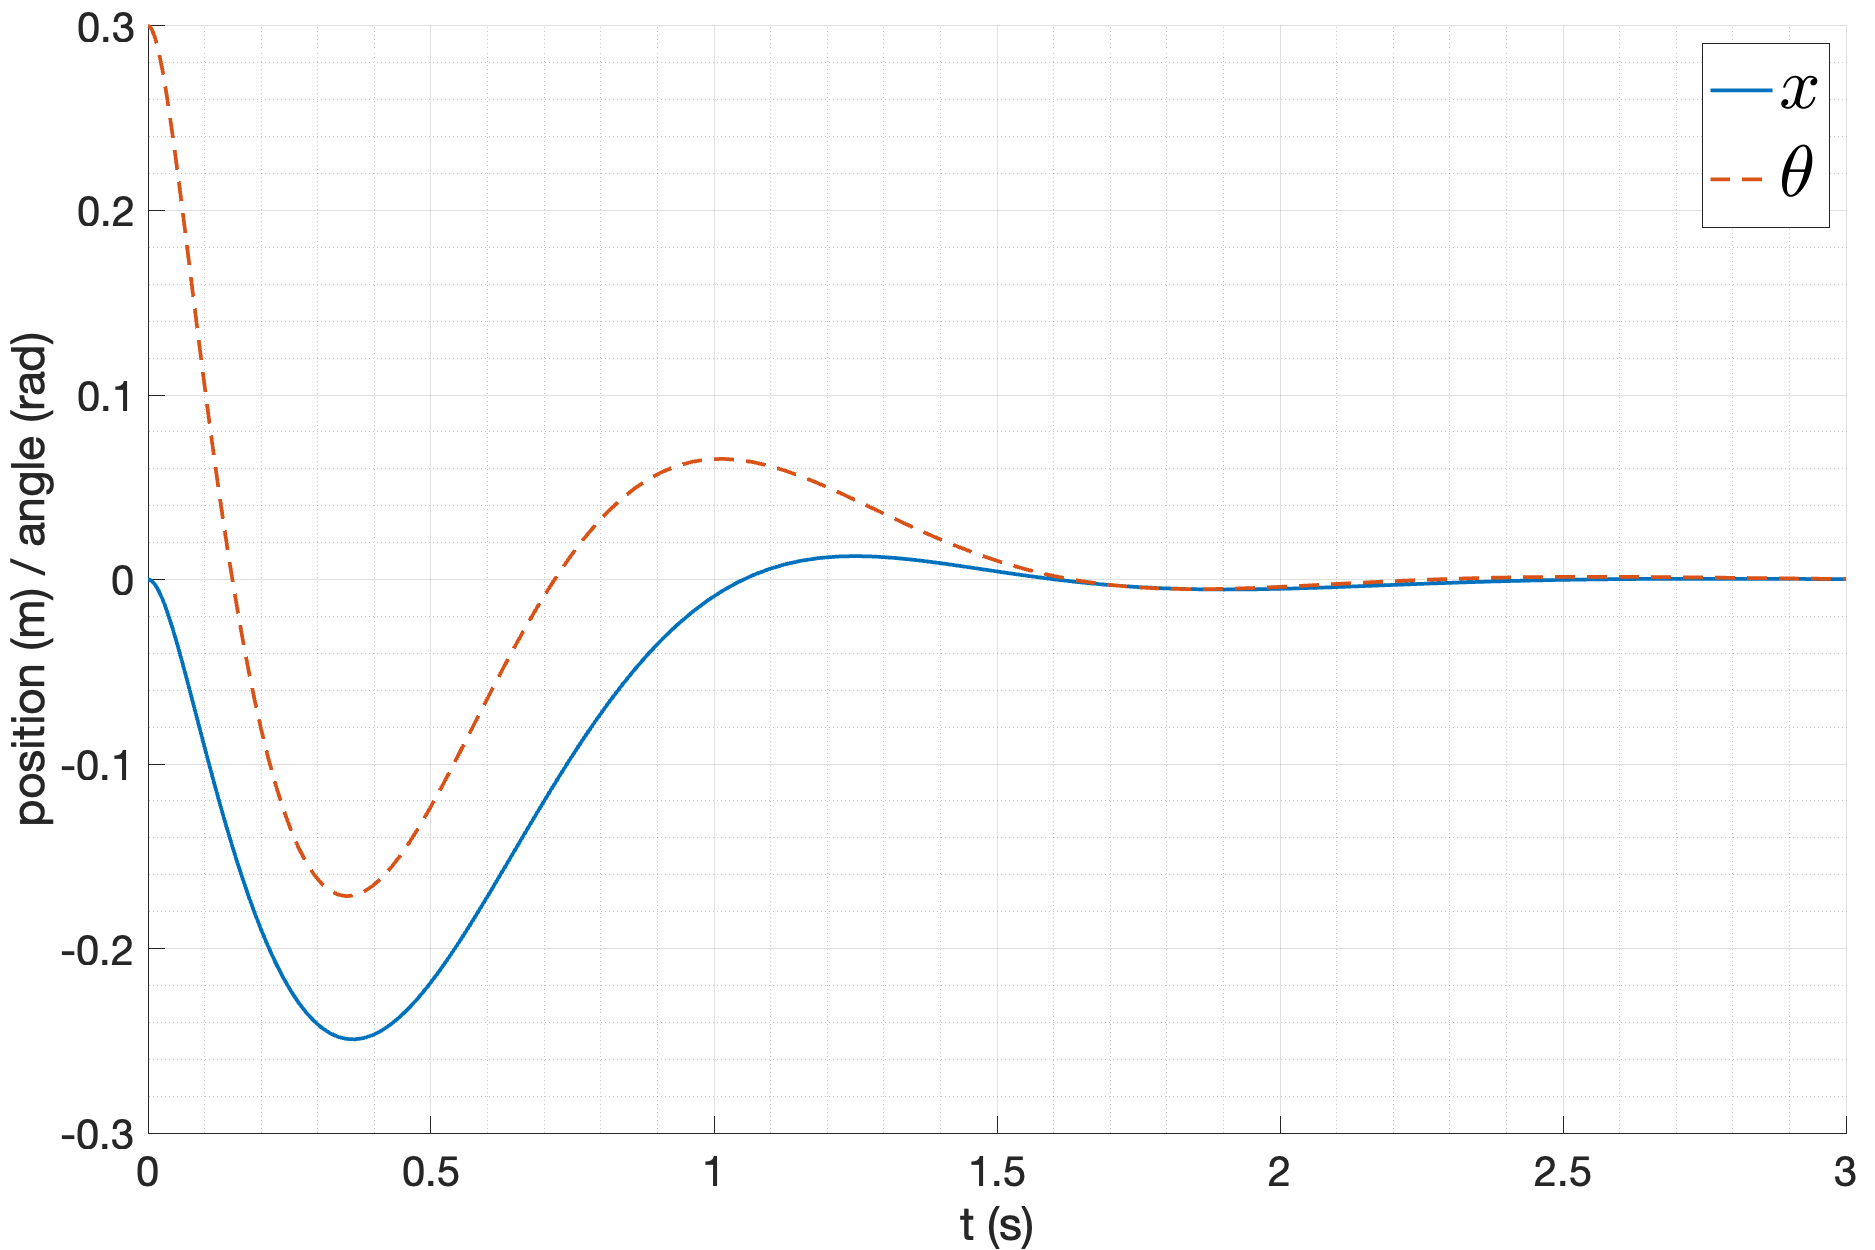
\includegraphics[width=\textwidth]{media/plots/nonmodal_controllers/out_2.png}
    \caption{Выход системы при $\alpha = 3$}
    \label{fig:nonmodal_control_alpha_2}
\end{figure}
\begin{figure}[ht!]
    \centering
    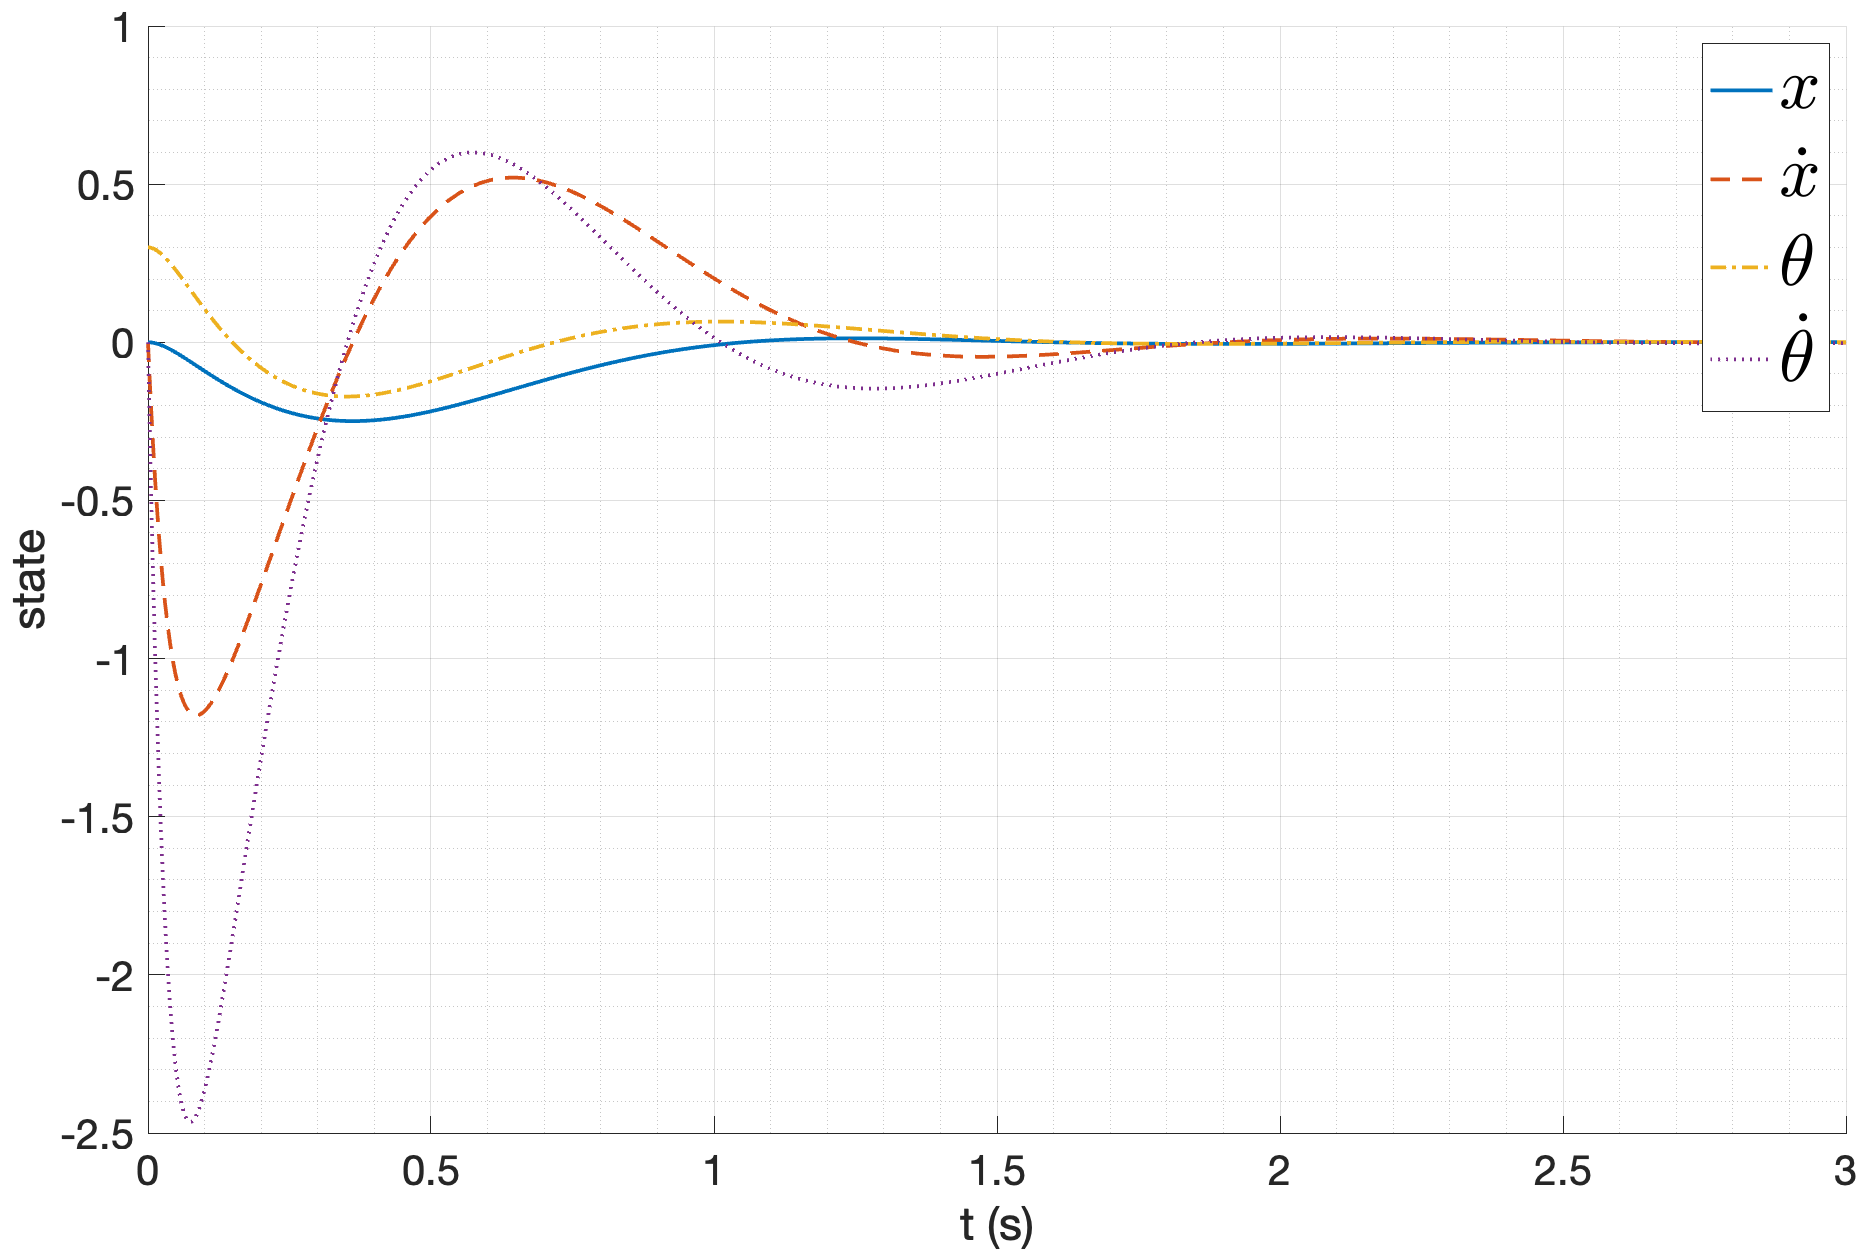
\includegraphics[width=\textwidth]{media/plots/nonmodal_controllers/state_2.png}
    \caption{Вектор состояния при $\alpha = 3$}
    \label{fig:nonmodal_control_alpha_2_u}
\end{figure}
\begin{figure}[ht!]
    \centering
    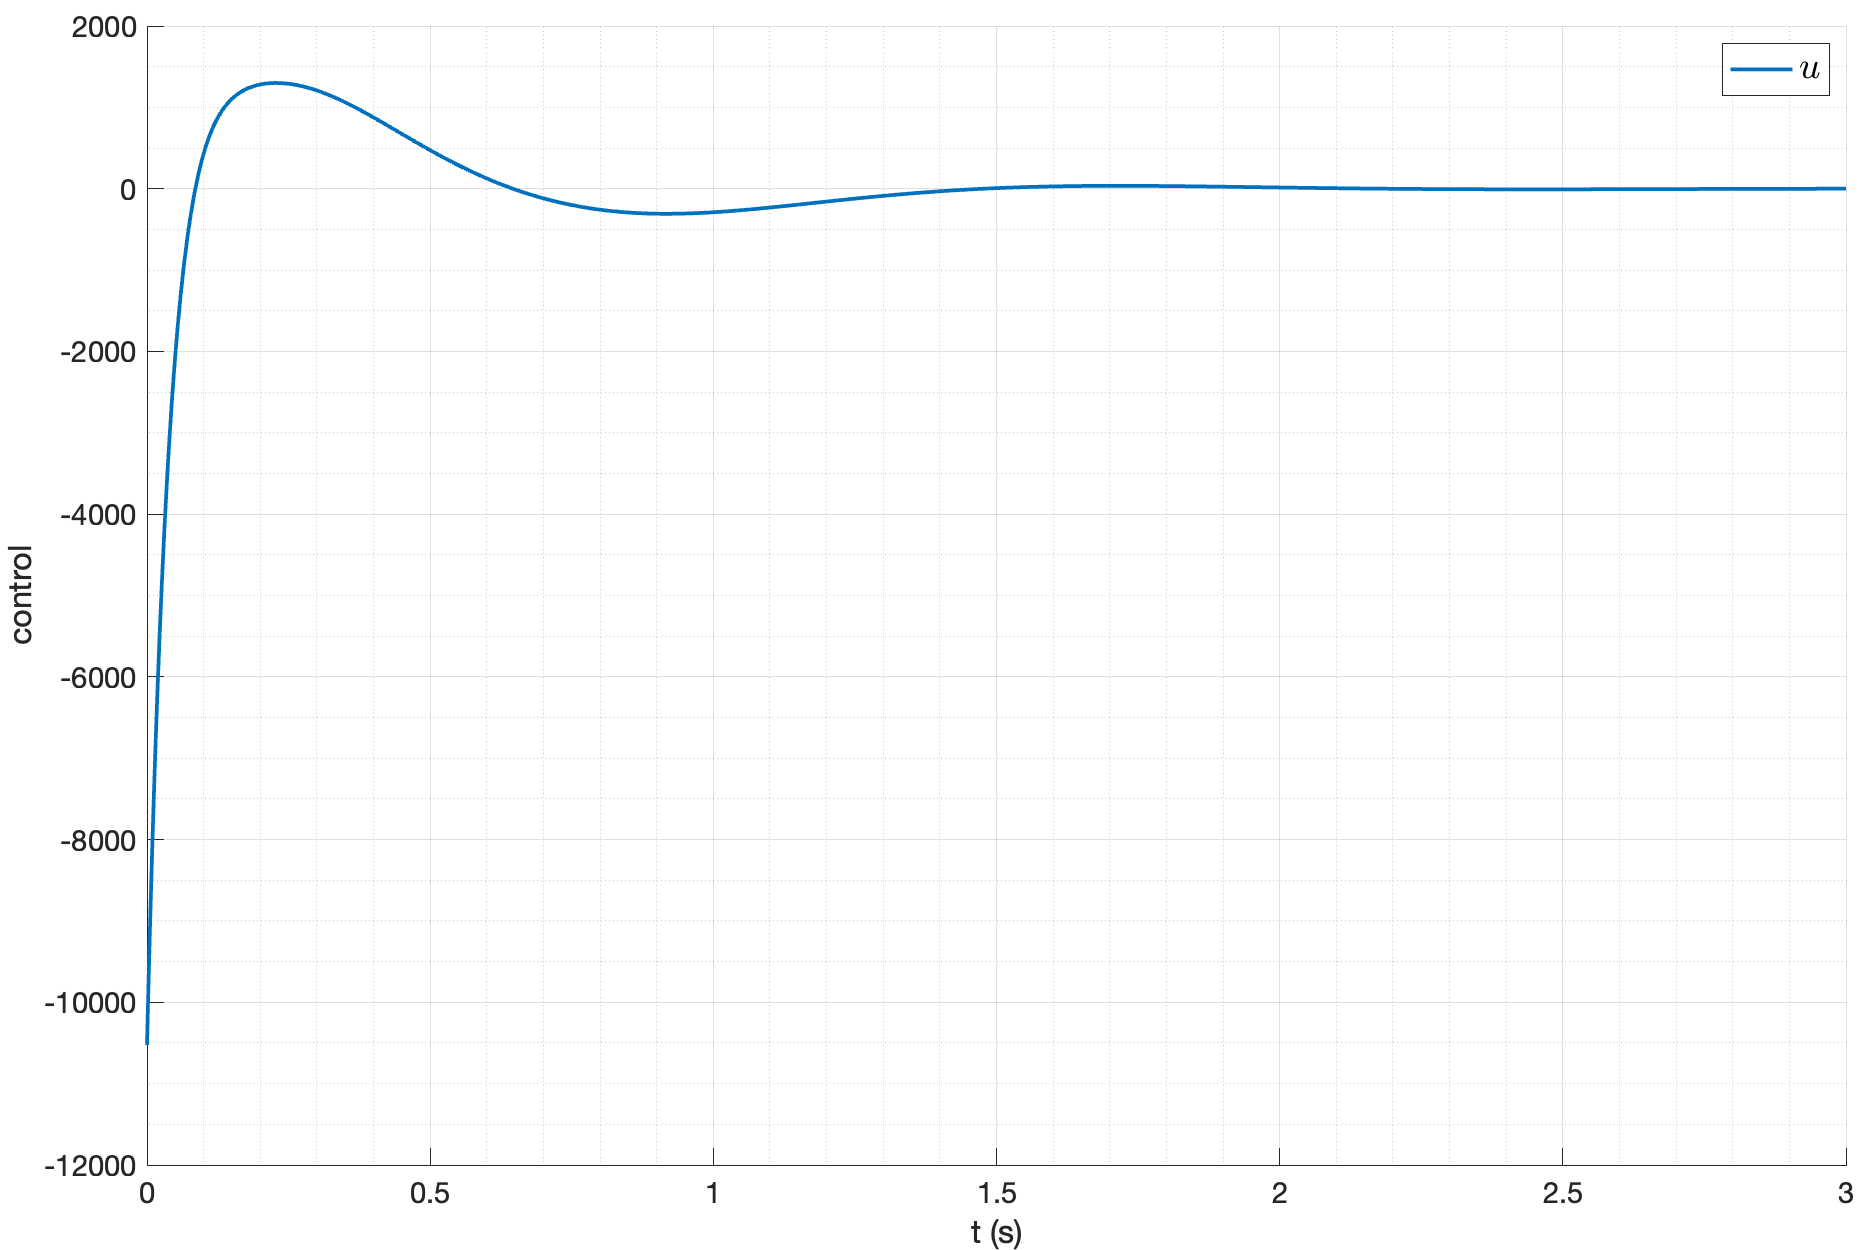
\includegraphics[width=\textwidth]{media/plots/nonmodal_controllers/u_2.png}
    \caption{Управляющее воздействие при $\alpha = 3$}
    \label{fig:nonmodal_control_alpha_2_u}
\end{figure}
\begin{figure}[ht!]
    \centering
    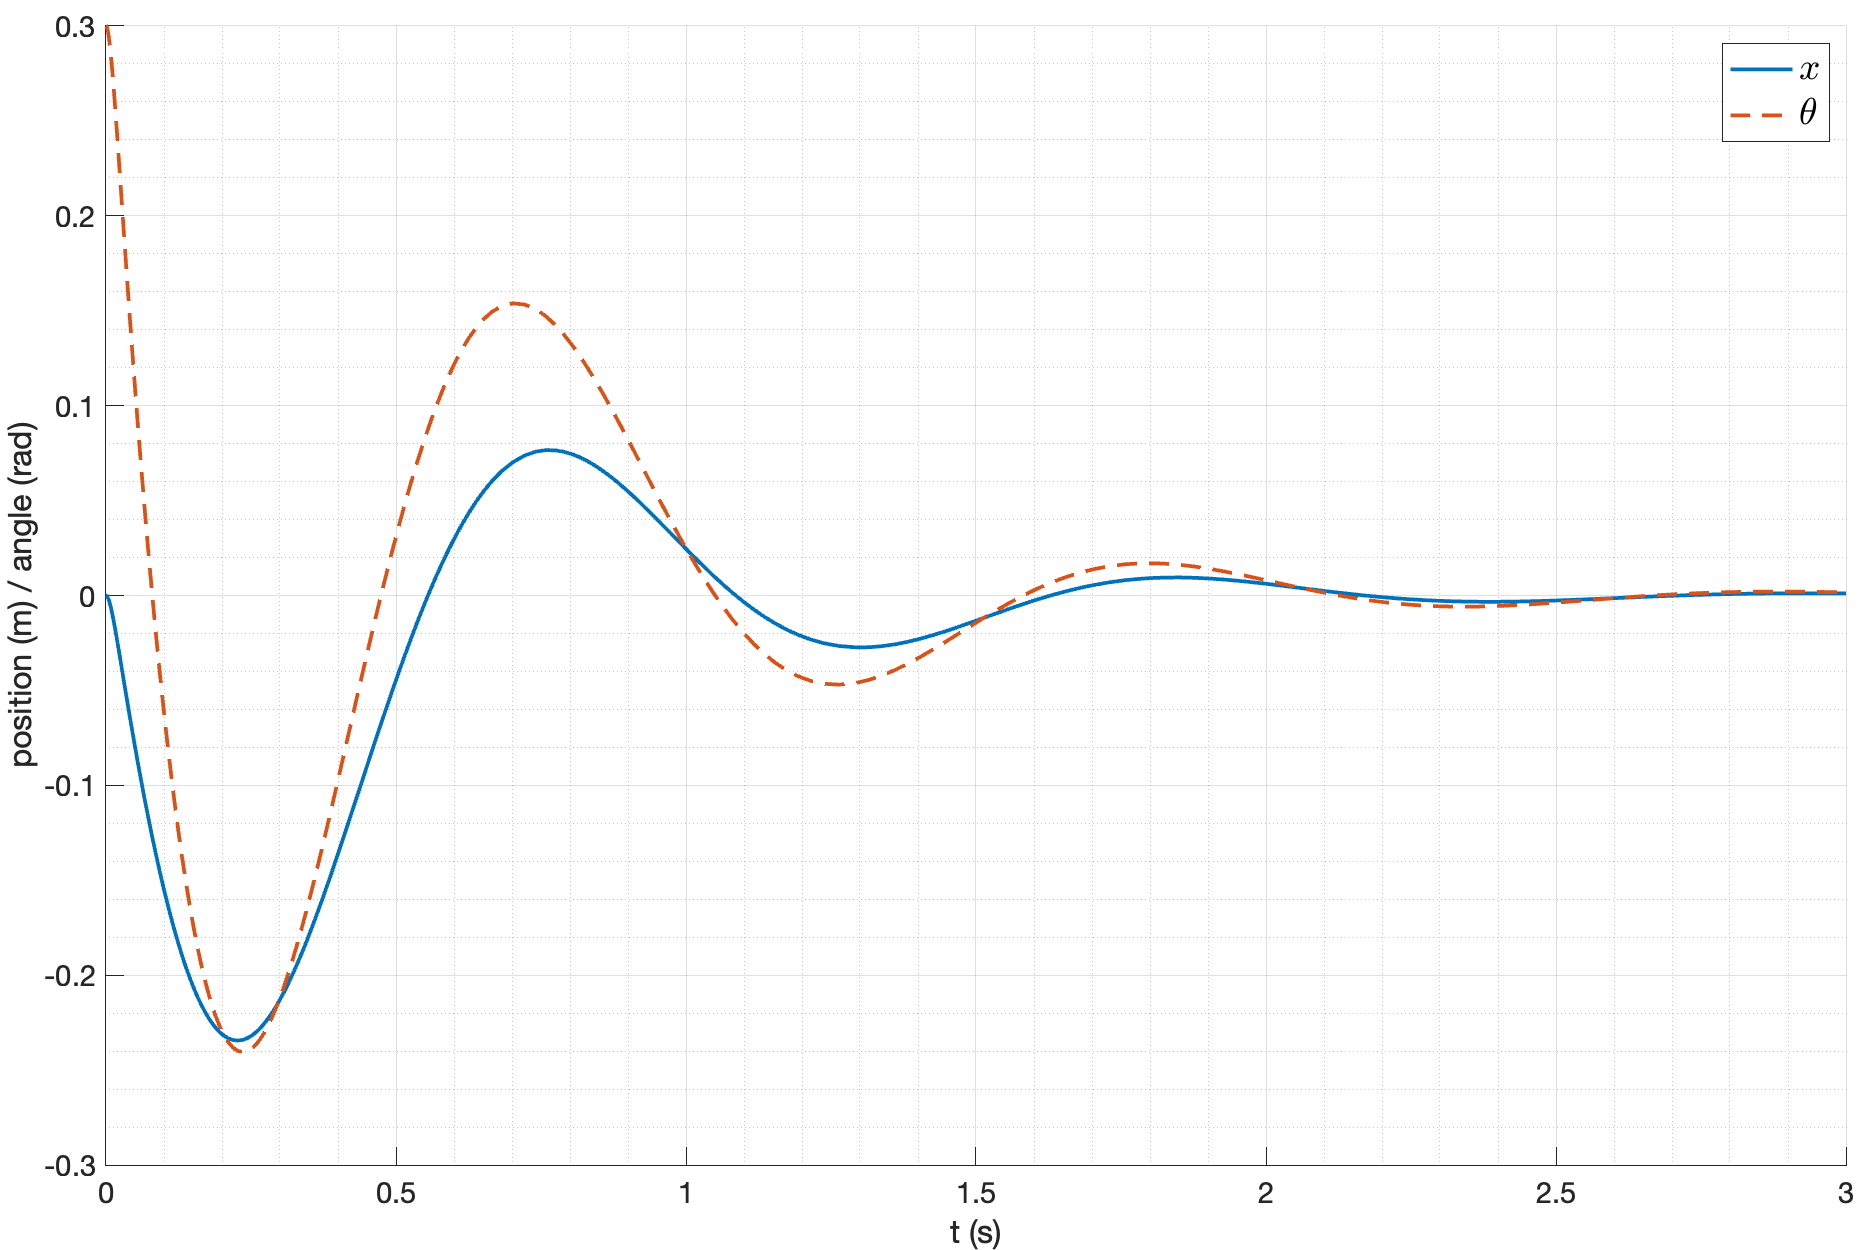
\includegraphics[width=\textwidth]{media/plots/nonmodal_controllers/out_3.png}
    \caption{Выход системы при $\alpha = 6$}
    \label{fig:nonmodal_control_alpha_3}
\end{figure}
\begin{figure}[ht!]
    \centering
    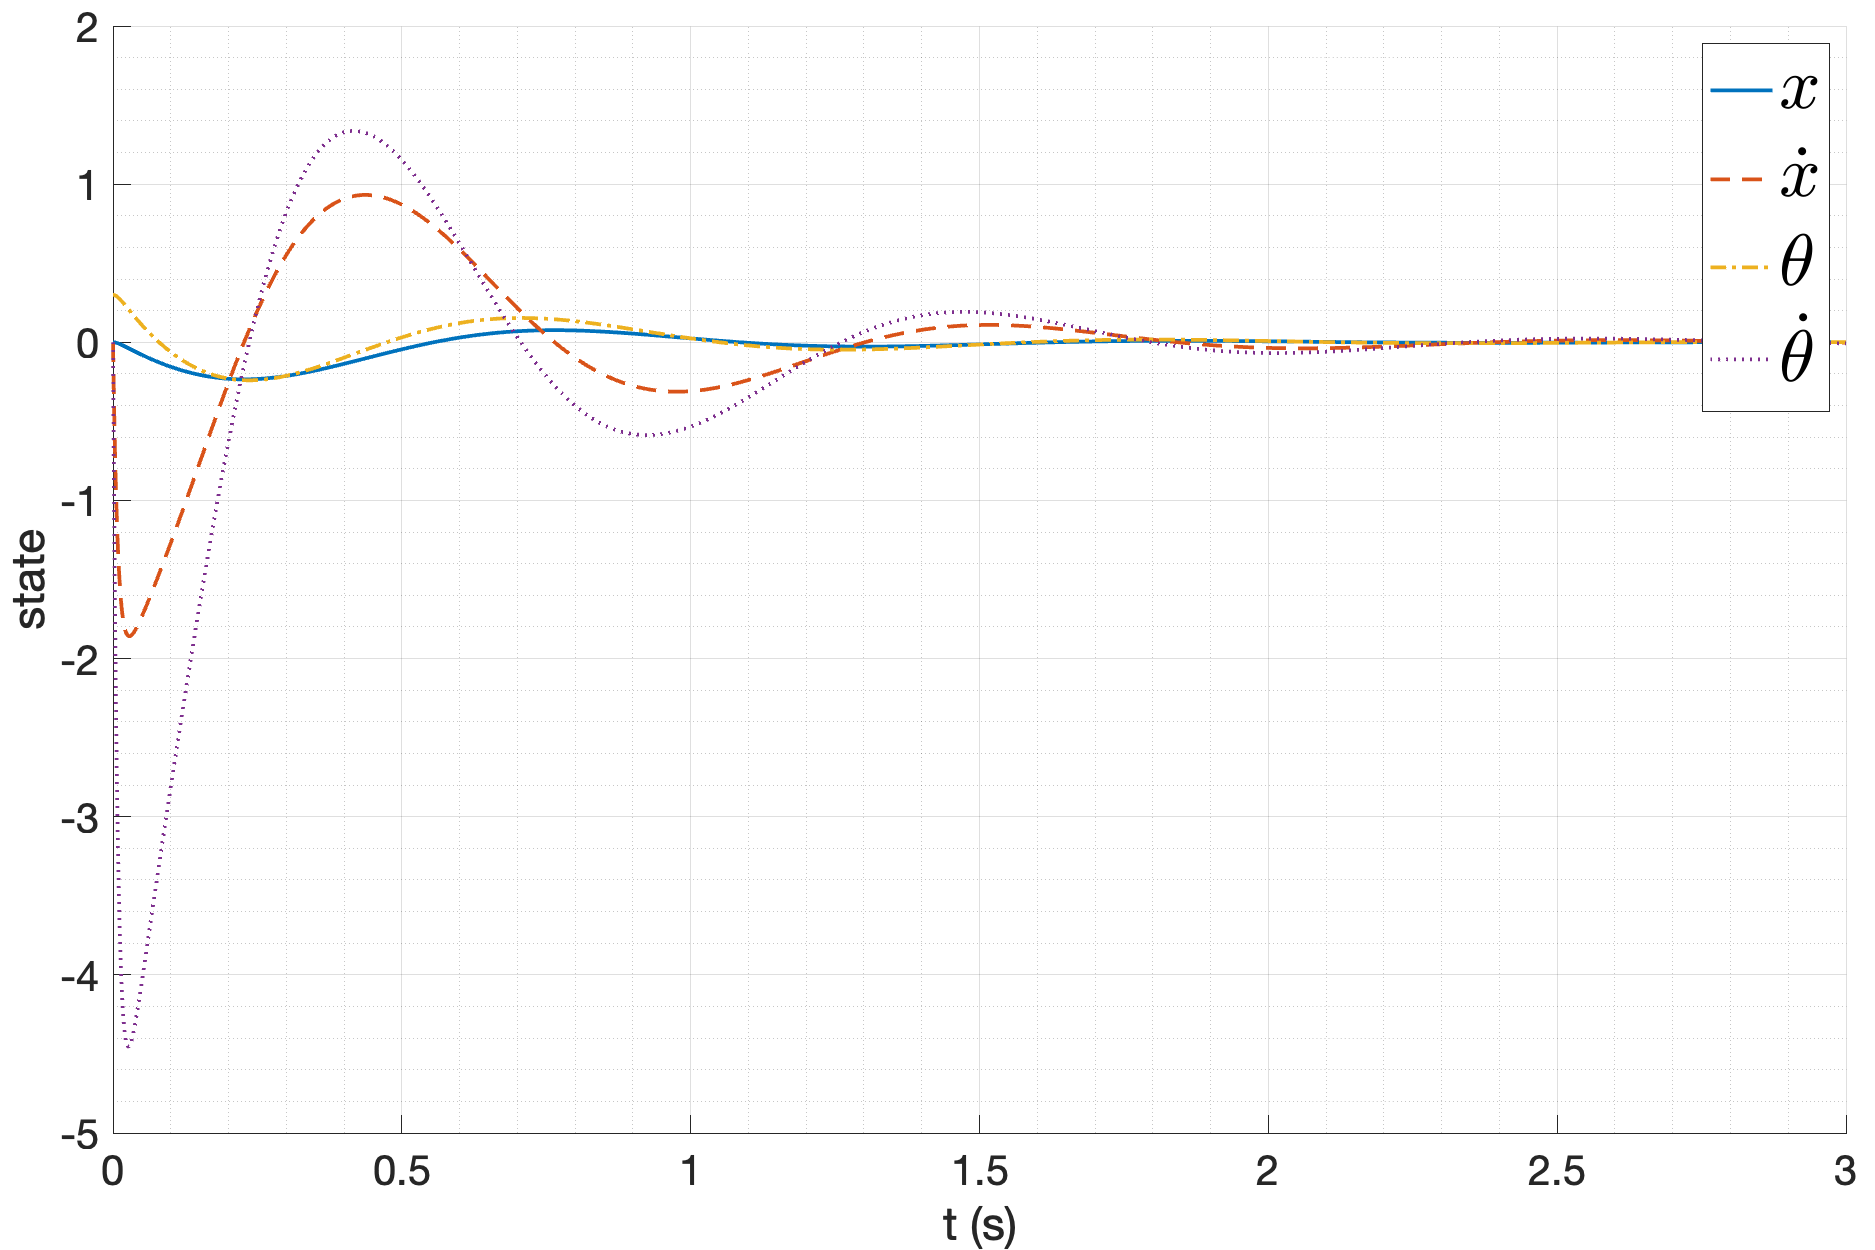
\includegraphics[width=\textwidth]{media/plots/nonmodal_controllers/state_3.png}
    \caption{Вектор состояния при $\alpha = 6$}
    \label{fig:nonmodal_control_alpha_3_u}
\end{figure}
\begin{figure}[ht!]
    \centering
    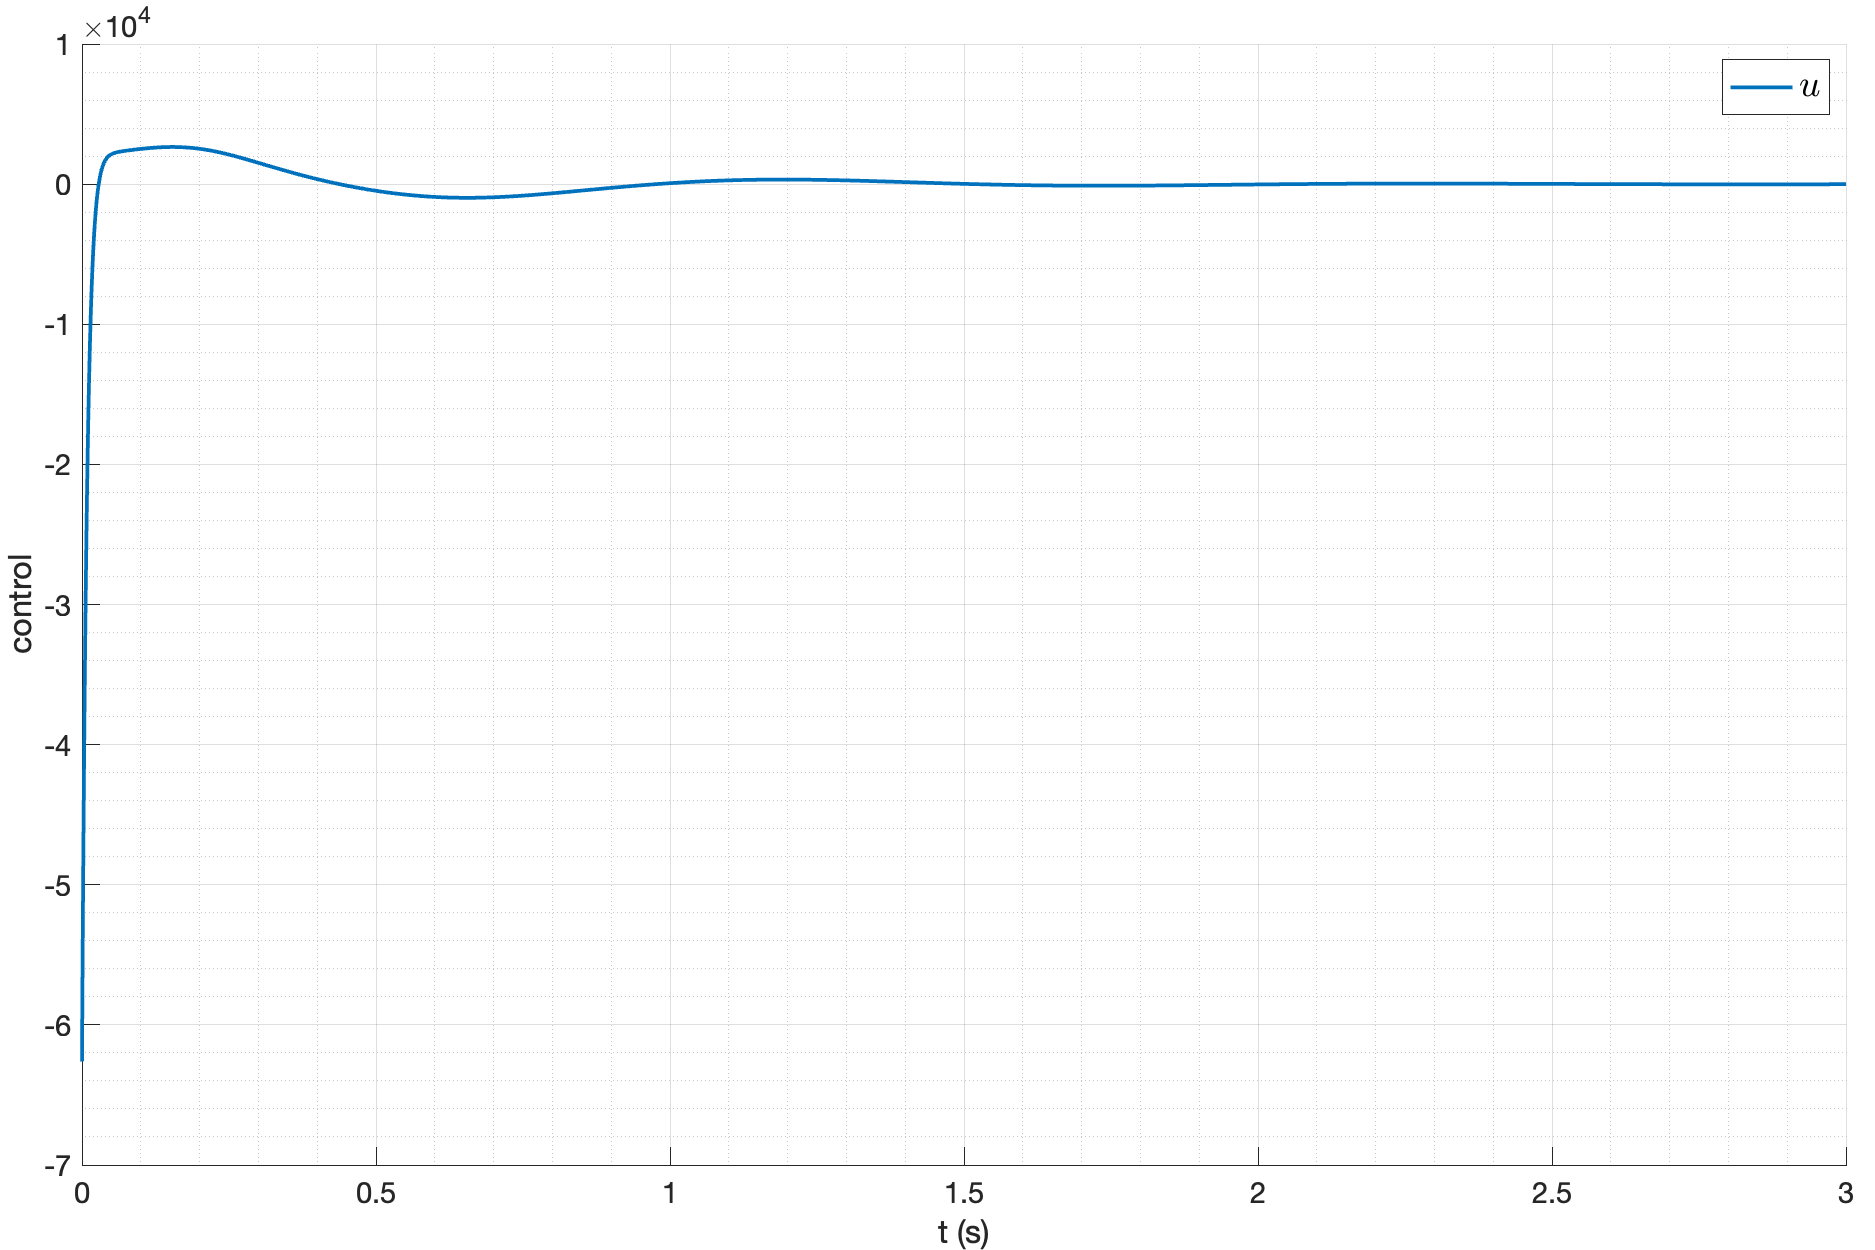
\includegraphics[width=\textwidth]{media/plots/nonmodal_controllers/u_3.png}
    \caption{Управляющее воздействие при $\alpha = 6$}
    \label{fig:nonmodal_control_alpha_3_u}
\end{figure}

\begin{figure}[ht!]
    \centering
    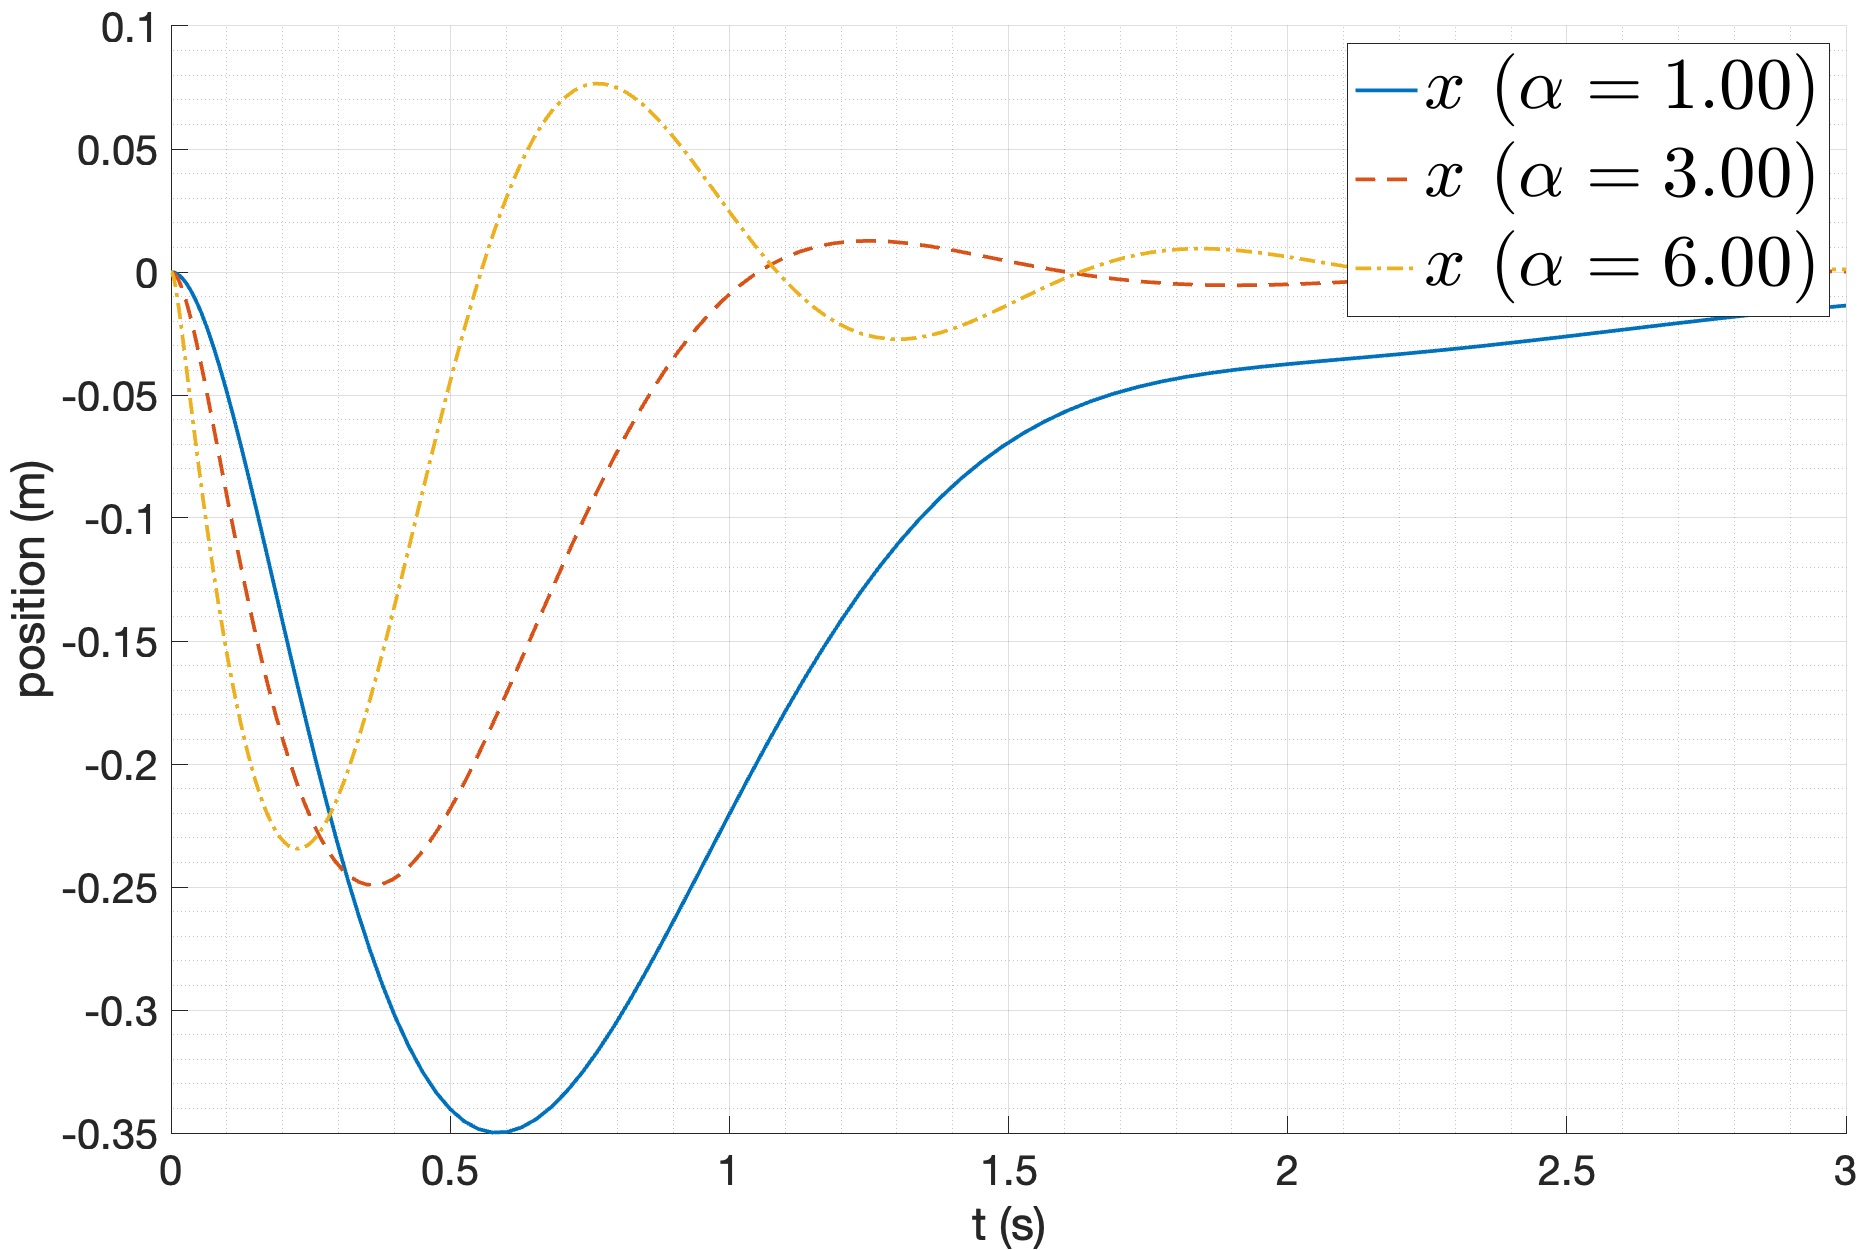
\includegraphics[width=\textwidth]{media/plots/nonmodal_controllers/x_cmp.png}
    \caption{Сравнение переходных процессов по смещению тележки}
    \label{fig:nonmodal_control_cmp_x}
\end{figure}
\begin{figure}[ht!]
    \centering
    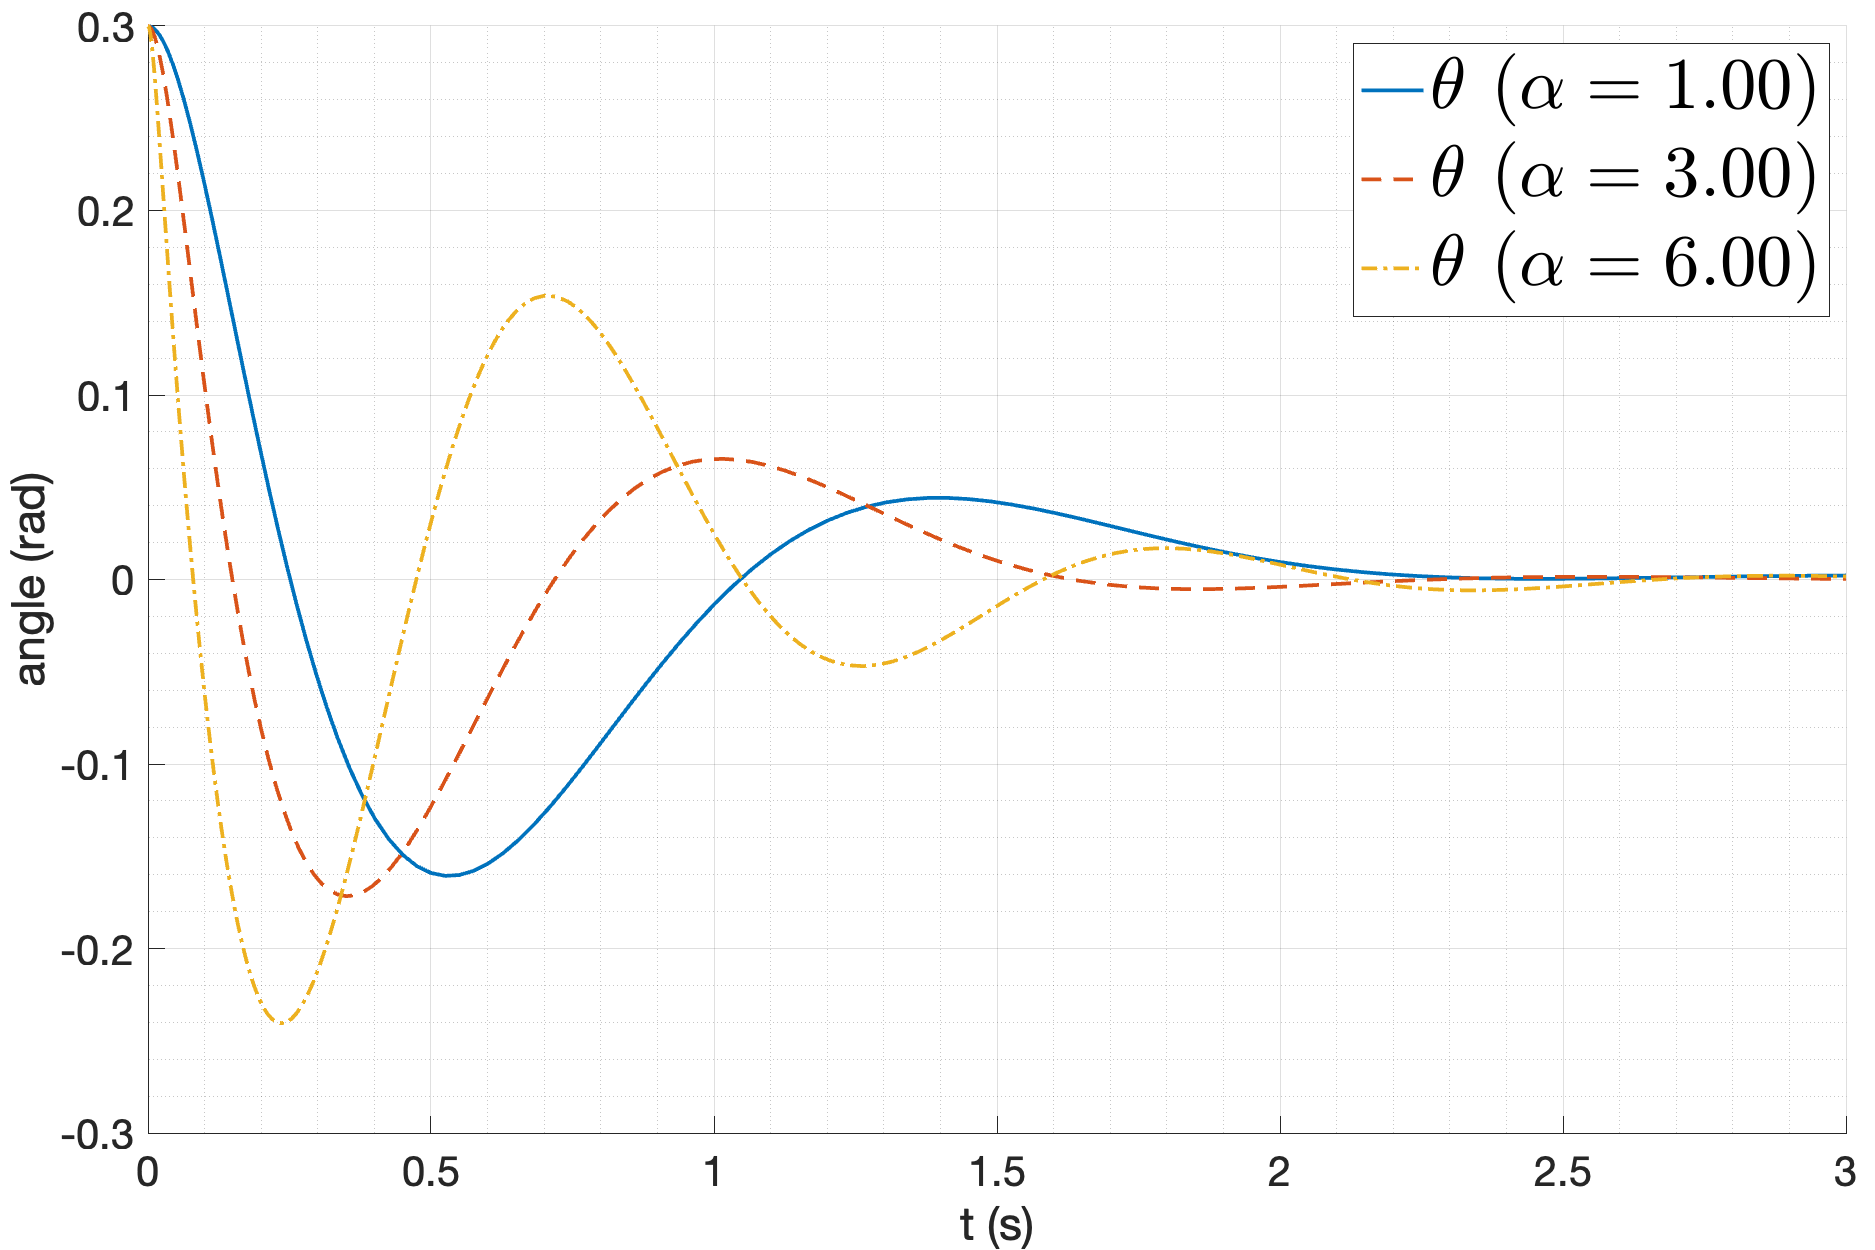
\includegraphics[width=\textwidth]{media/plots/nonmodal_controllers/ang_cmp.png}
    \caption{Сравнение переходных процессов по углу отклонения маятника}
    \label{fig:nonmodal_control_cmp_ang}
\end{figure}

\FloatBarrier
Как и ожидалось, при увеличении степени устойчивости $\alpha$ уменьшается время переходного процесса, но при этом 
увеличивается перерегулирование. При $\alpha = 1$ система стабилизируется приблизительно за $3$ секунды, а 
при $\alpha = 6$ -- за $1$ секунду. При этом, при $\alpha = 1$ максимальное отклонение от положения равновесия составляет 
$0.4$ радиан, а при $\alpha = 6$ -- $0.4$ радиан. 

Управляющее воздействие при увеличении степени устойчивости $\alpha$ также увеличивается. При $\alpha = 1$ максимальное
управляющее воздействие составляет $1500$ Н, а при $\alpha = 6$ -- $19000$. 

\subsection{Исследование регулятора с ограничением на управление} 
Рассмотрим такую же задачу нахождения регулятора, обеспечивающего заданную степень устойчивости 
системы, но теперь добавим условие минимальности управления. Неравенства в данном случае 
будут следующими:
\begin{equation}
    \begin{array}{cc}
        PA^T + AP + 2\alpha P + Y^T B^T + BY \preceq 0, ~~~ K = Y P^{-1}, ~~~ P \succ 0 \\ 
        \begin{bmatrix}
            P & x(0) \\
            x(0)^T & 1
        \end{bmatrix} \succ 0, ~~~ \begin{bmatrix}
            P & Y^T \\
            Y & \mu^2I
        \end{bmatrix} \succ 0
    \end{array}
\end{equation} 
где $\mu$ -- ограничение на управление $\mu \ge \|u(t)\|_2$.

Для синтеза регулятора зададимся начальными условиями $x_0 = \begin{bmatrix} 0 & 0 & 0.05 & 0.0 \end{bmatrix}^T$. 

Для значения $\alpha = 0.1$ получаем регулятор:
\begin{equation}
    K = \begin{bmatrix}
    3.85  & 40.27  & -2813.02  & -548.59 \\ 
    \end{bmatrix}
\end{equation}
С значением $\mu = 28.89$ и собственными числами замкнутой системы:
\begin{equation}
     \sigma(A + BK) = \begin{bmatrix}
        -5.13 \\ 
        -0.10 + 0.86j \\ 
        -0.10 - 0.86j \\ 
        -0.10 \\ 
    \end{bmatrix}
\end{equation}  
Система устойчива, степень устойчивости равна $0.1$, что в точности соответствует заданному значению $\alpha = 0.1$,
в отличие от регулятора, синтезированного без условия минимизации управляющего воздействия, где степень устойчивости 
получалась больше заданной.

Проведем моделирование данной системы при начальном угле отклонения маятника $\theta_0 = \in \begin{bmatrix} 0.05, 0.3, 0.8\end{bmatrix}$. 
Результаты моделирования приведены на рисунках \ref{fig:nonmodal_control_alpha_1_1} - \ref{fig:nonmodal_control_alpha_1_3}.
\begin{figure}[ht!]
    \centering
    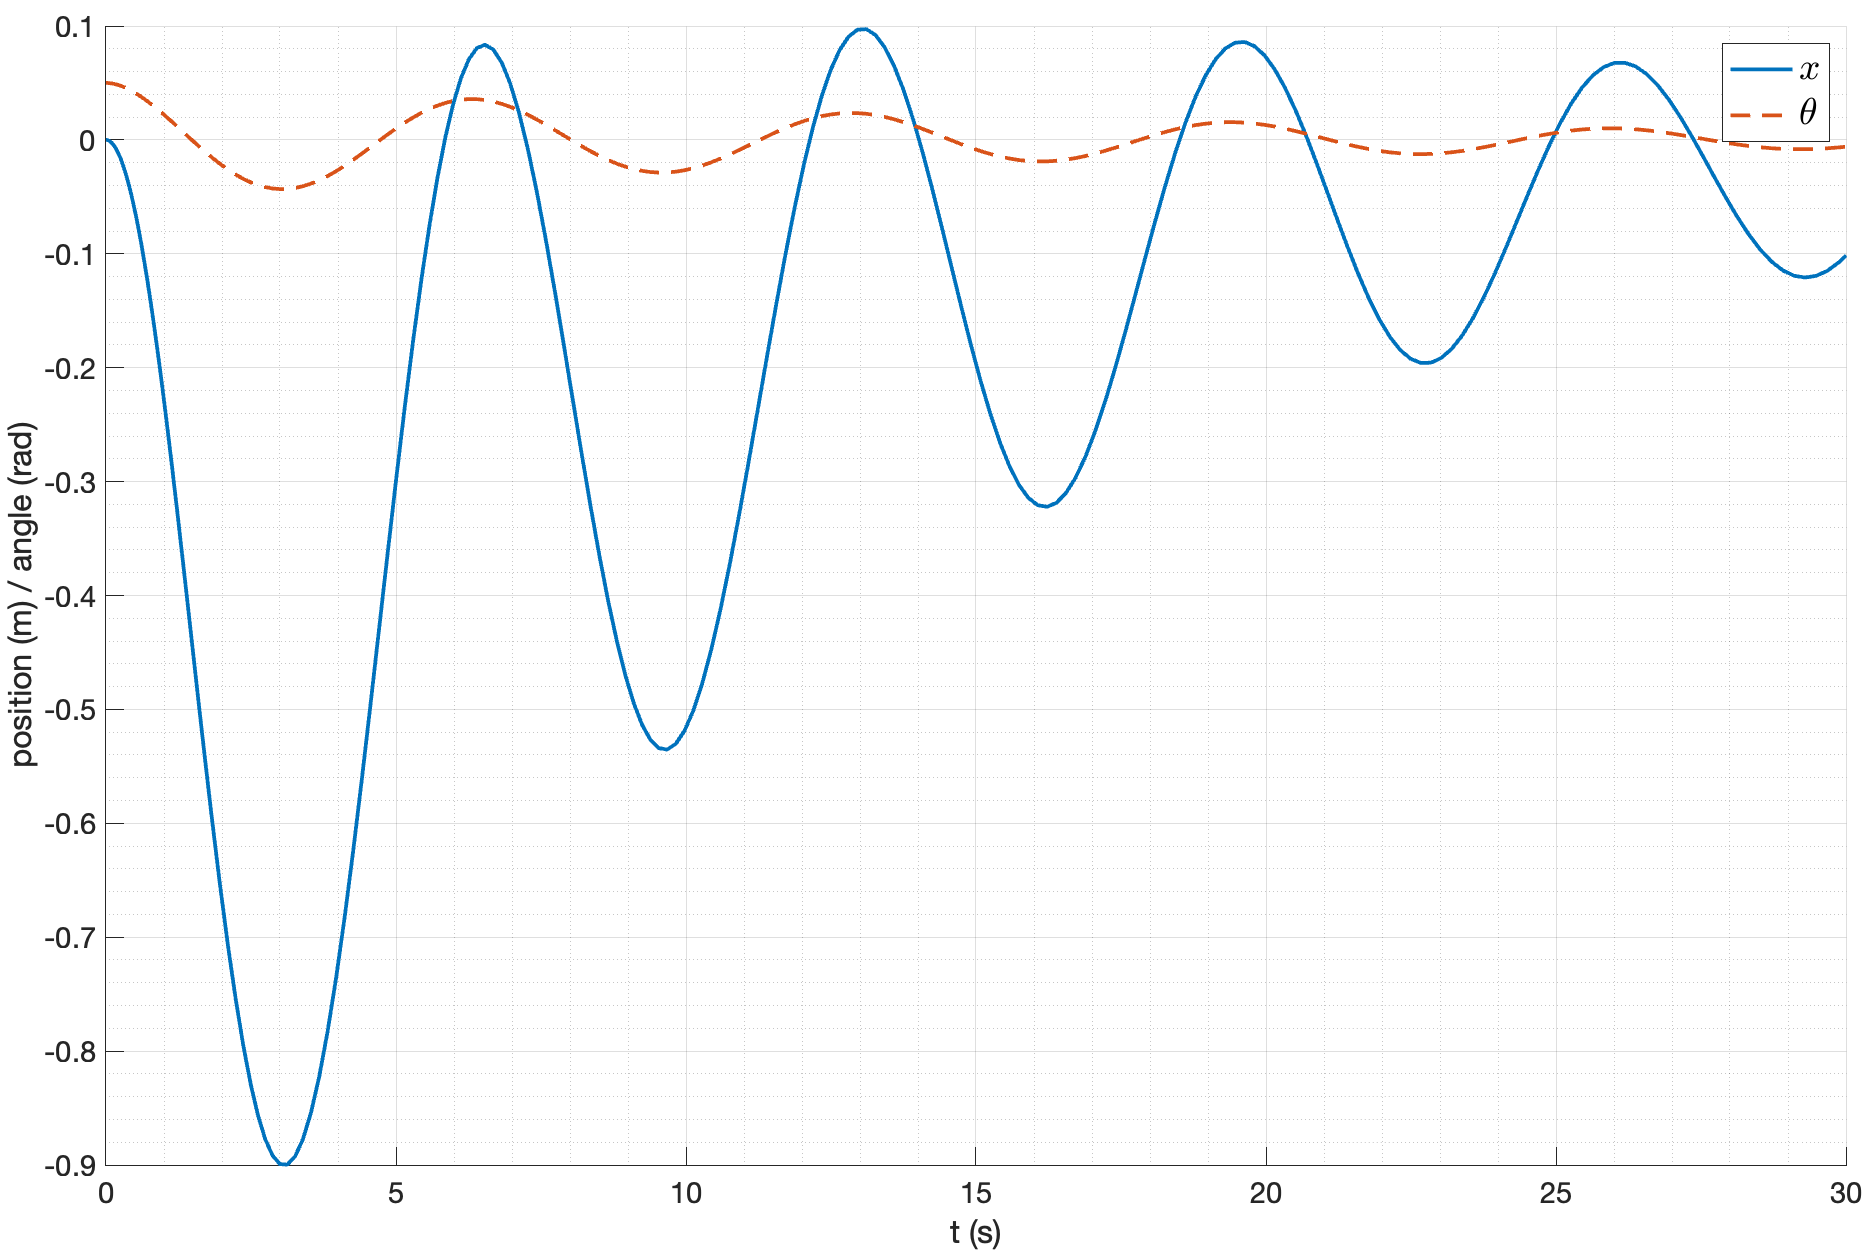
\includegraphics[width=\textwidth]{media/plots/nonmodal_controlers_min/out_1.png}
    \caption{Выход системы при $\alpha = 0.1$ и $\theta_0 = 0.05$}
    \label{fig:nonmodal_control_alpha_1_1}
\end{figure}
\begin{figure}[ht!]
    \centering
    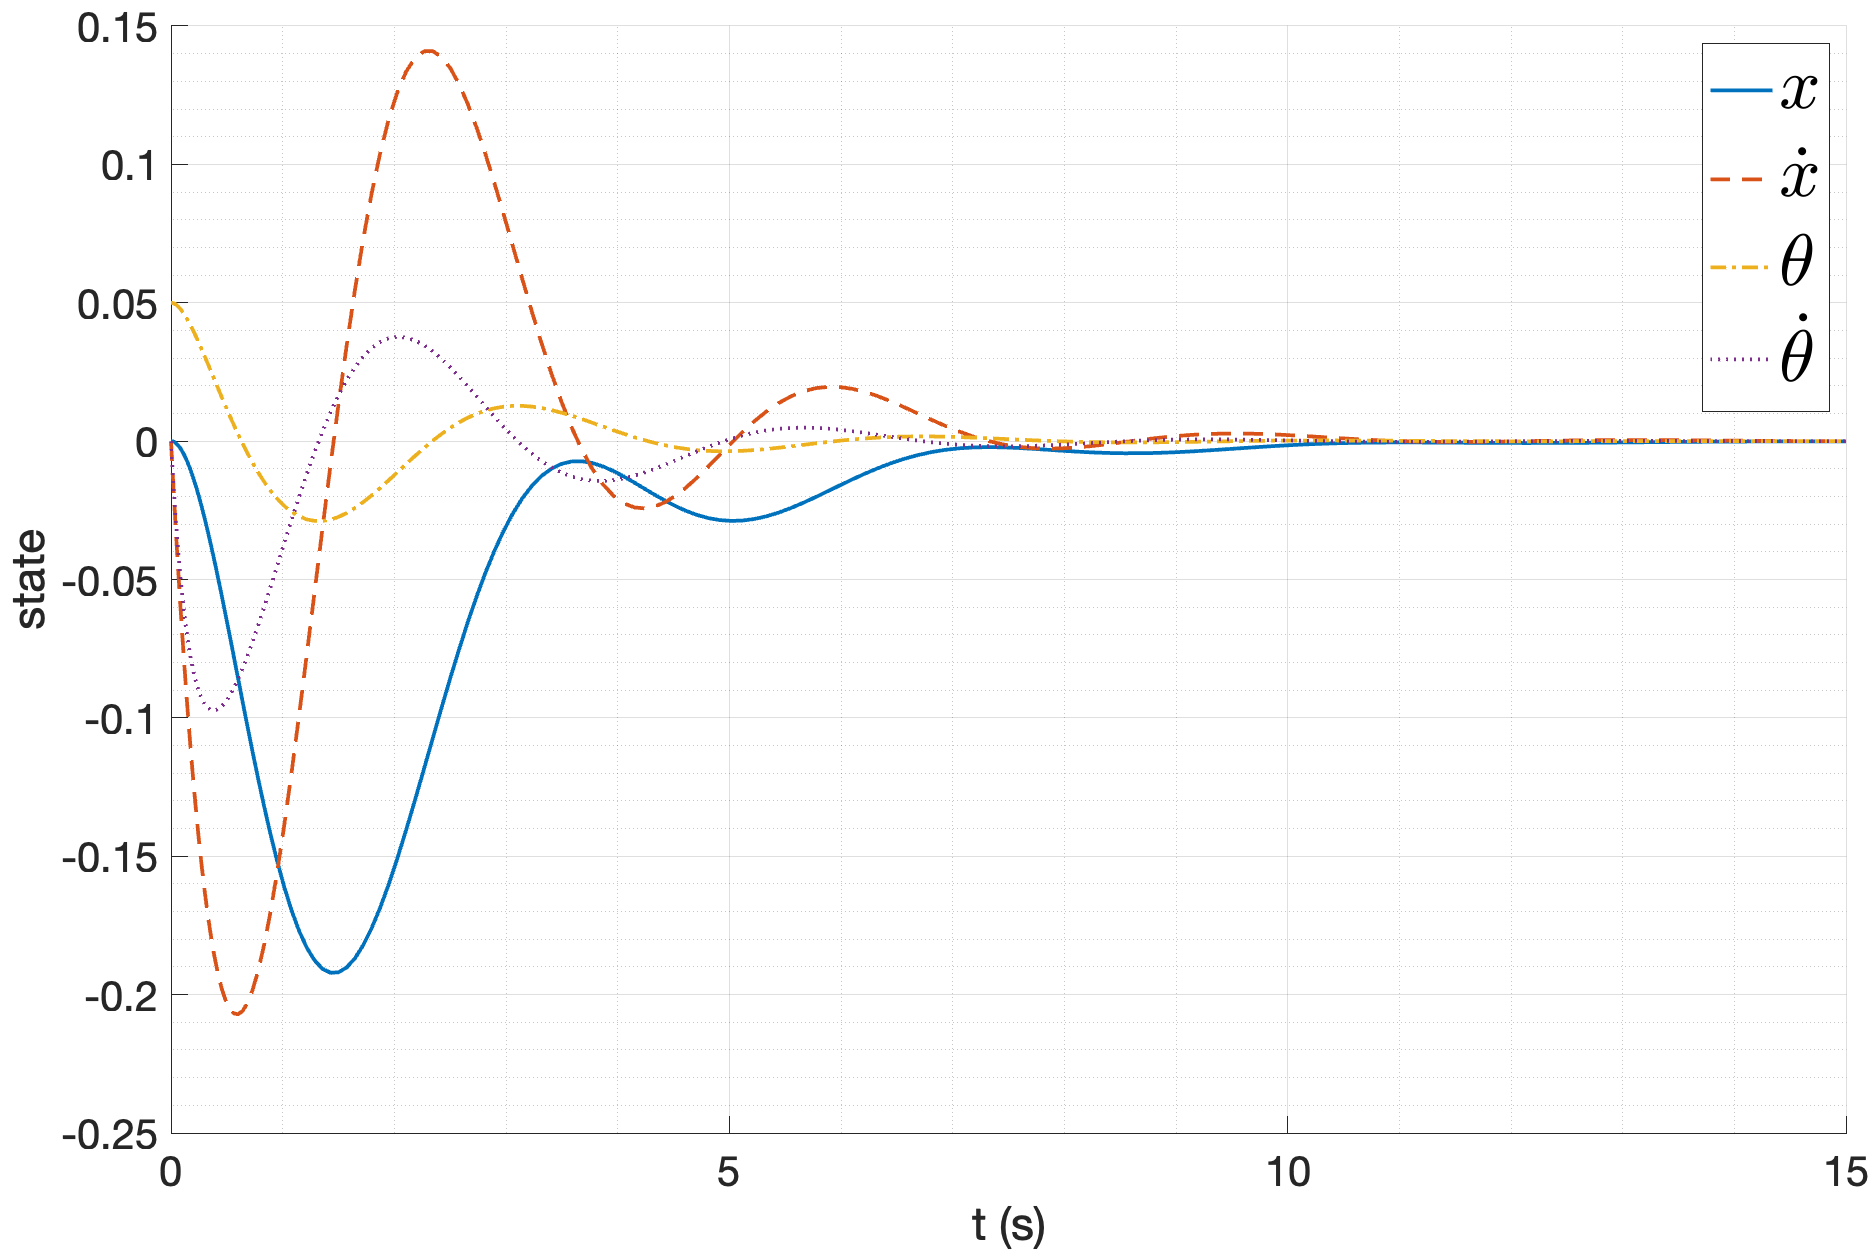
\includegraphics[width=\textwidth]{media/plots/nonmodal_controlers_min/state_1.png}
    \caption{Вектор состояния при $\alpha = 0.1$ и $\theta_0 = 0.05$}
    \label{fig:nonmodal_control_alpha_1_1_state}
\end{figure}
\begin{figure}[ht!]
    \centering
    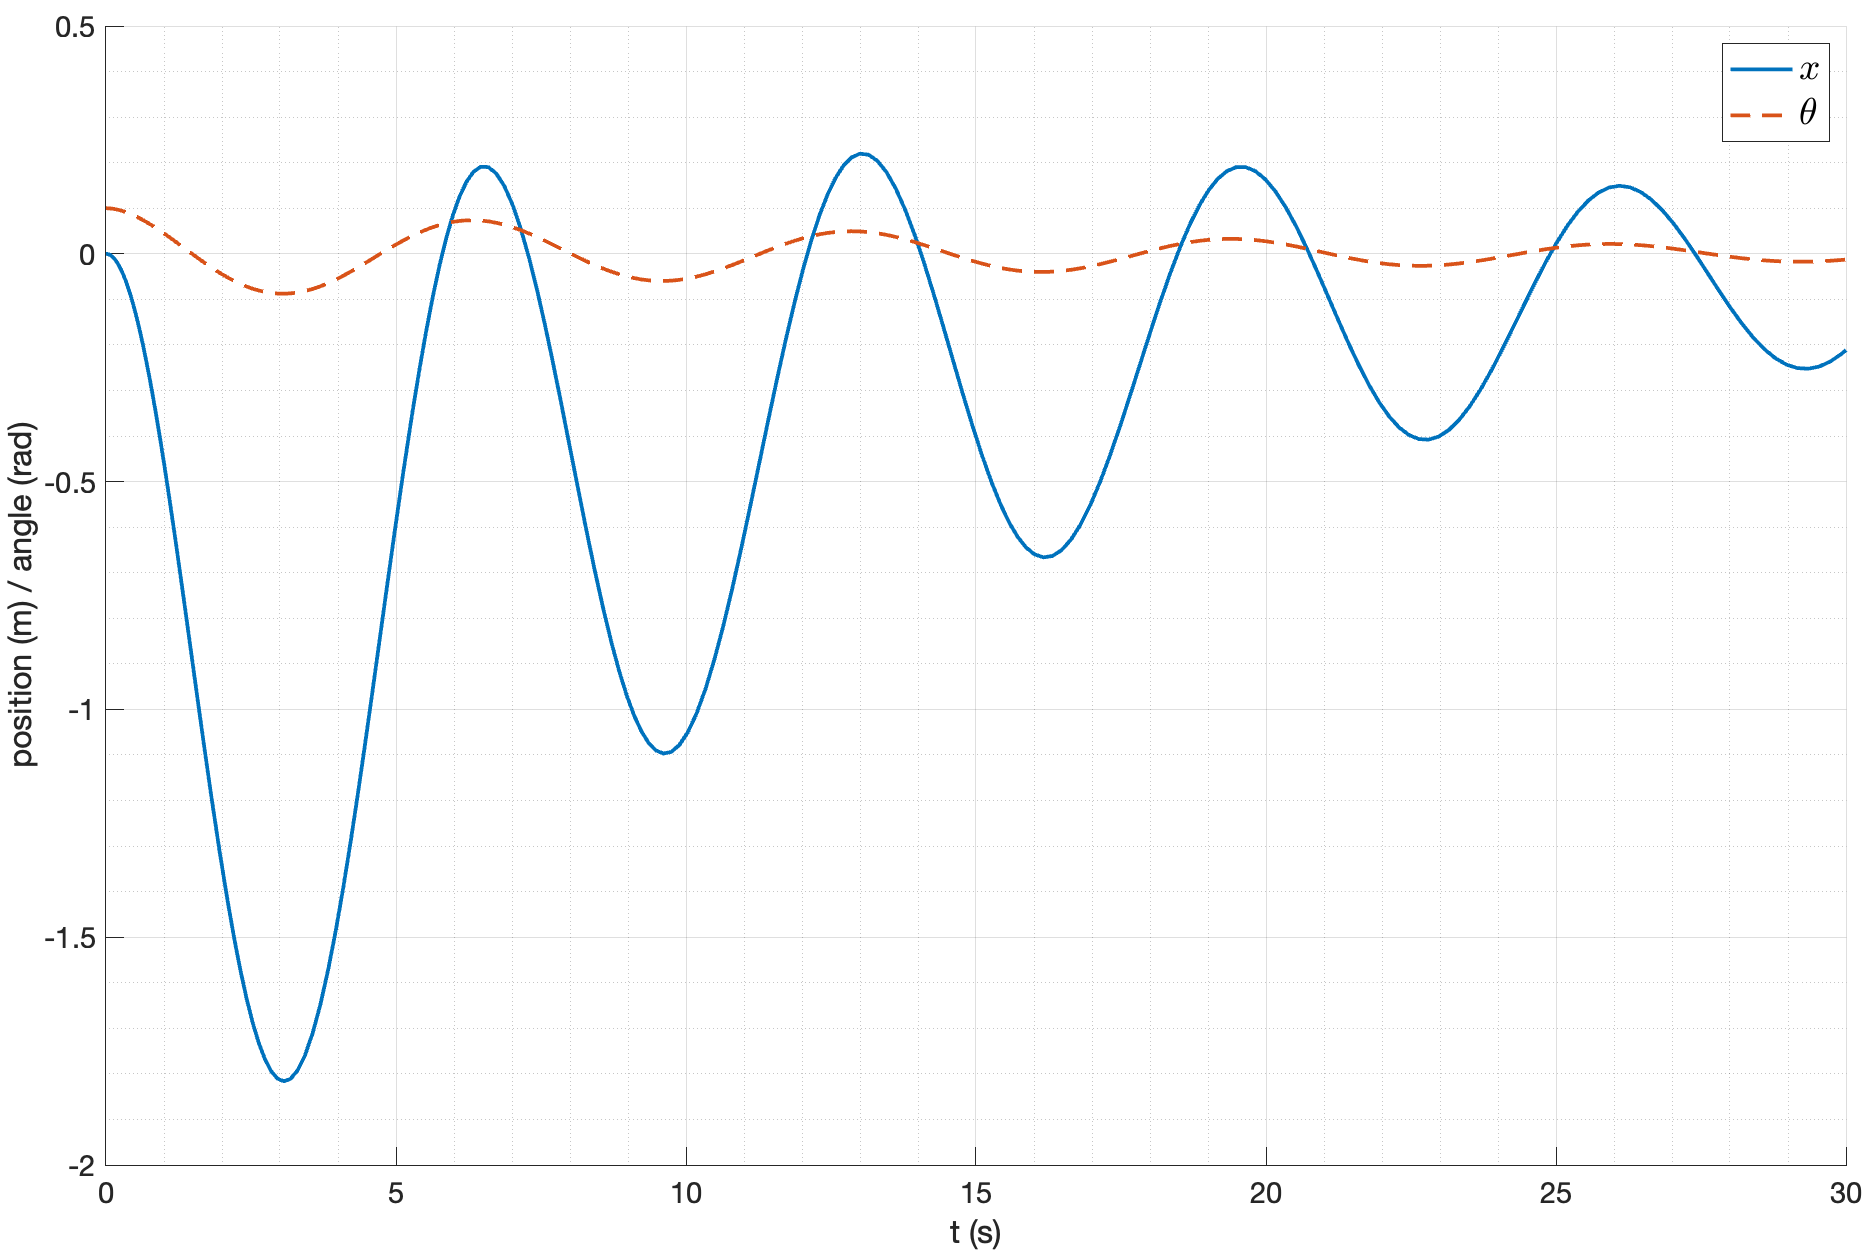
\includegraphics[width=\textwidth]{media/plots/nonmodal_controlers_min/out_2.png}
    \caption{Выход системы при $\alpha = 0.1$ и $\theta_0 = 0.3$}
    \label{fig:nonmodal_control_alpha_1_2}
\end{figure}
\begin{figure}[ht!]
    \centering
    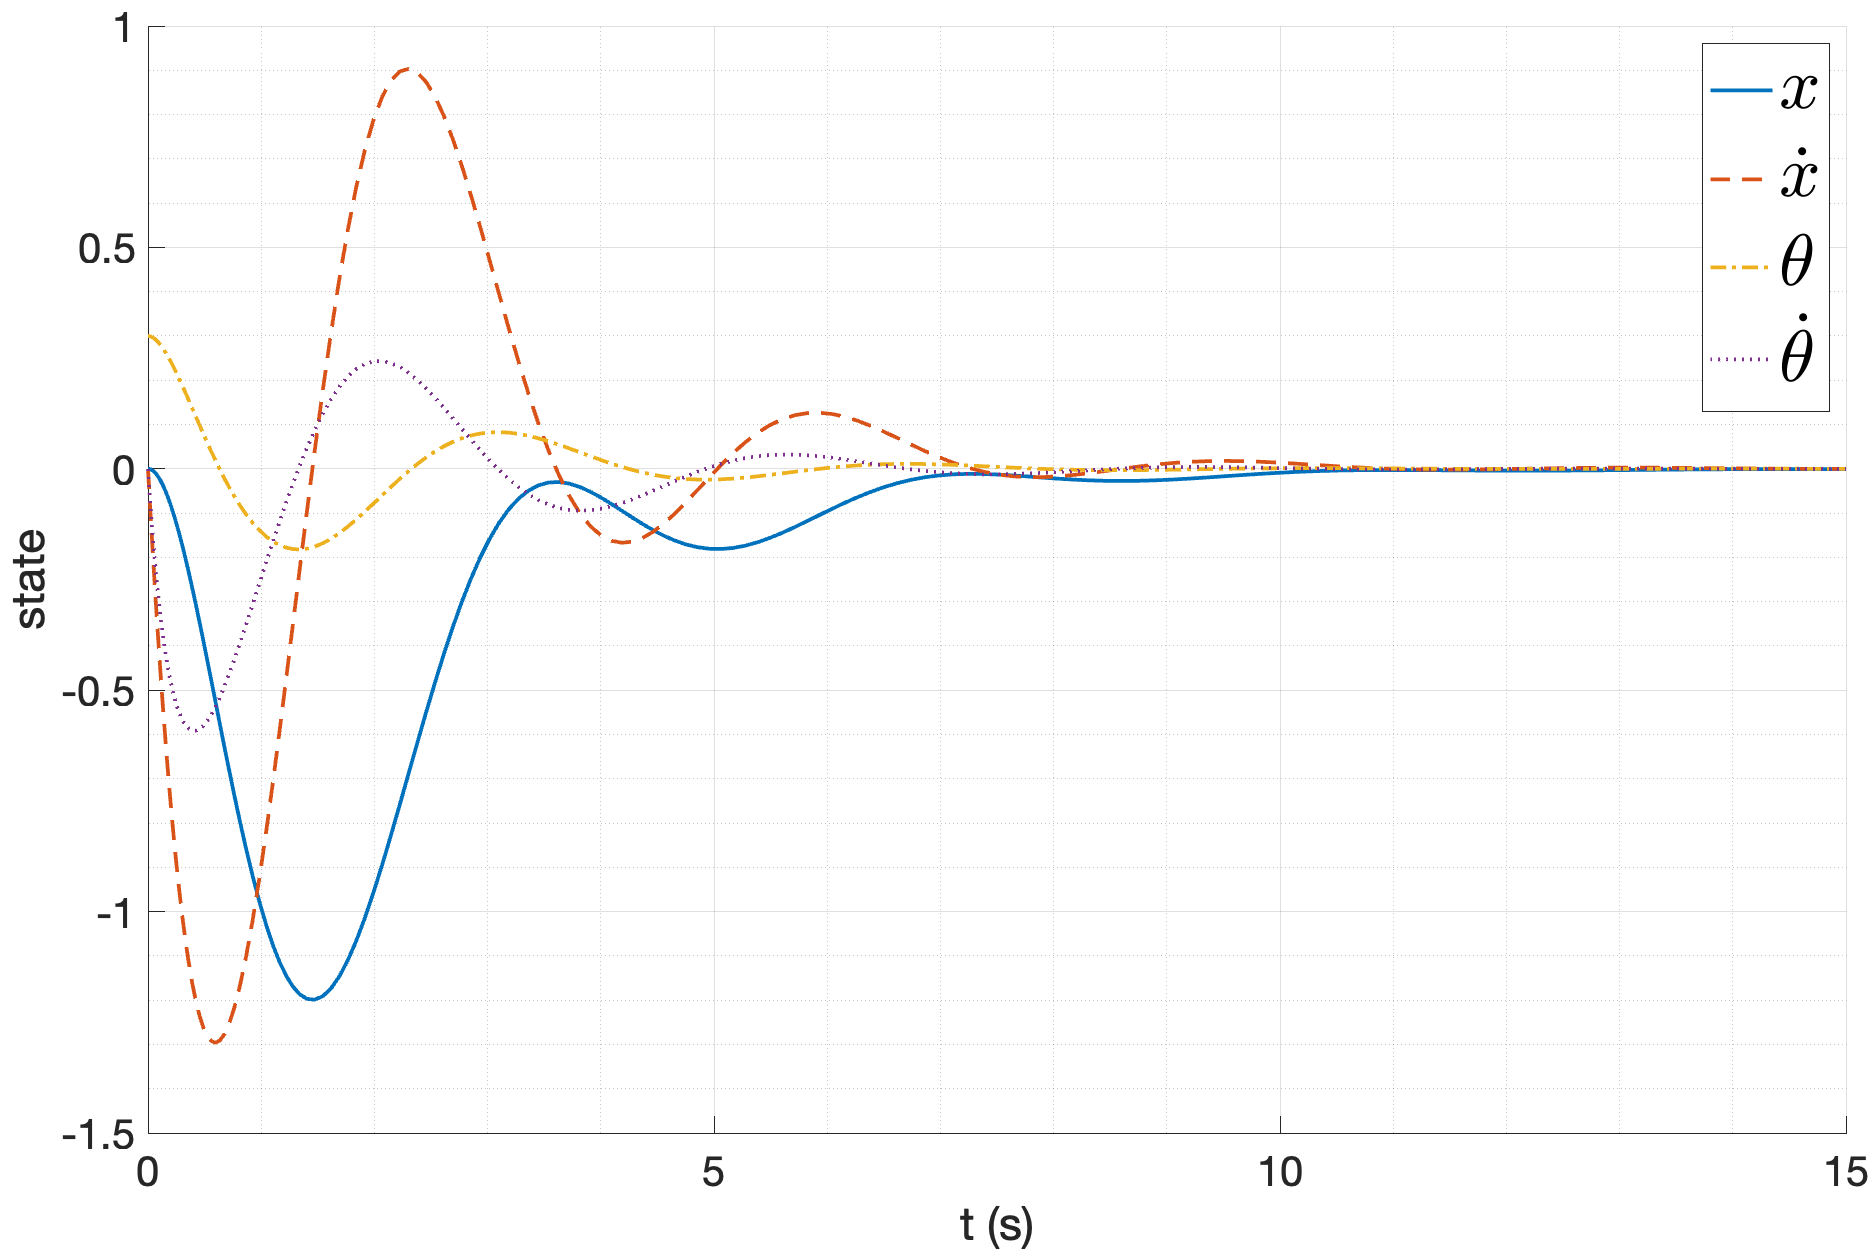
\includegraphics[width=\textwidth]{media/plots/nonmodal_controlers_min/state_2.png}
    \caption{Вектор состояния при $\alpha = 0.1$ и $\theta_0 = 0.3$}
    \label{fig:nonmodal_control_alpha_1_2_state}
\end{figure}
\begin{figure}[ht!]
    \centering
    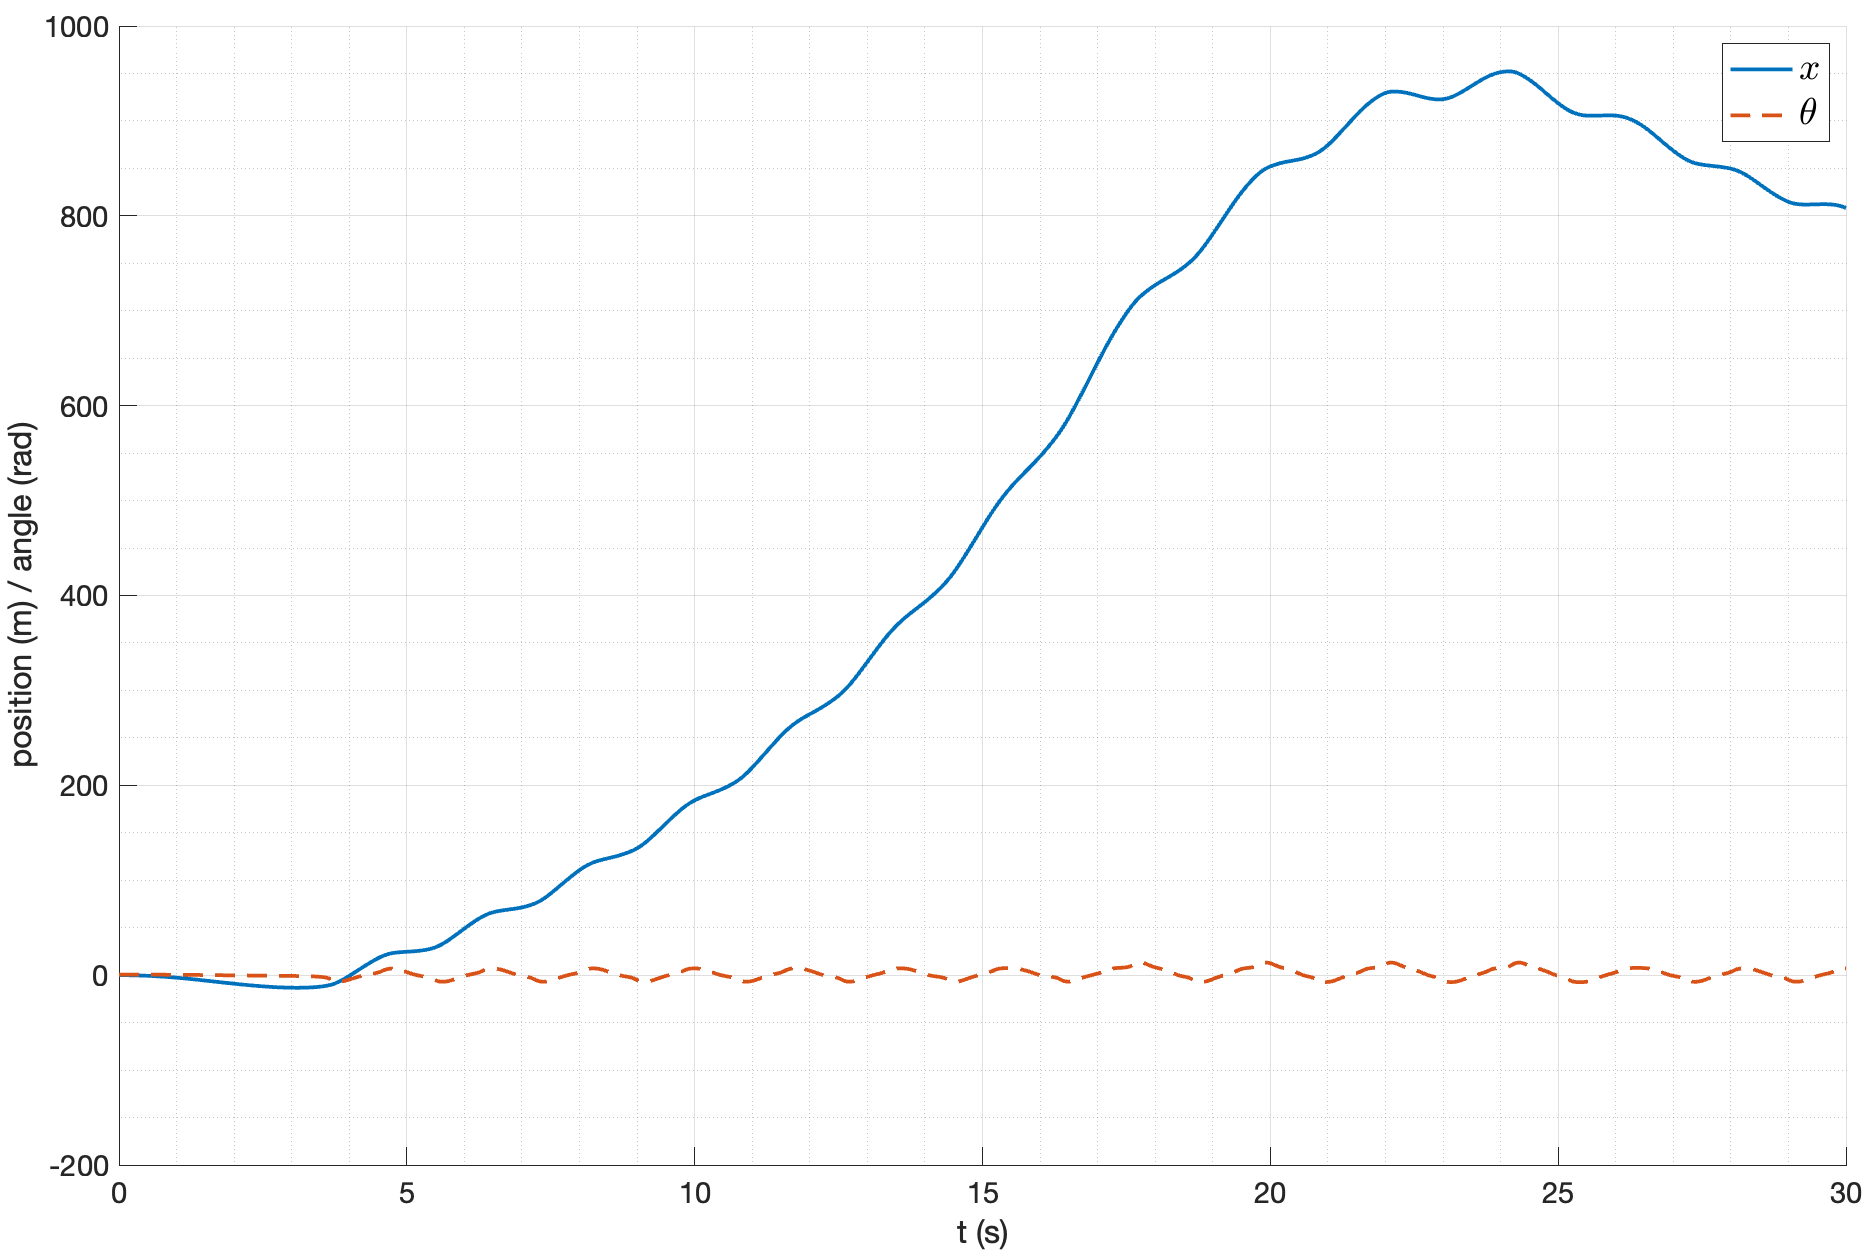
\includegraphics[width=\textwidth]{media/plots/nonmodal_controlers_min/out_3.png}
    \caption{Выход системы при $\alpha = 0.1$ и $\theta_0 = 0.8$}
    \label{fig:nonmodal_control_alpha_1_3}
\end{figure}
\begin{figure}[ht!]
    \centering
    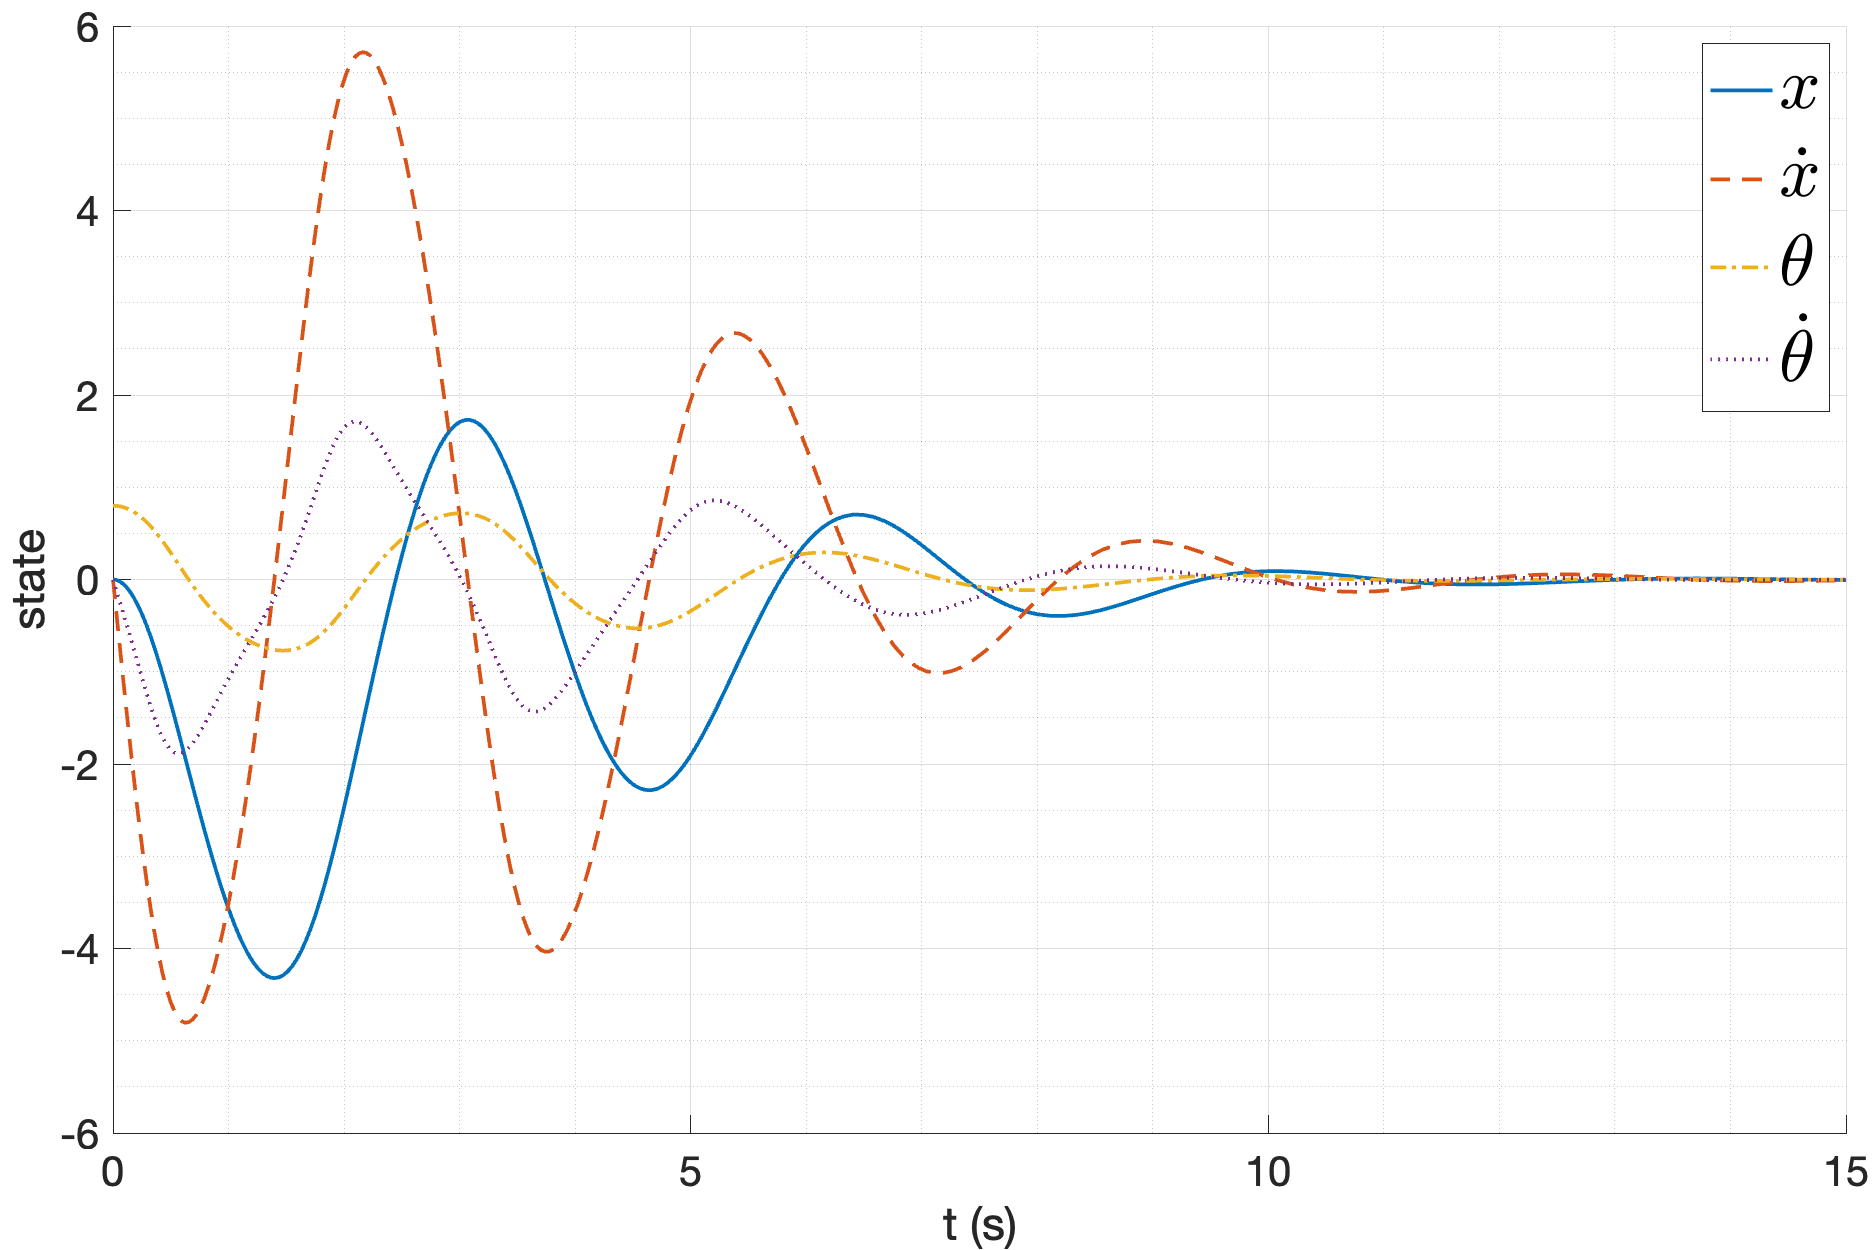
\includegraphics[width=\textwidth]{media/plots/nonmodal_controlers_min/state_3.png}
    \caption{Вектор состояния при $\alpha = 0.1$ и $\theta_0 = 0.8$}
    \label{fig:nonmodal_control_alpha_1_3_state}
\end{figure}
\FloatBarrier
Видно, что при небольших начальных условиях система стабилизируется к положению равновесия,
при этом при больших начальных условиях время стабилизации увеличивается, система начинает
больше колебаться. 
Синтез такого регулятора проводится в условиях известных начальных условий, 
и отклонение от них может привести к некорректной работе регулятора. 

\subsection{Исследование переходного процесса}
Рассмотрим поведение системы с регуляторами с различными заданными степенями устойчивости 
$\alpha \in \begin{bmatrix}0.05, 0.5, 1.0\end{bmatrix}$ и начальным углом отклонения маятника 
$\theta_0 = 0.1$. 

При $\alpha = 0.05$ получены следующие результаты: 
\begin{equation}
    K = \begin{bmatrix} 0.95  & 19.50  & -2715.72  & -613.74 \end{bmatrix}, \sigma(A + BK) = \begin{bmatrix} -4.43 \\ -0.05 + 0.56j \\ -0.05 - 0.56j \\ -0.05  \end{bmatrix}
\end{equation}
Желаемая степень устойчивости достигнута. Проведем моделирование системы. Результаты 
представлены на рисунке \ref{fig:nonmodal_control_alpha_2_1}.

\begin{figure}[ht!]
    \centering
    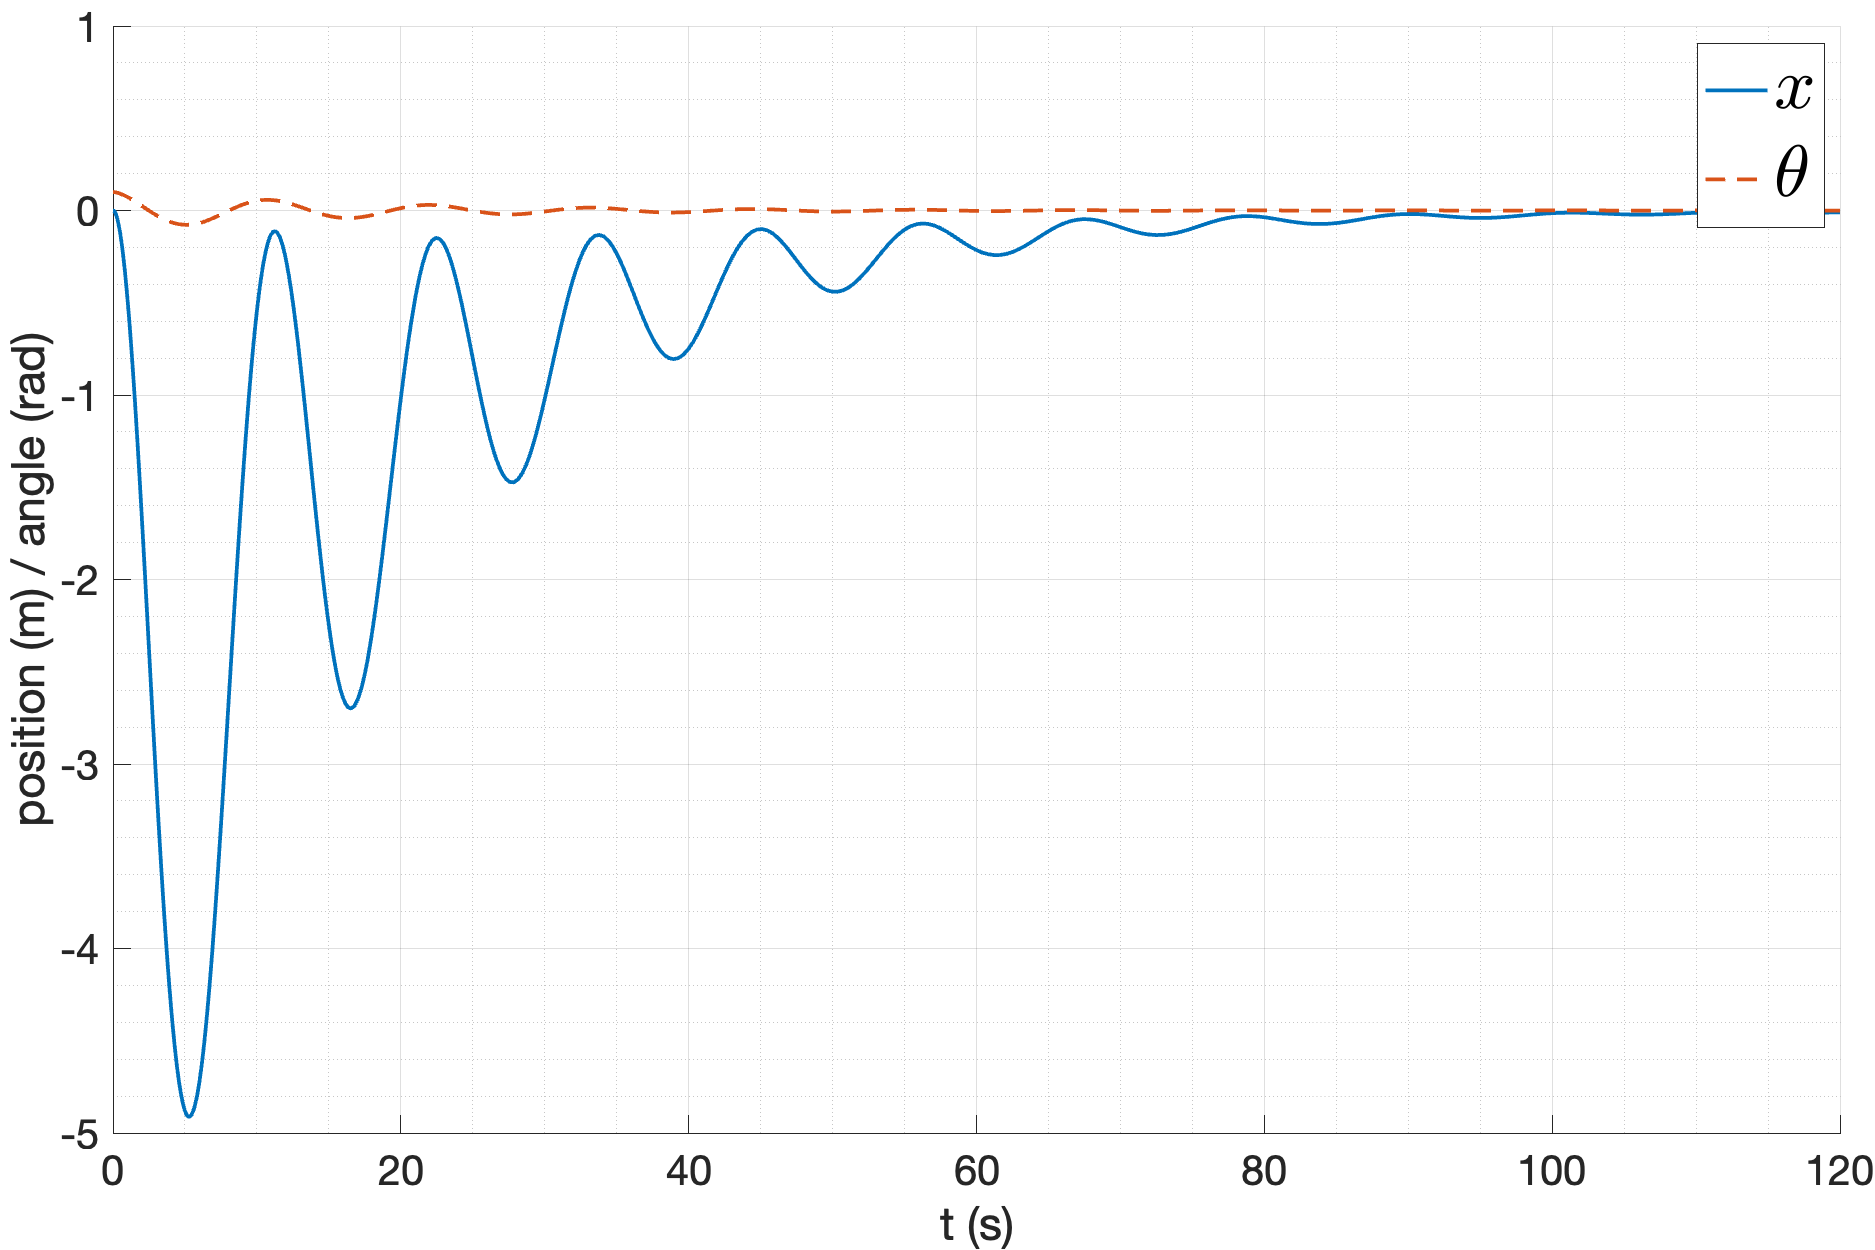
\includegraphics[width=\textwidth]{media/plots/nonmodal_controlers_min/out_4.png}
    \caption{Переходный процесс при $\alpha = 0.05$}
    \label{fig:nonmodal_control_alpha_2_1}
\end{figure}
\begin{figure}[ht!]
    \centering
    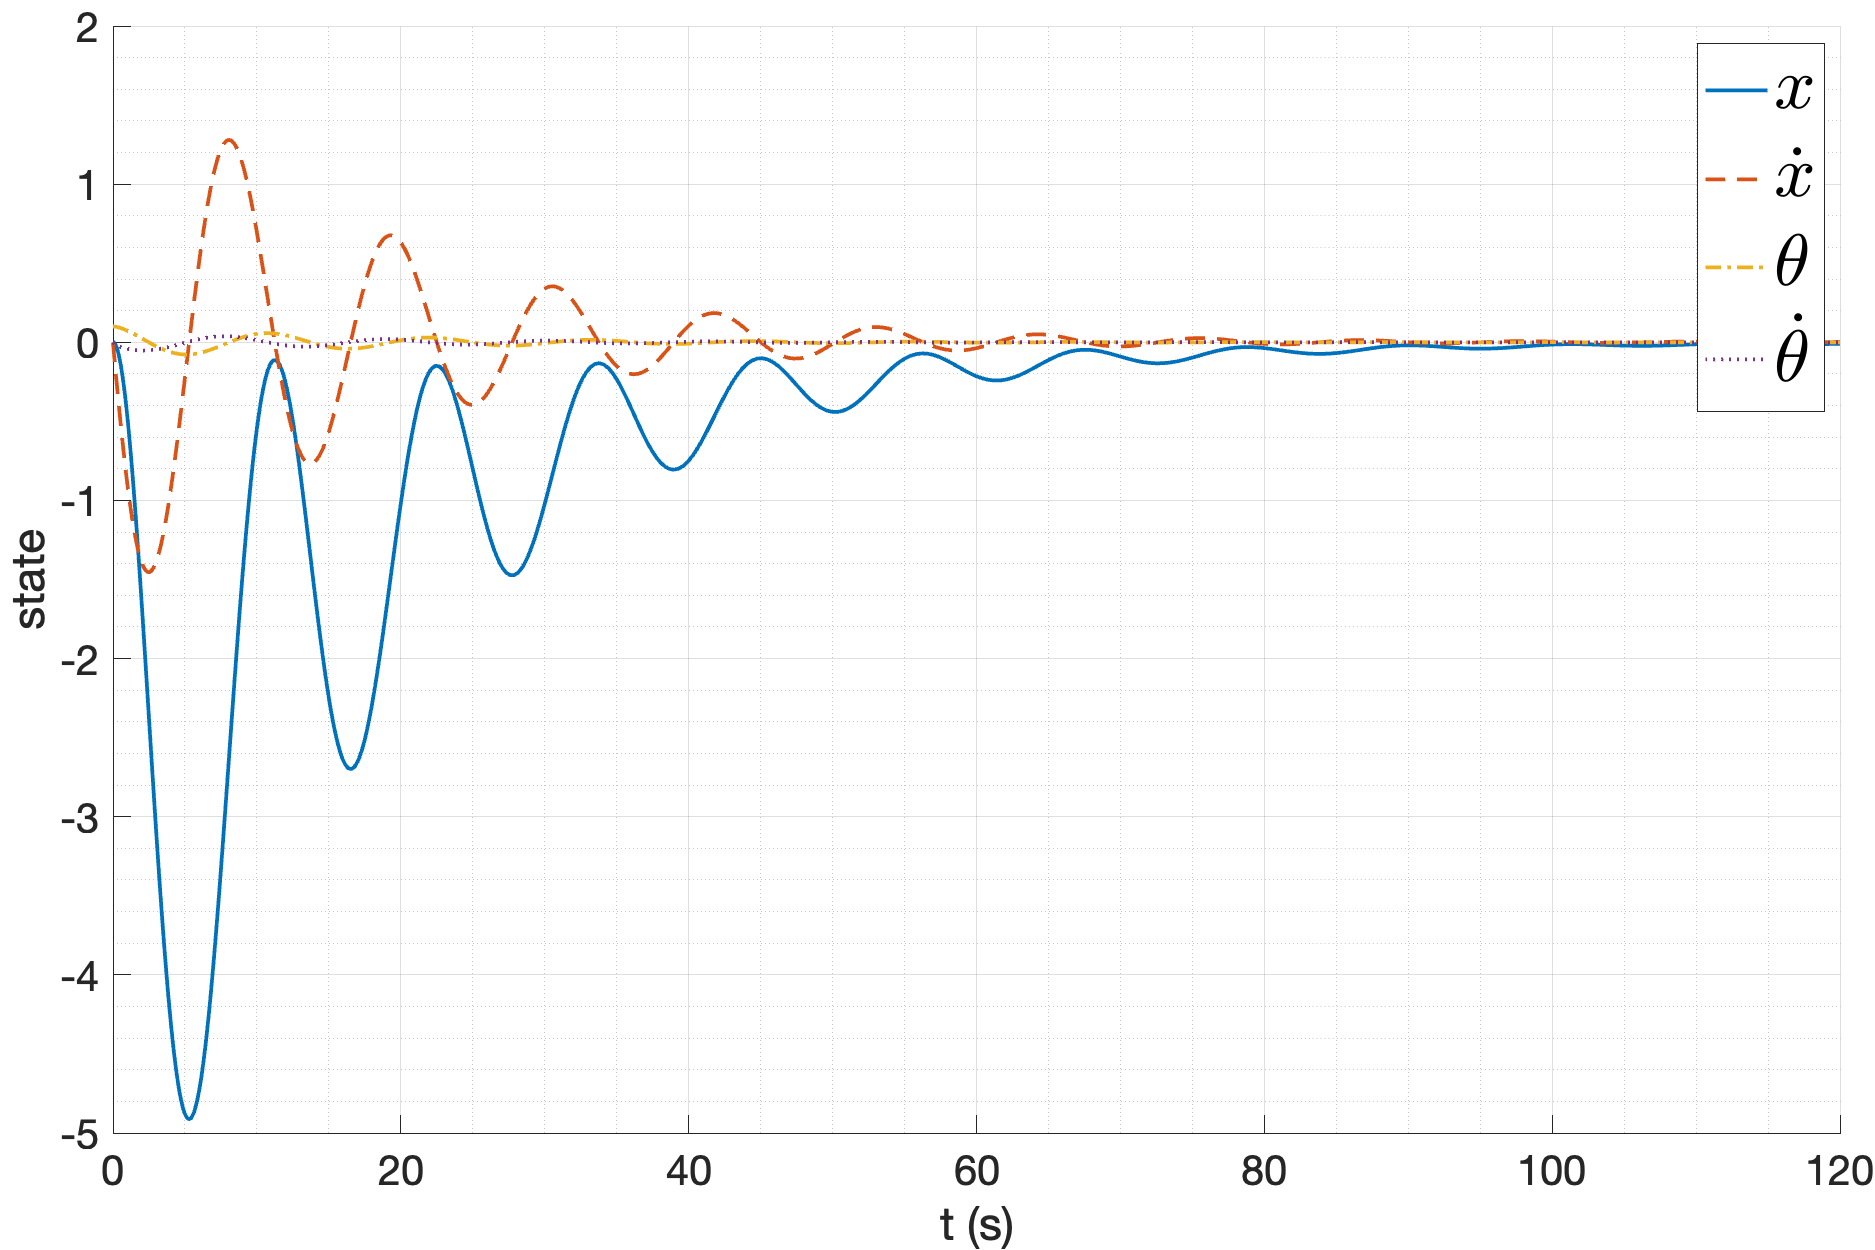
\includegraphics[width=\textwidth]{media/plots/nonmodal_controlers_min/state_4.png}
    \caption{Вектор состояния при $\alpha = 0.05$}
    \label{fig:nonmodal_control_alpha_2_1_state}
\end{figure}

\FloatBarrier
При $\alpha = 0.5$ получены следующие результаты: 
\begin{equation}
    K = \begin{bmatrix} 111.01  & 276.86  & -4075.74  & -923.80  \\ \end{bmatrix}, \sigma(A + BK) = \begin{bmatrix} -4.43 \\ -0.50 + 1.87j \\ -0.50 - 1.87j \\ -0.50 \\ \end{bmatrix}
\end{equation}
Желаемая степень устойчивости достигнута. Проведем моделирование системы. Результаты 
представлены на рисунках \ref{fig:nonmodal_control_alpha_2_1} - \ref{fig:nonmodal_control_alpha_2_3}

\begin{figure}[ht!]
    \centering
    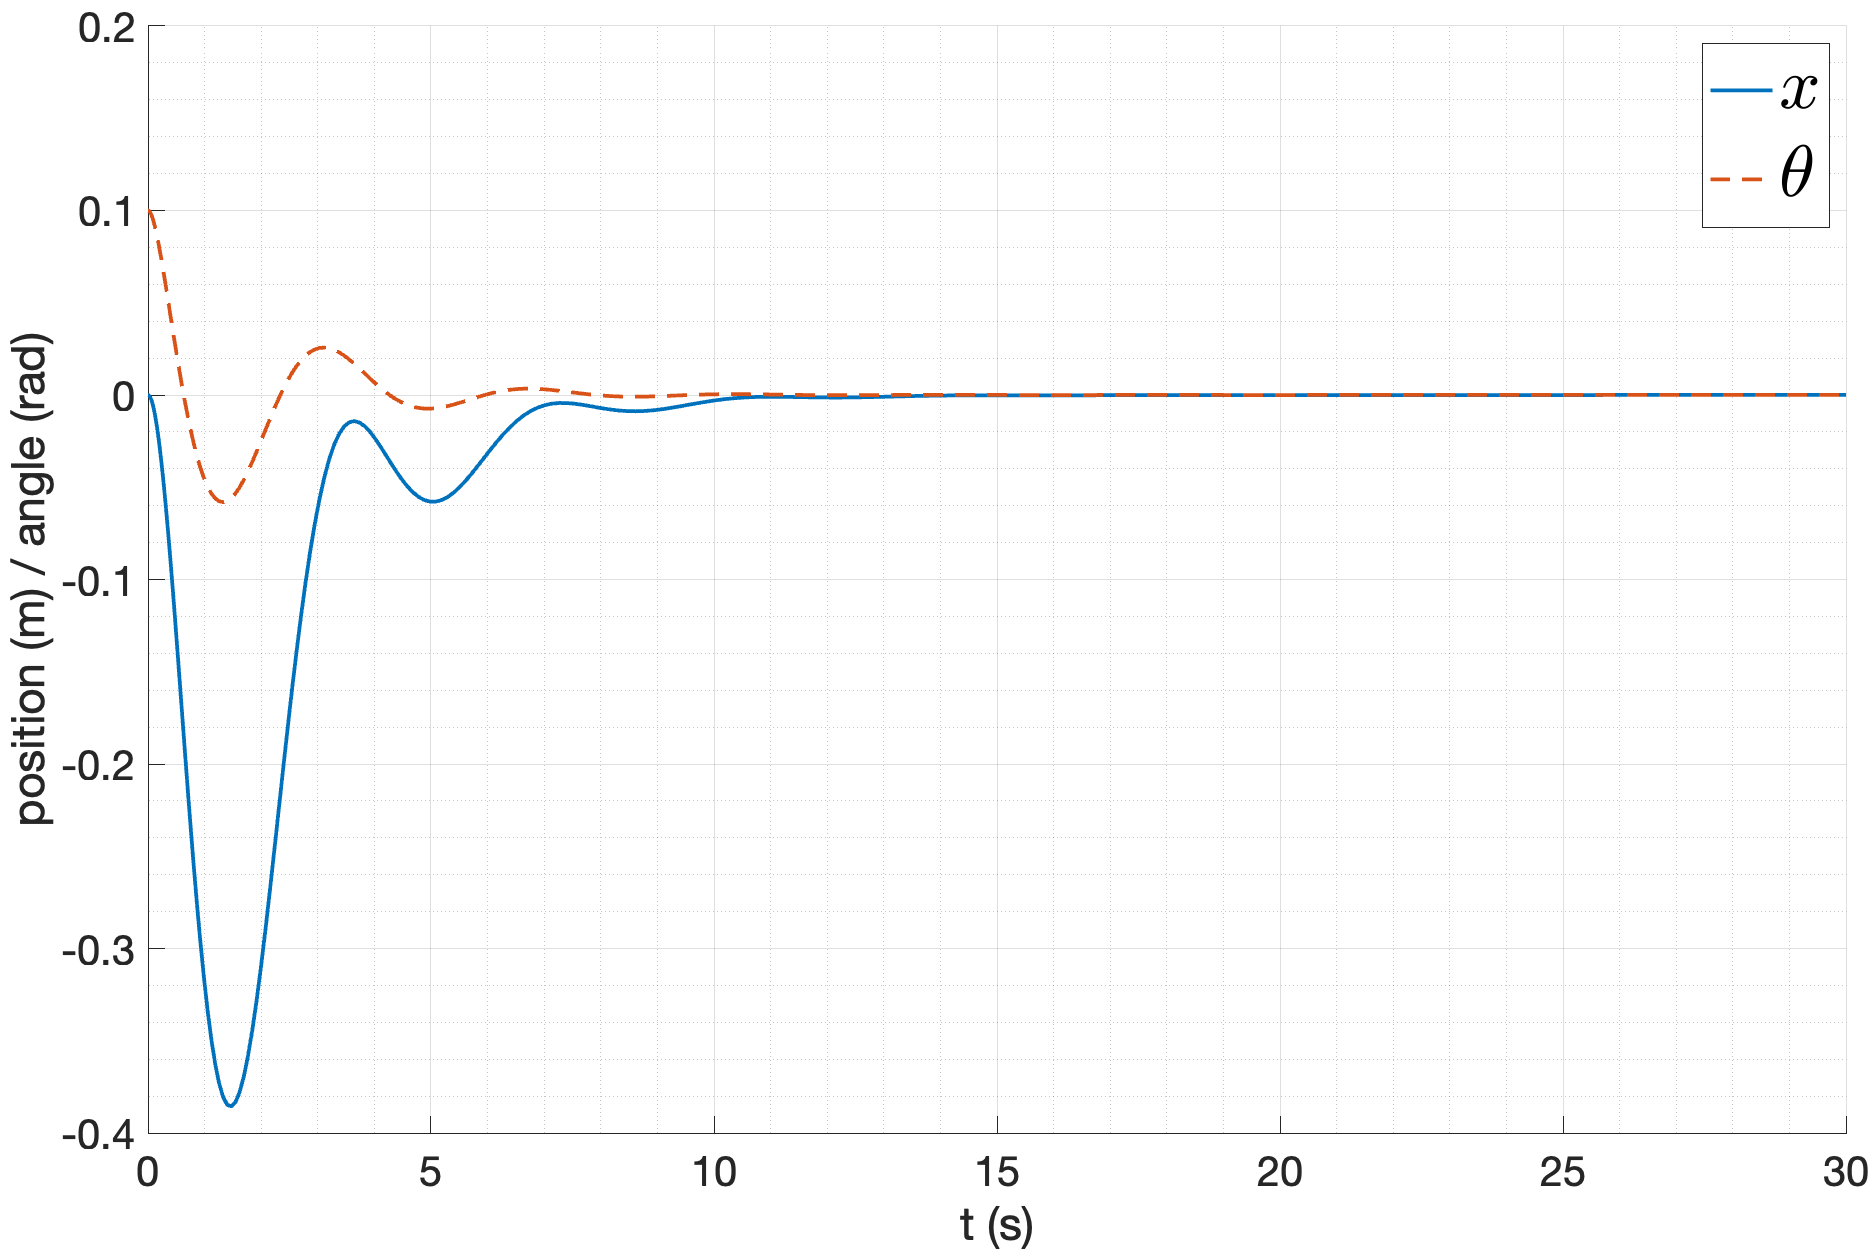
\includegraphics[width=\textwidth]{media/plots/nonmodal_controlers_min/out_5.png}
    \caption{Переходный процесс при $\alpha = 0.5$}
    \label{fig:nonmodal_control_alpha_2_2}
\end{figure} 
\begin{figure}[ht!]
    \centering
    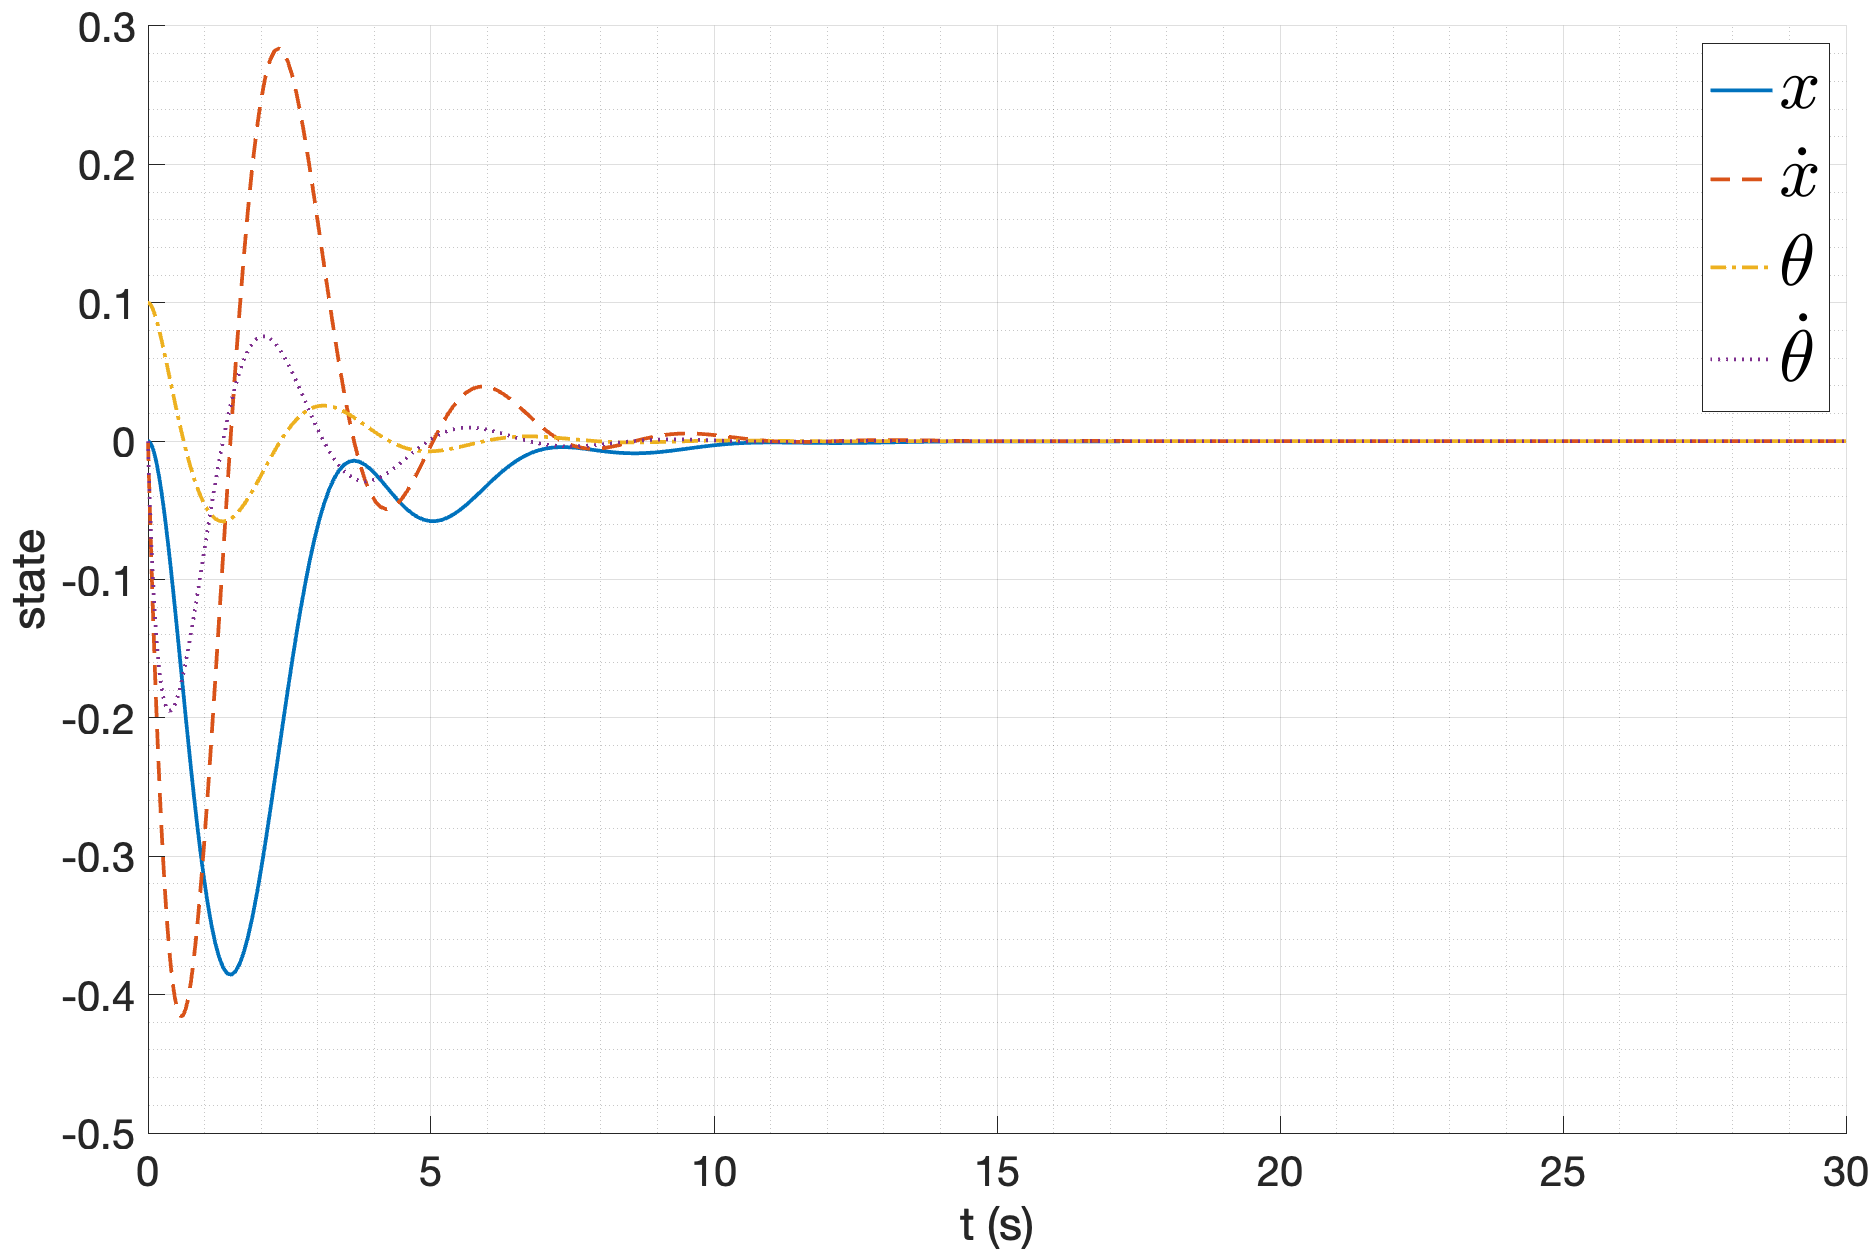
\includegraphics[width=\textwidth]{media/plots/nonmodal_controlers_min/state_5.png}
    \caption{Вектор состояния при $\alpha = 0.5$}
    \label{fig:nonmodal_control_alpha_2_2_state}
\end{figure}

\FloatBarrier
При $\alpha = 1.0$ получены следующие результаты: 
\begin{equation}
    K = \begin{bmatrix} -14.94  & -22.76  & 1.78  & 0.64  \end{bmatrix}, \sigma(A + BK) = \begin{bmatrix} -4.43 \\ -0.04 + 0.23j \\ -0.04 - 0.23j \\ 4.43 \\ \end{bmatrix}
\end{equation}
Решение данной системы не было найдено, собственные числа системы не соответствуют заданной степени устойчивости.
Кроме того, с полученным регулятором система не является устойчивой, что связано с наличием 
собственного числа с положительной действительной частью.

\begin{figure}[ht!]
    \centering
    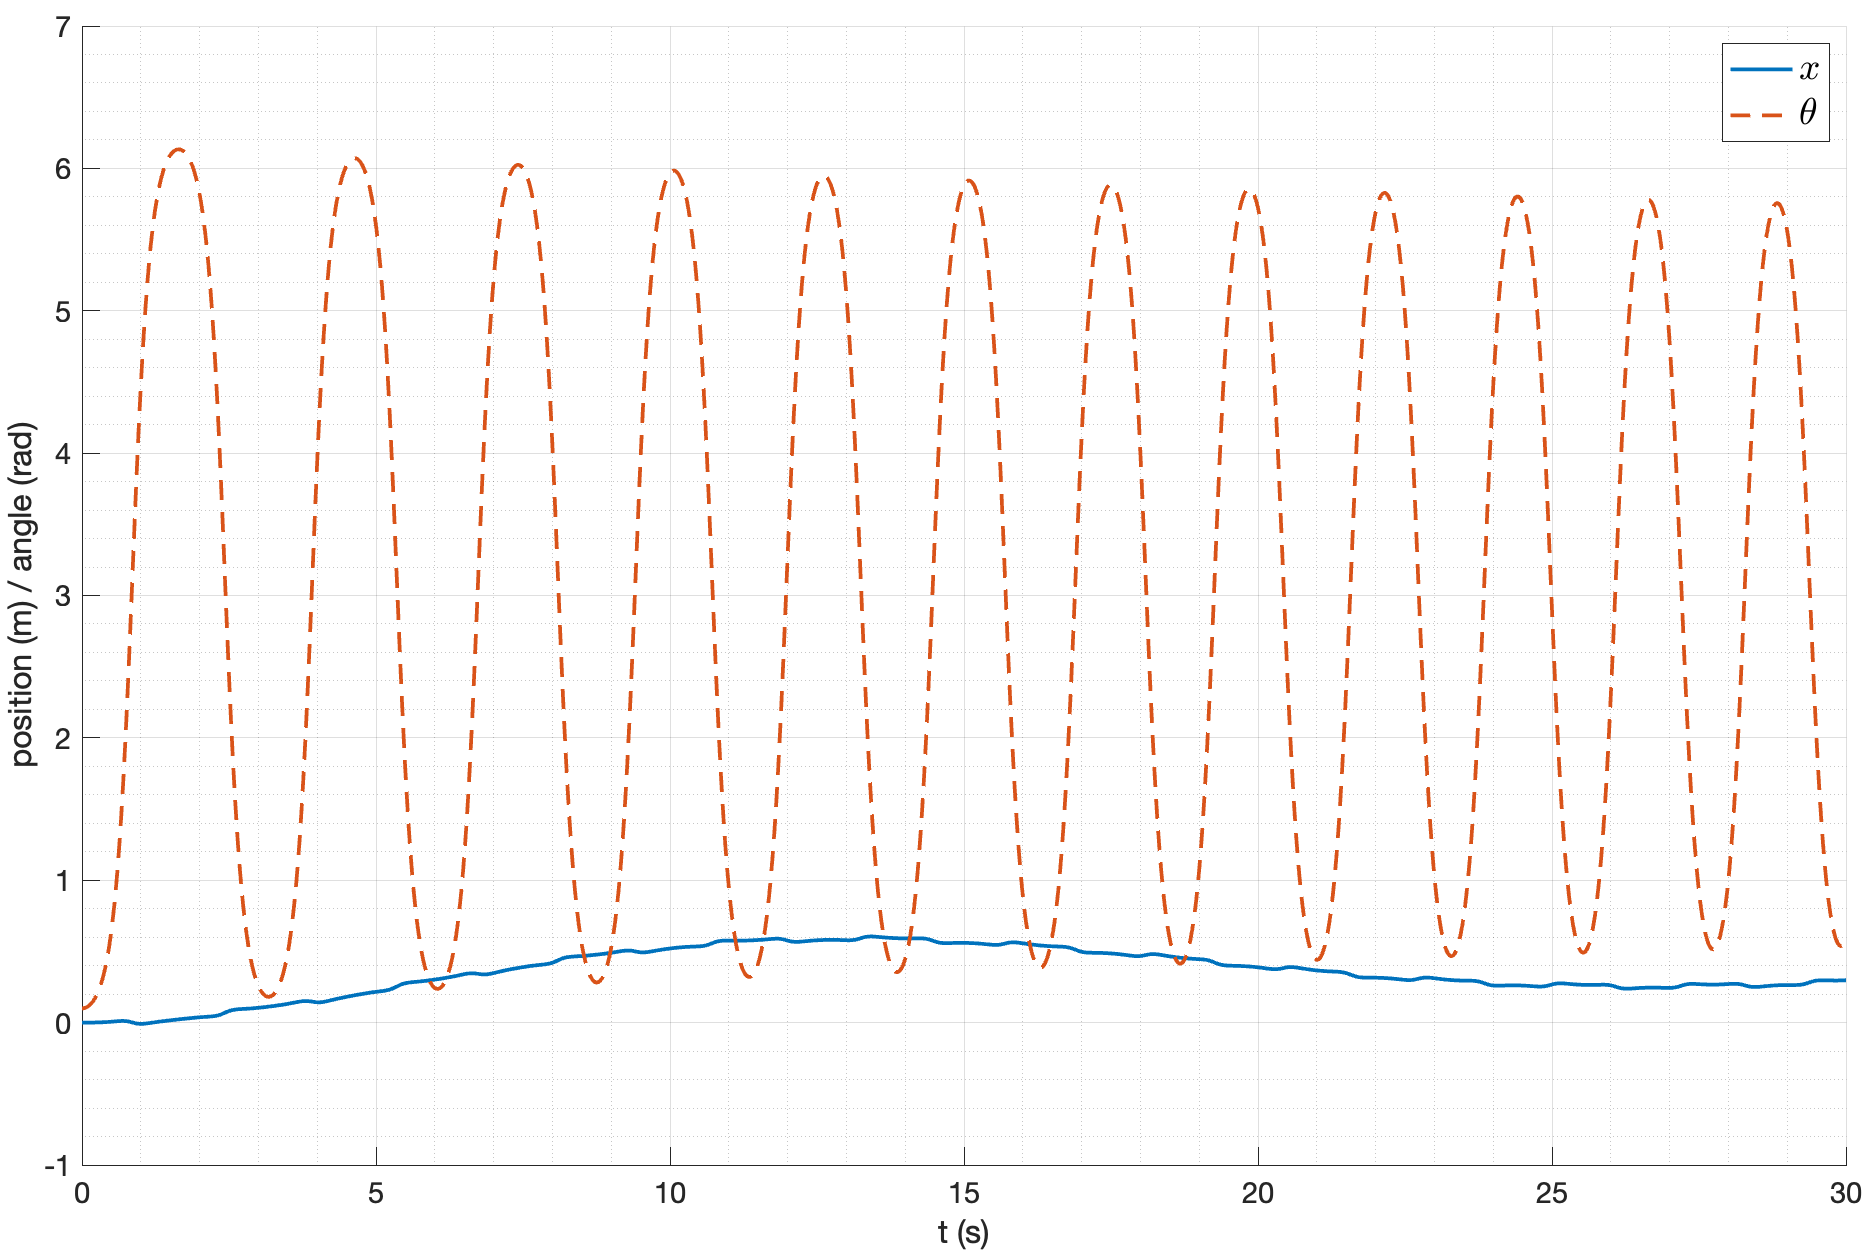
\includegraphics[width=\textwidth]{media/plots/nonmodal_controlers_min/out_6.png}
    \caption{Переходный процесс при $\alpha = 1.0$}
    \label{fig:nonmodal_control_alpha_2_3}
\end{figure} 
\begin{figure}[ht!]
    \centering
    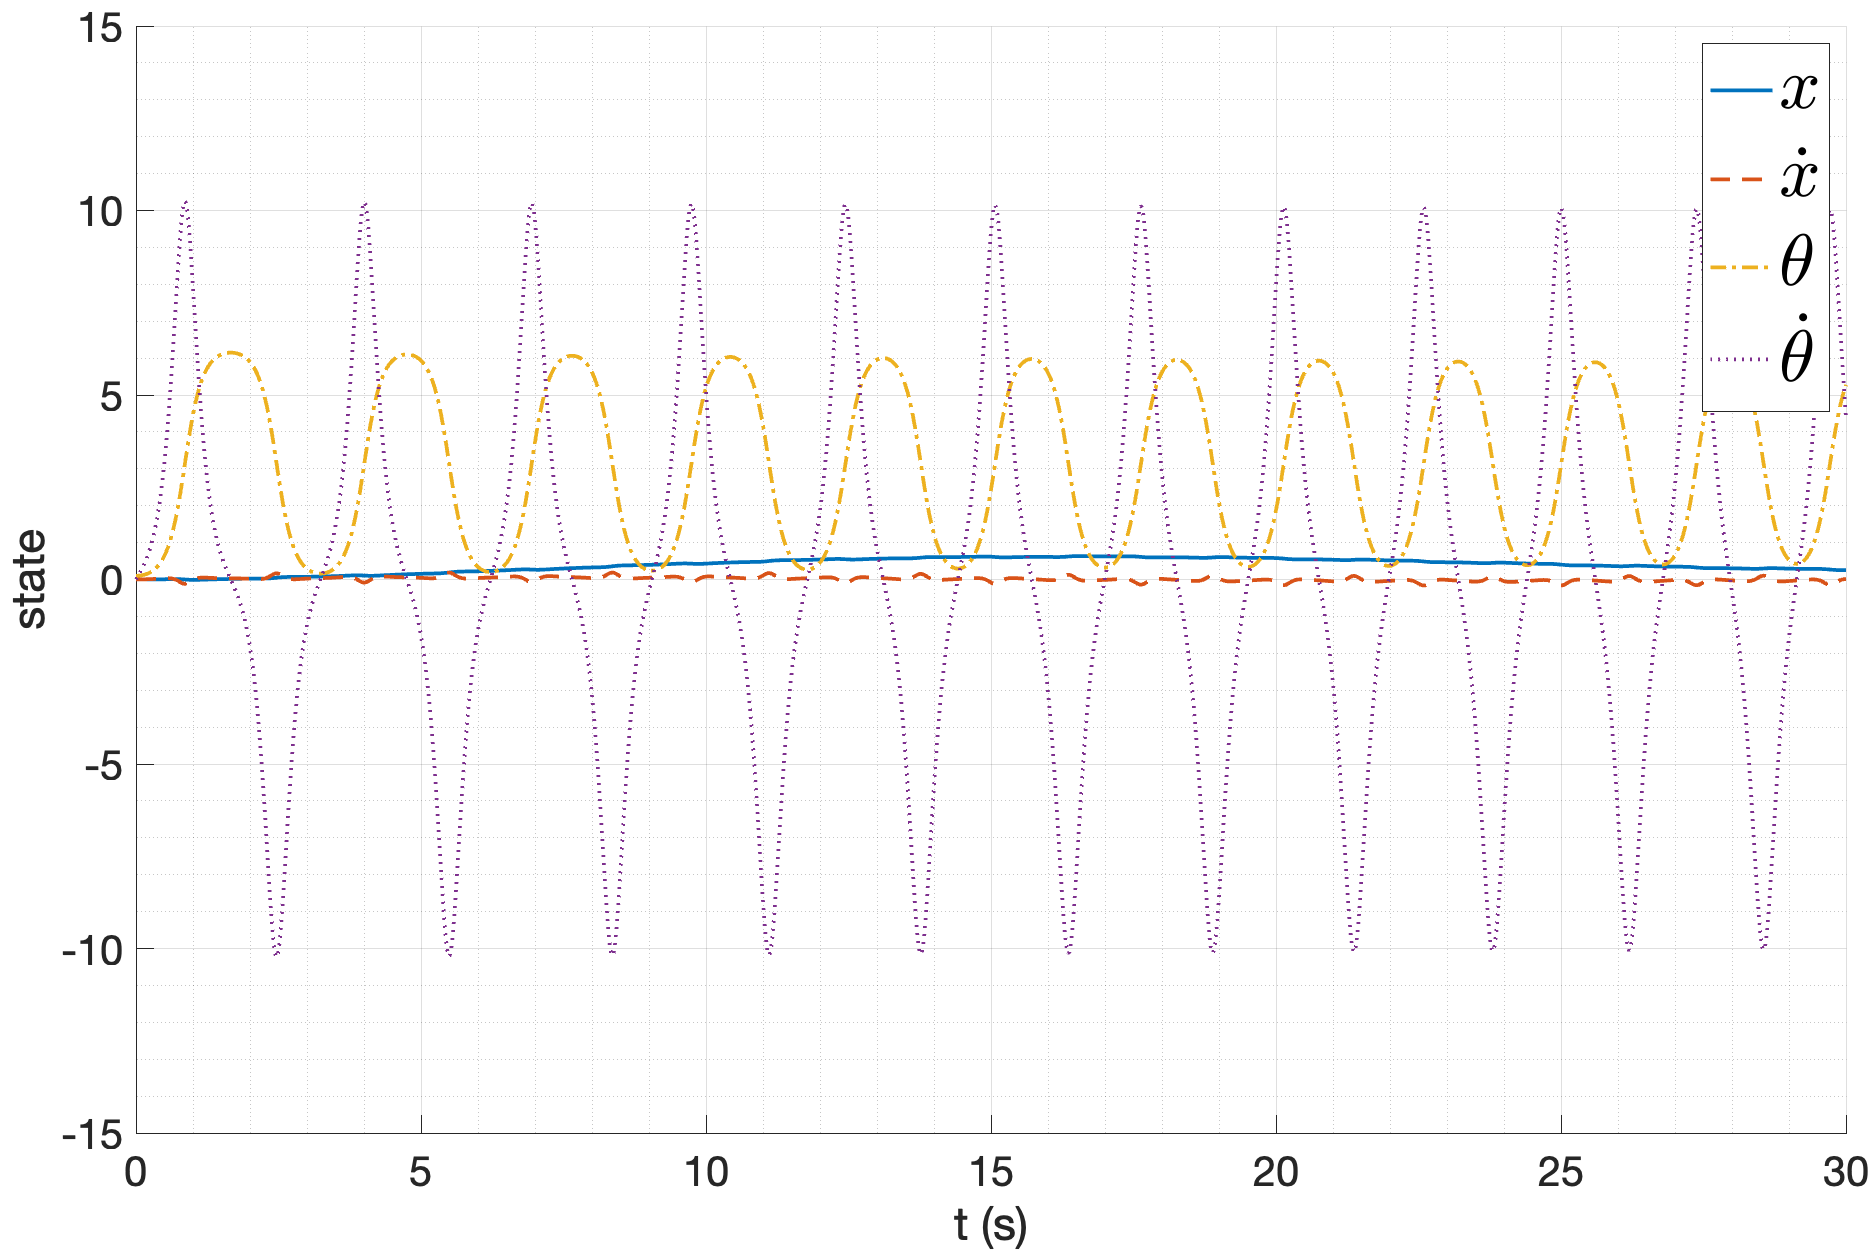
\includegraphics[width=\textwidth]{media/plots/nonmodal_controlers_min/state_6.png}
    \caption{Вектор состояния при $\alpha = 1.0$}
    \label{fig:nonmodal_control_alpha_2_3_state}
\end{figure}
\FloatBarrier 

Видно, что при увеличении степени устойчивости система сходится быстрее, при этом 
максимальное отклонение от положения равновесия тоже уменьшается. 
Получить регулятор с $\alpha = 1.0$ не удалось. 

\subsection{Синтез наблюдателя}
Использую линейные матричные неравенства Ляпунова проведем синтез 
наблюдателя полной размерности $\hat{x} = A\hat{x} + Bu + L(\hat{y} - y)$: 
\begin{equation}
    A^TQ + QA + 2\alpha Q + C^T Y^T + YC \preceq 0, ~~~ L = Q^{-1}Y, ~~~ Q \succ 0
\end{equation}
Решая данное неравенство для $\alpha = 3$ получаем матрицу наблюдателя: 
\begin{equation}
   L_1 = \begin{bmatrix}
    -10.33  & 0.06 \\ 
    -44.18  & -0.40 \\ 
    -0.15  & -13.19 \\ 
    -0.85  & -77.03 \\ 
    \end{bmatrix}
\end{equation}
Проверим устойчивость наблюдателя, найдя собственные числа системы $(A + L_1C)$: 
\begin{equation}
    \sigma(A - L_1C) = \begin{bmatrix}
        -5.17 + 4.18j \\ 
        -5.17 - 4.18j \\ 
        -6.59 + 3.74j \\ 
        -6.59 - 3.74j \\ 
    \end{bmatrix}
\end{equation}
По собственным числам видно, что наблюдатель устойчив, степень устойчивости равна $5.17$, что больше, чем заданное значение $\alpha = 3$. 

Для дальнейшего исследования проведем синтез еще одного наблюдателя $L_2$ со степенью устойчивости $\alpha = 10$.
Решая неравенство Ляпунова для $\alpha = 10$ получаем матрицу наблюдателя:
\begin{equation}
    L_2 = \begin{bmatrix}
    -31.54  & -0.07 \\ 
    -422.53  & -1.54 \\ 
    -0.17  & -33.90 \\ 
    -2.48  & -401.44 \\
    \end{bmatrix}
\end{equation}
Проверим устойчивость наблюдателя, найдя собственные числа системы $(A + L_2C)$:
\begin{equation}
    \sigma(A - L_2C) = \begin{bmatrix}
    -15.77 + 13.18j \\ 
    -15.77 - 13.18j \\ 
    -16.95 + 9.72j \\ 
    -16.95 - 9.72j \\
    \end{bmatrix}
\end{equation}
Желаемая степень устойчивости так же достигнута. Можно делать вывод о корректности синтеза наблюдателя. 

\subsection{Управление по выходу}
Рассмотрим управление системой, когда к измерению доступны только выходные переменные. Для этого будем использовать
наблюдатель и регулятор, полученные ранее (через матричные неравенства Ляпунова).

Возьмем два регулятора с различными степенями устойчивости $\alpha = 3$ и $\alpha = 10$: 
\begin{equation}
    \begin{array}{cc}
        K_1 = \begin{bmatrix}
        18189.83  & 11279.39  & -35086.93  & -8004.31 \\ 
        \end{bmatrix}  \\ 
        K_2 = \begin{bmatrix}
        1166417.18  & 245556.29  & -784739.34  & -132290.09 \\ 
        \end{bmatrix}
    \end{array}
\end{equation}
И два наблюдателя с различными степенями устойчивости $\alpha = 3$ и $\alpha = 10$:
\begin{equation}
    \begin{array}{cc}
        L_1 = \begin{bmatrix}
        -10.33  & 0.06 \\ 
        -44.18  & -0.40 \\ 
        -0.15  & -13.19 \\ 
        -0.85  & -77.03 \\ 
        \end{bmatrix} \\[3em]
        L_2 = \begin{bmatrix}
        -31.54  & -0.07 \\ 
        -422.53  & -1.54 \\ 
        -0.17  & -33.90 \\ 
        -2.48  & -401.44 \\ 
        \end{bmatrix}
    \end{array}
\end{equation}

Проведем моделирование систем с парами регуляторов и наблюдателей $(K_1, L_1)$, $(K_2, L_1)$ и $(K_2, L_2)$. Схема моделирования 
представлена на рисунке \ref{fig:KL_scheme}. 
\begin{figure}[ht!]
    \centering
    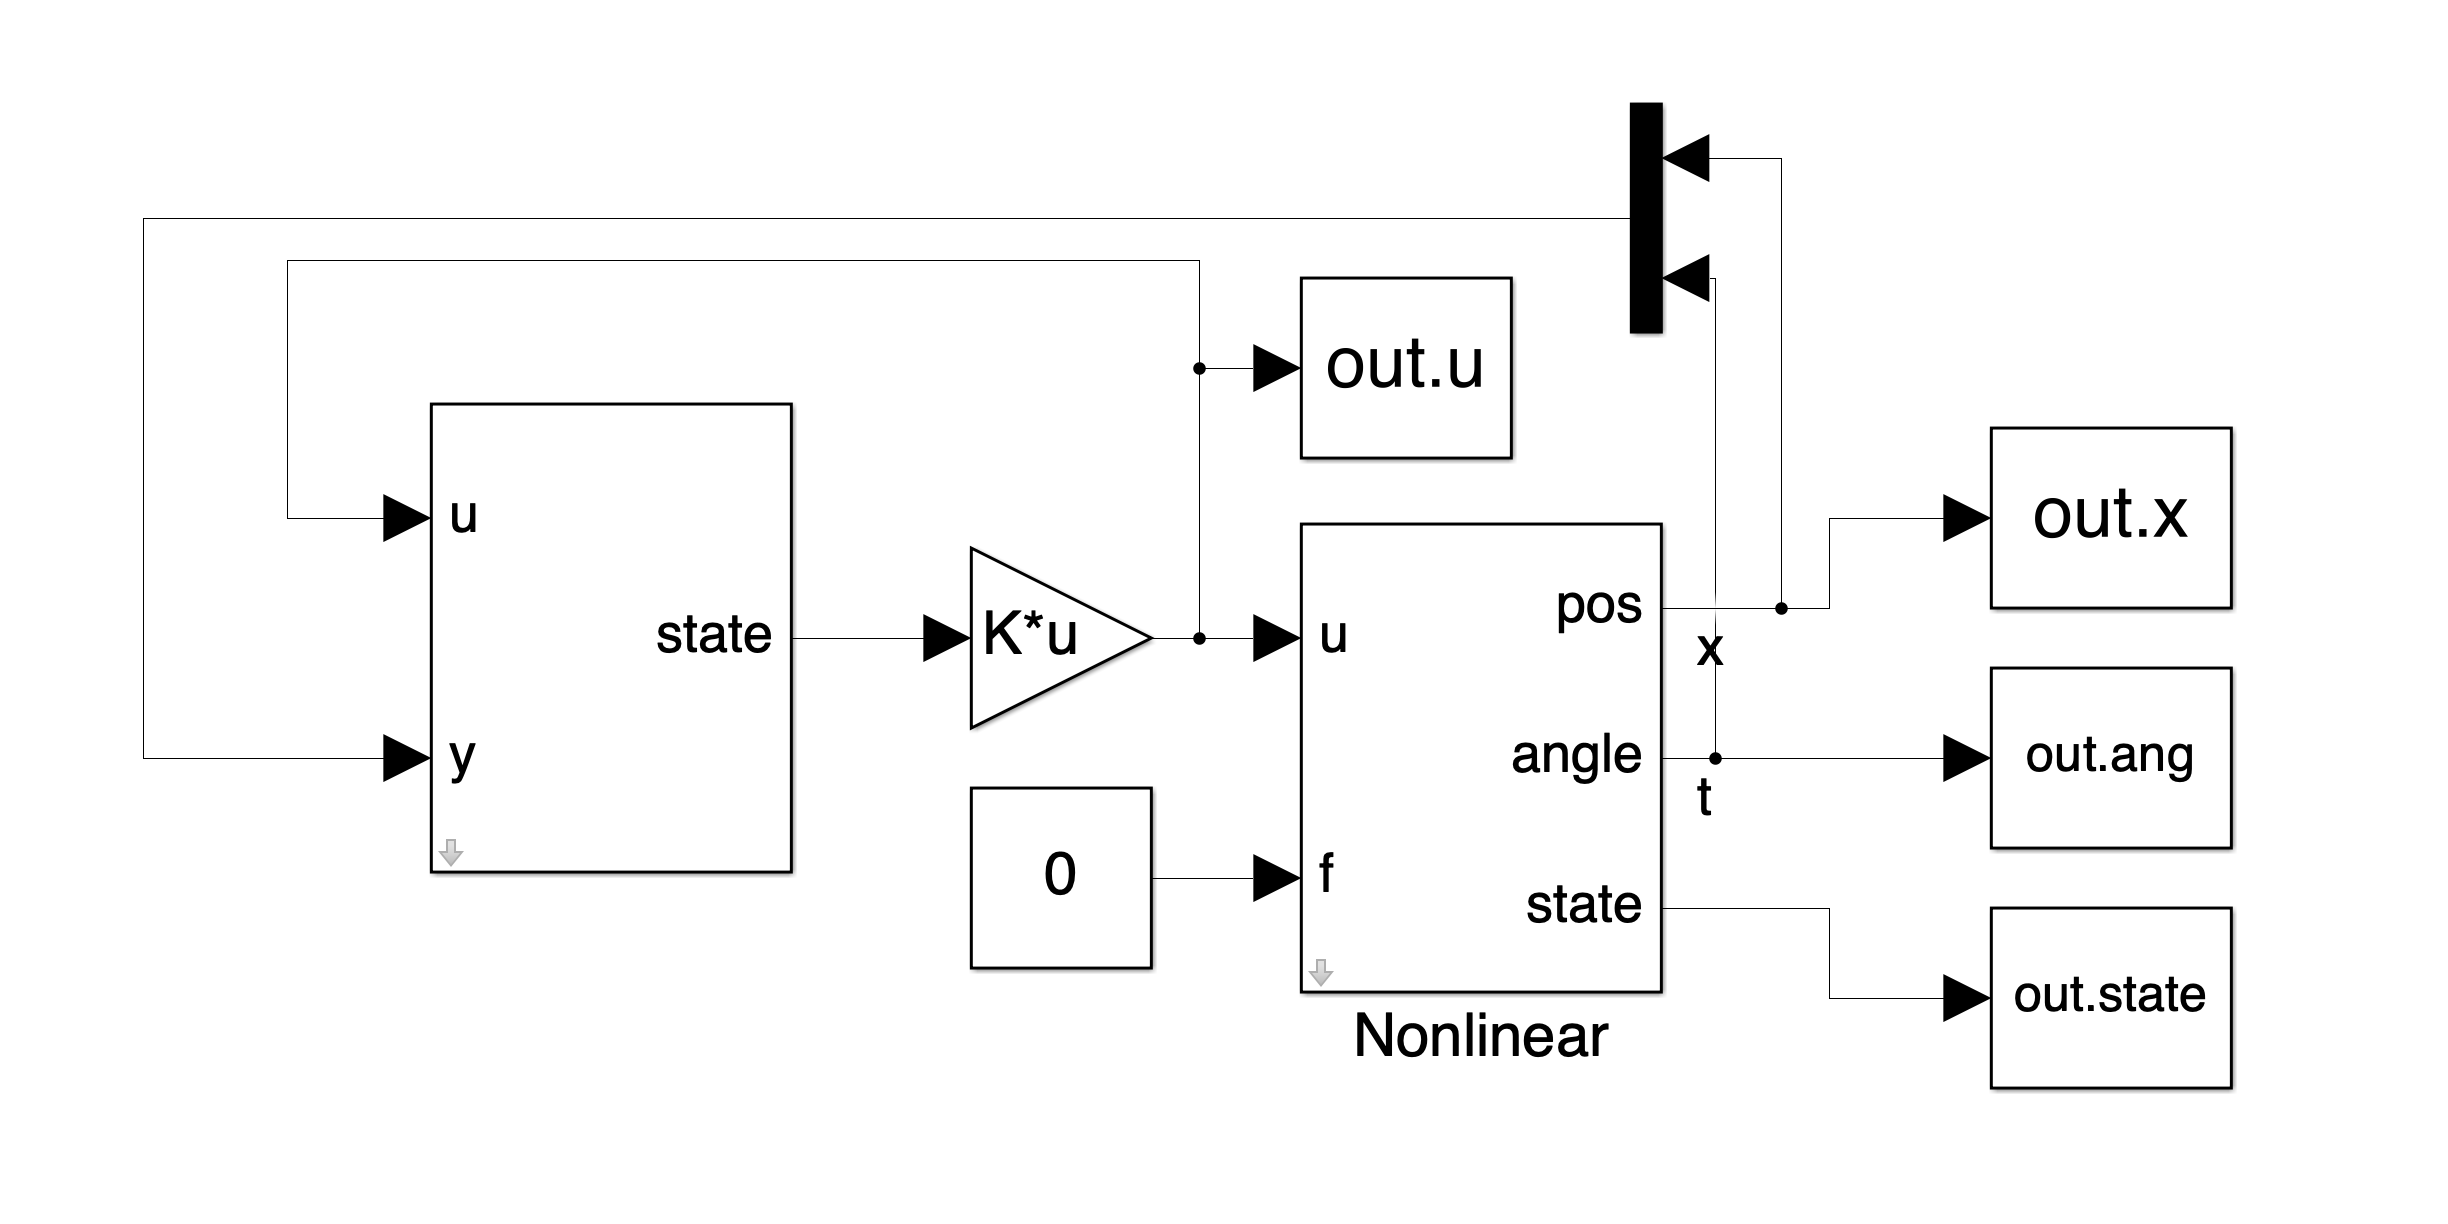
\includegraphics[width=0.8\textwidth]{media/KL_scheme.png}
    \caption{Схема моделирования системы с регулятором и наблюдателем}
    \label{fig:KL_scheme}   
\end{figure}
В качестве начальных условий возьмем $e_0 = \begin{bmatrix} 0 & 0 & 0 & 0 \end{bmatrix}^T$ для наблюдателя
и $x_0 = \begin{bmatrix} 0 & 0 & 0.2 & 0 \end{bmatrix}^T$ для системы. 

Результаты моделирования для пары $(K_1, L_1)$ приведены на рисунках \ref{fig:KL_1_out} - \ref{fig:KL_1_err}. 
\begin{figure}[ht!]
    \centering
    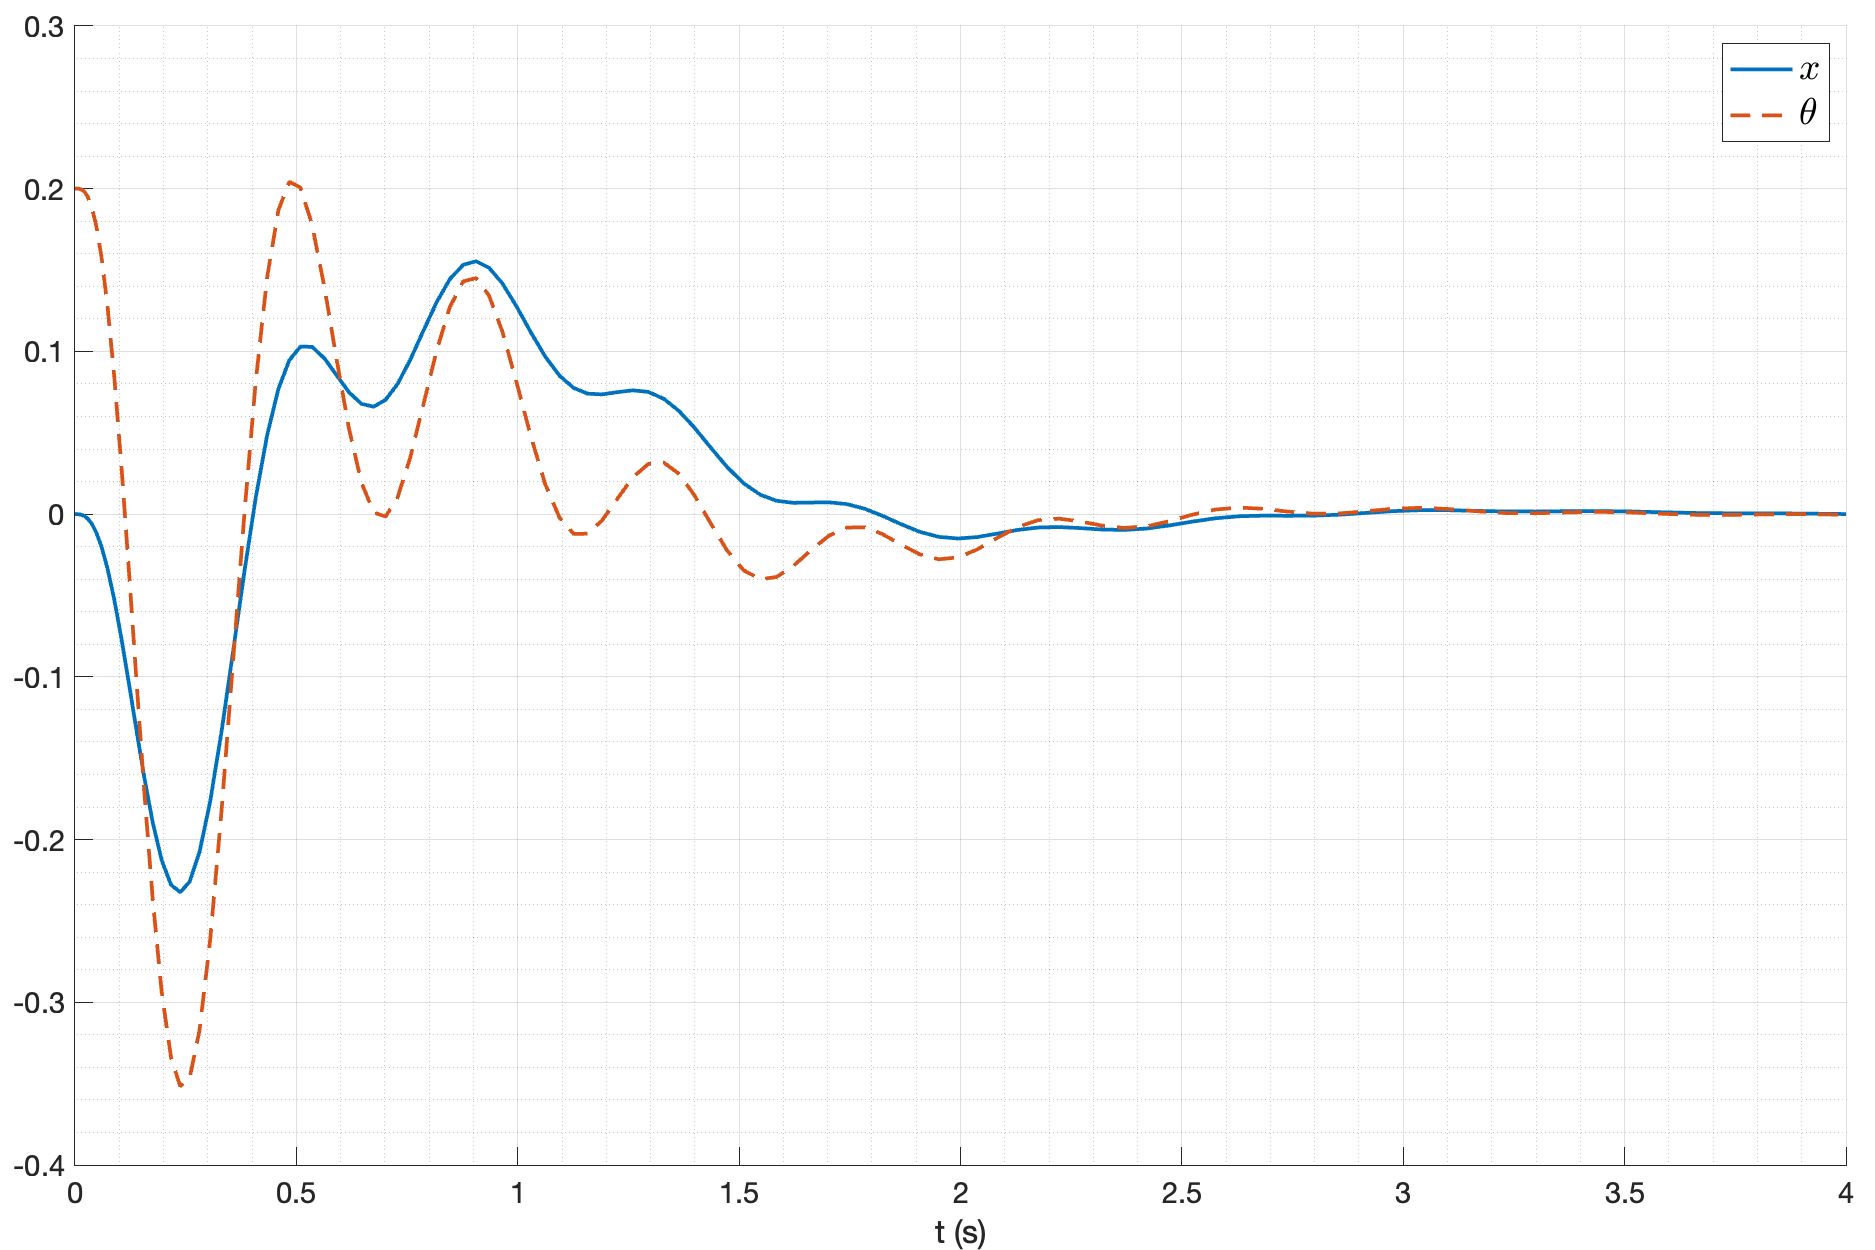
\includegraphics[width=\textwidth]{media/plots/nonmodal_observer_controller/kl_1.png}
    \caption{Переходный процесс при $(K_1, L_1)$}
    \label{fig:KL_1_out}
\end{figure}
\begin{figure}[ht!]
    \centering
    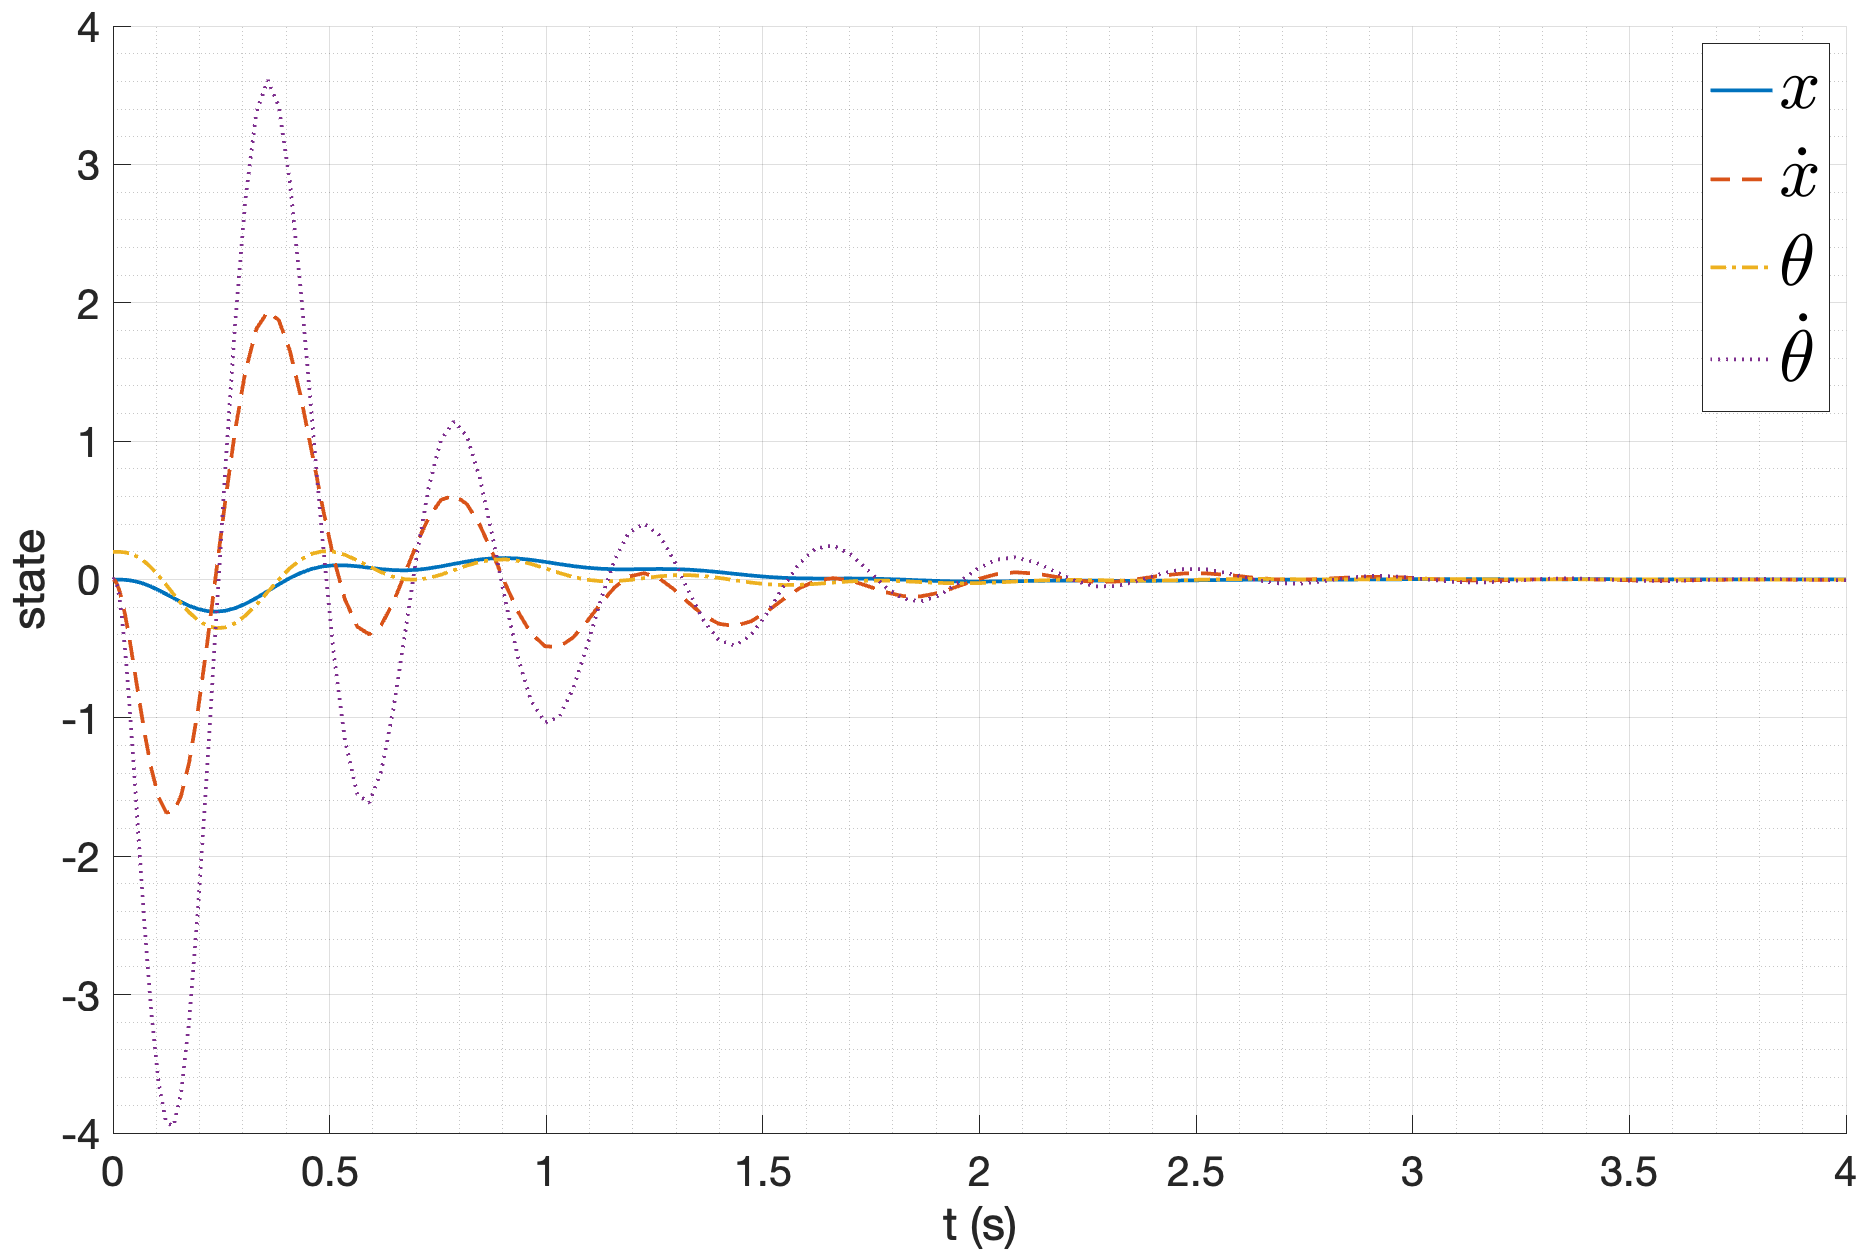
\includegraphics[width=\textwidth]{media/plots/nonmodal_observer_controller/state_1.png}
    \caption{Вектор состояния при $(K_1, L_1)$}
    \label{fig:KL_1_state}
\end{figure}
\begin{figure}[ht!]
    \centering
    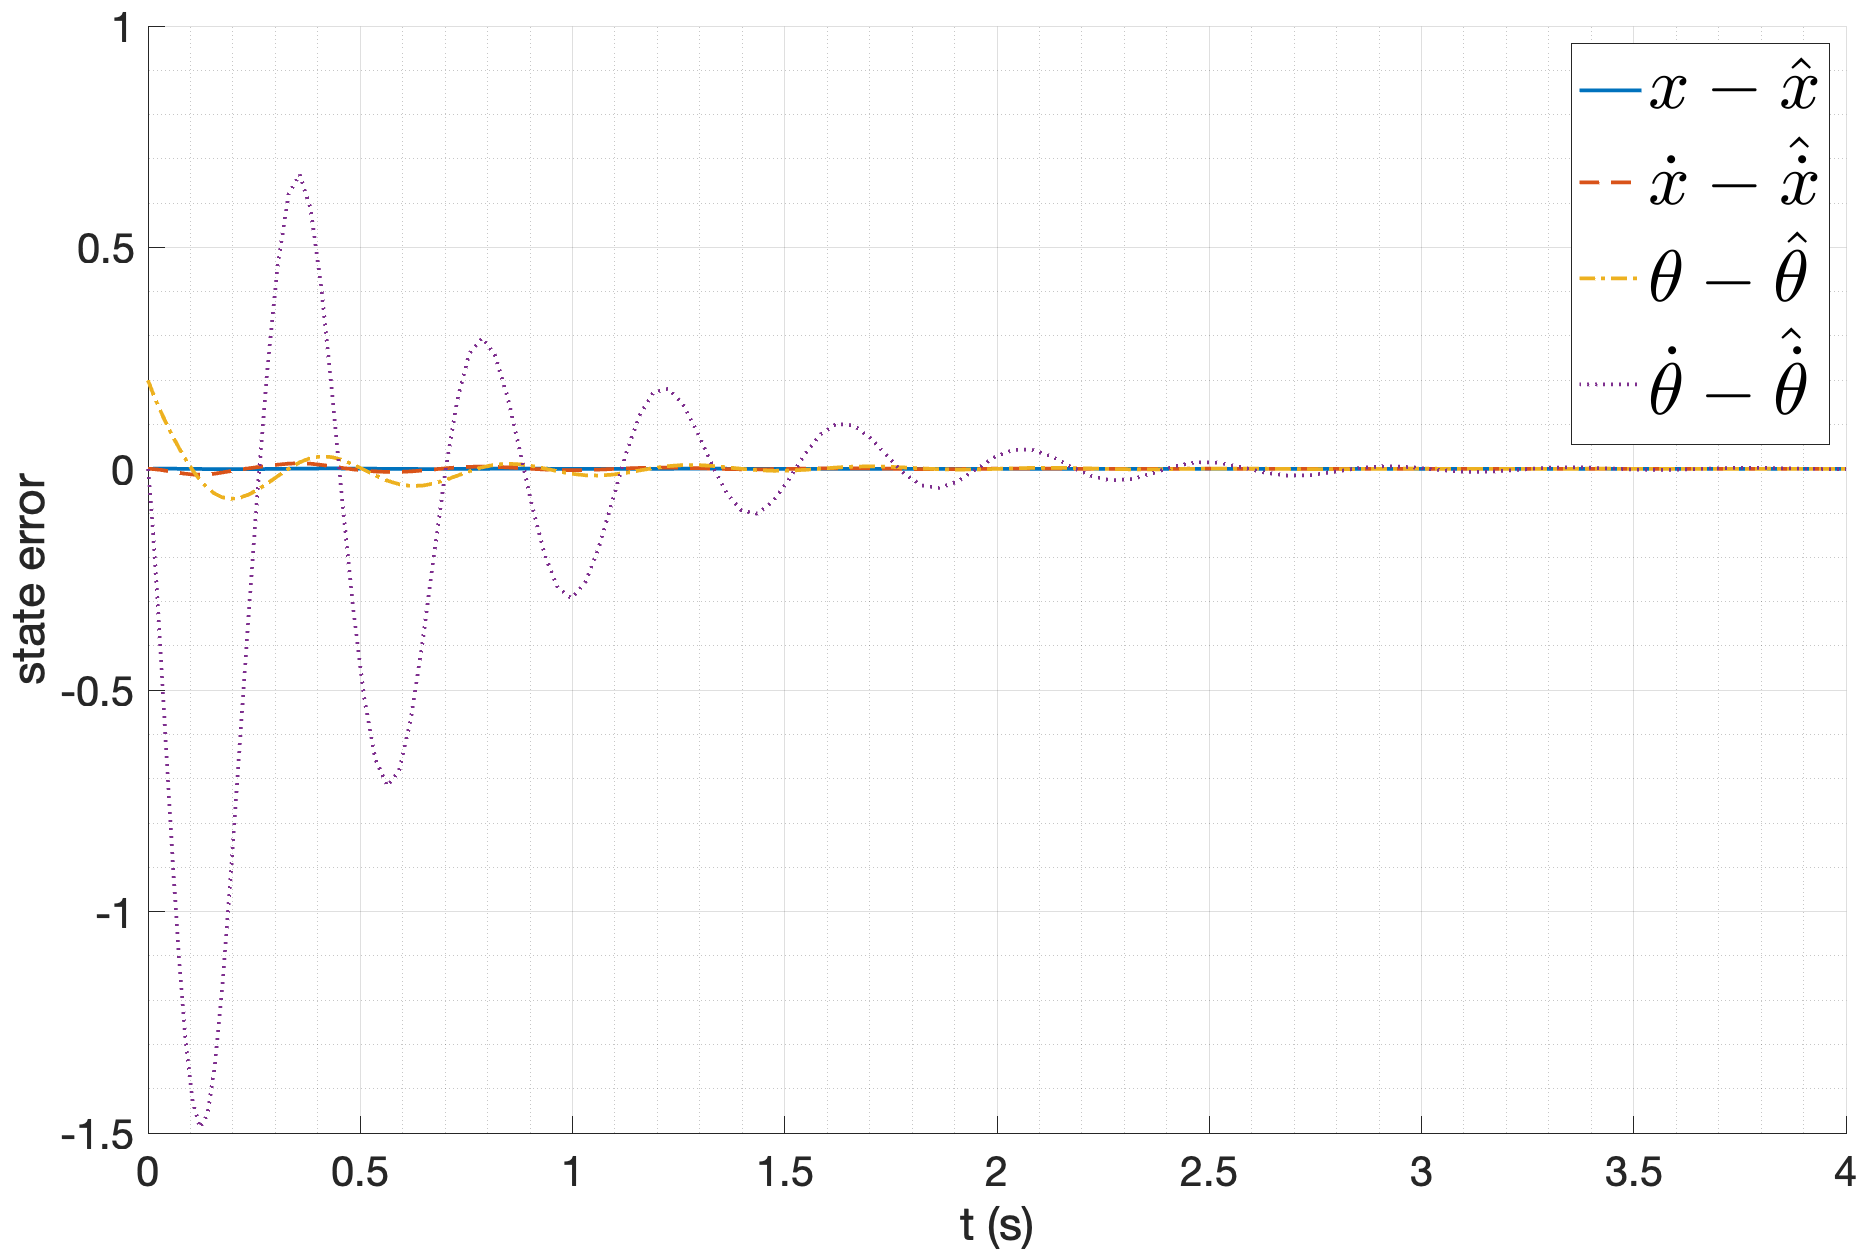
\includegraphics[width=\textwidth]{media/plots/nonmodal_observer_controller/kl_err_1.png}
    \caption{Ошибка наблюдения при $(K_1, L_1)$}
    \label{fig:KL_1_err}
\end{figure}
\FloatBarrier

Результаты моделирования для пары $(K_2, L_1)$ приведены на рисунках \ref{fig:KL_2_out} - \ref{fig:KL_2_err}.
\begin{figure}[ht!]
    \centering
    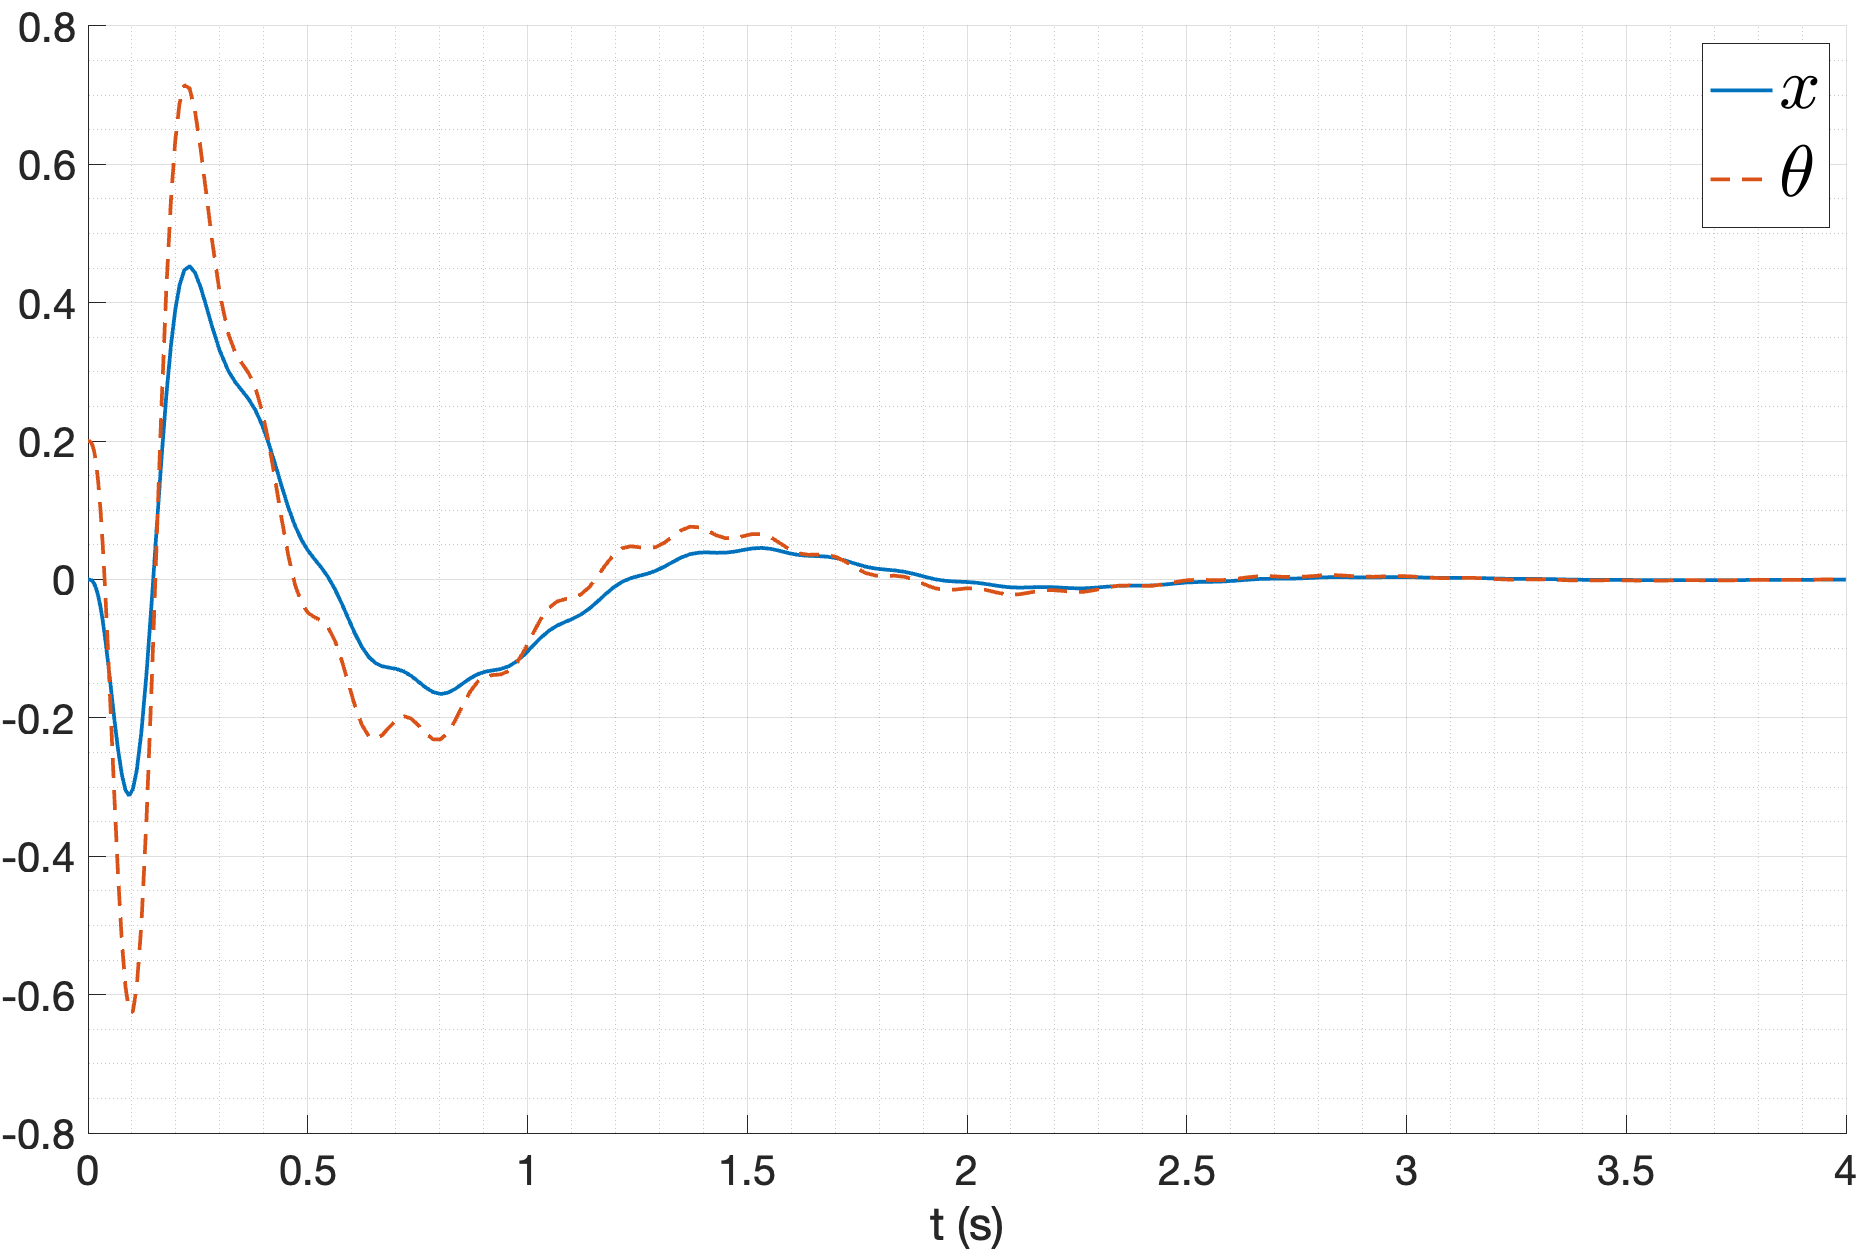
\includegraphics[width=\textwidth]{media/plots/nonmodal_observer_controller/kl_2.png}
    \caption{Переходный процесс при $(K_2, L_1)$}
    \label{fig:KL_2_out}
\end{figure}
\begin{figure}[ht!]
    \centering
    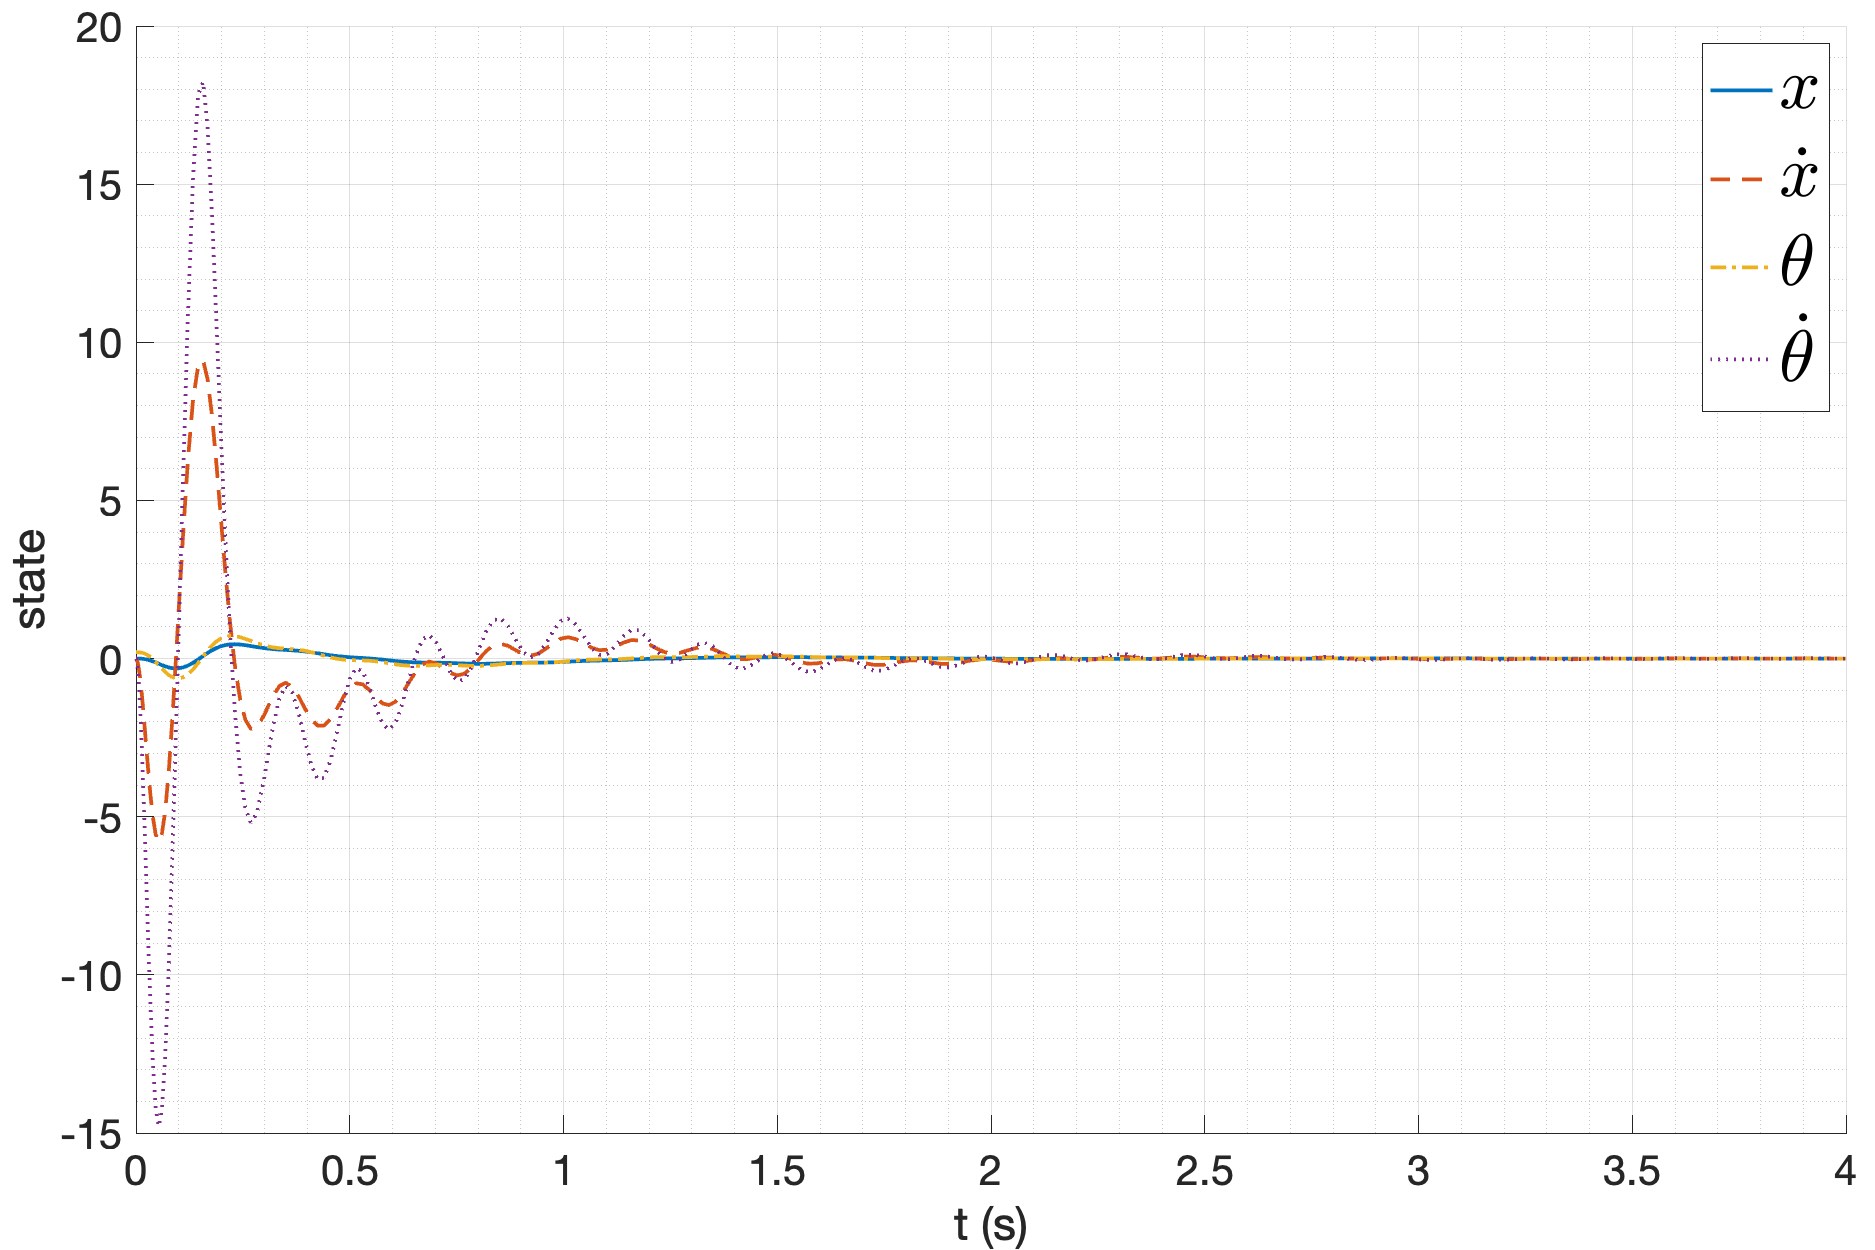
\includegraphics[width=\textwidth]{media/plots/nonmodal_observer_controller/state_2.png}
    \caption{Вектор состояния при $(K_2, L_1)$}
    \label{fig:KL_2_state}
\end{figure}
\begin{figure}[ht!]
    \centering
    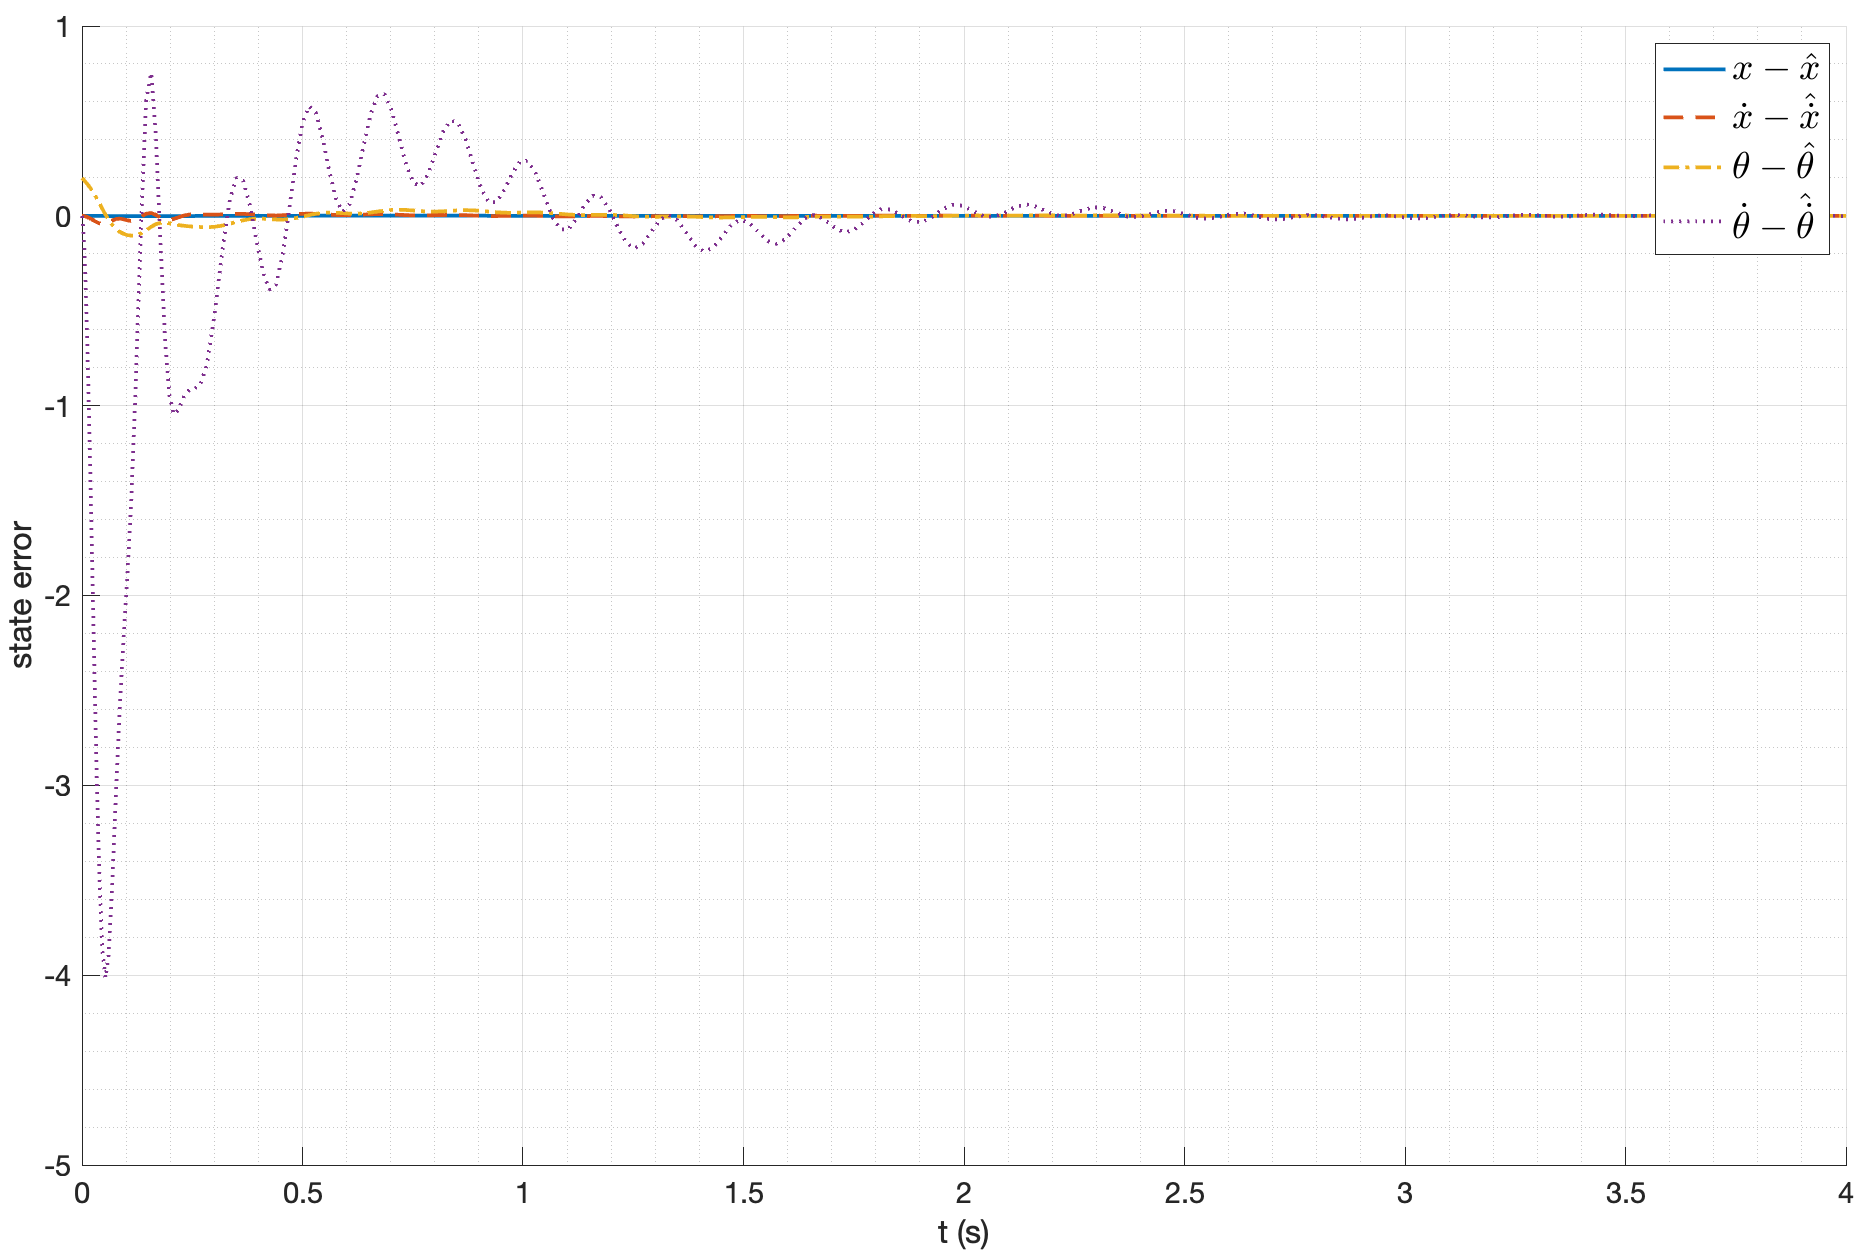
\includegraphics[width=\textwidth]{media/plots/nonmodal_observer_controller/kl_err_2.png}
    \caption{Ошибка наблюдения при $(K_2, L_1)$}
    \label{fig:KL_2_err}
\end{figure}
\FloatBarrier

Результаты моделирования для пары $(K_1, L_2)$ приведены на рисунках \ref{fig:KL_3_out} - \ref{fig:KL_3_err}.
\begin{figure}[ht!]
    \centering
    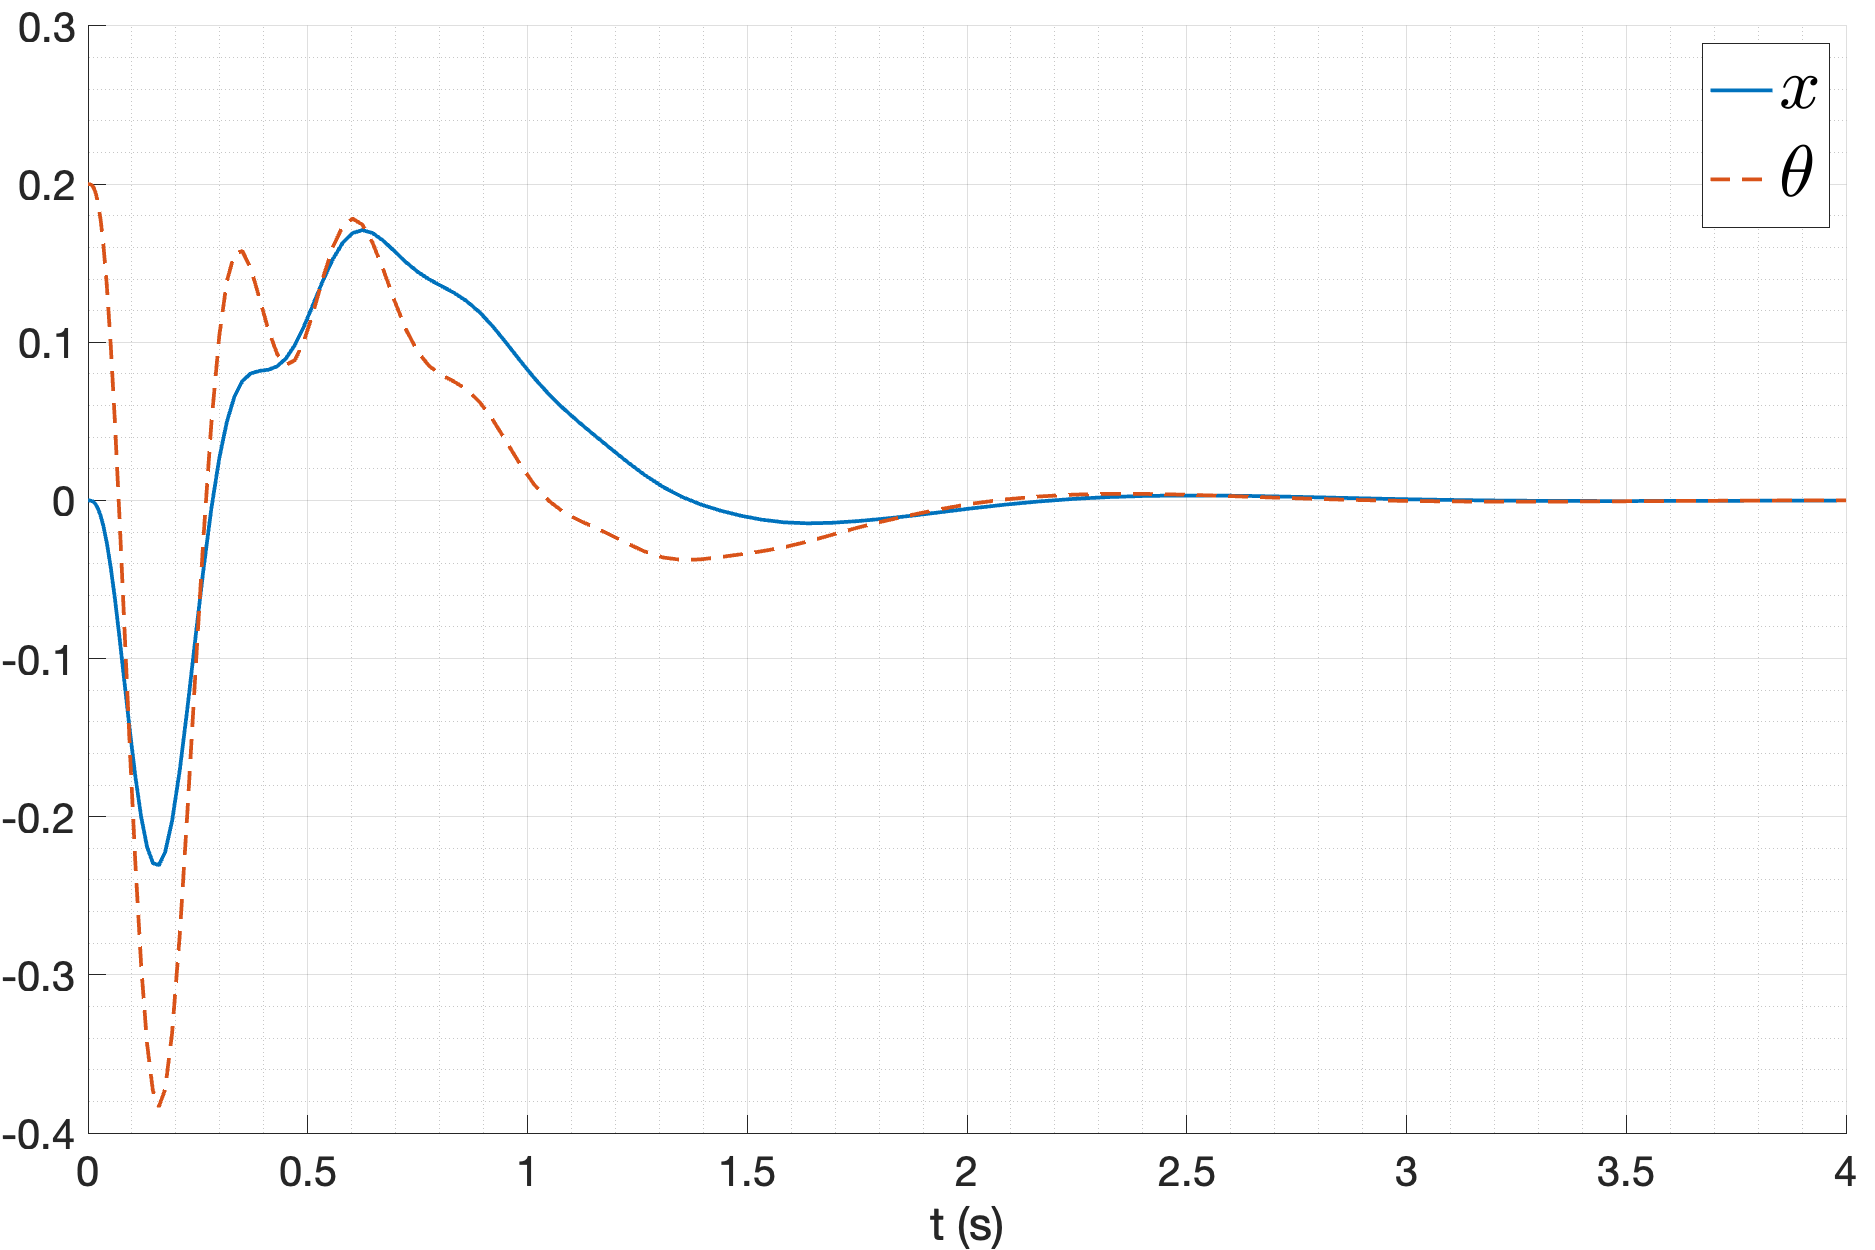
\includegraphics[width=\textwidth]{media/plots/nonmodal_observer_controller/kl_3.png}
    \caption{Переходный процесс при $(K_1, L_2)$}
    \label{fig:KL_3_out}
\end{figure}
\begin{figure}[ht!]
    \centering
    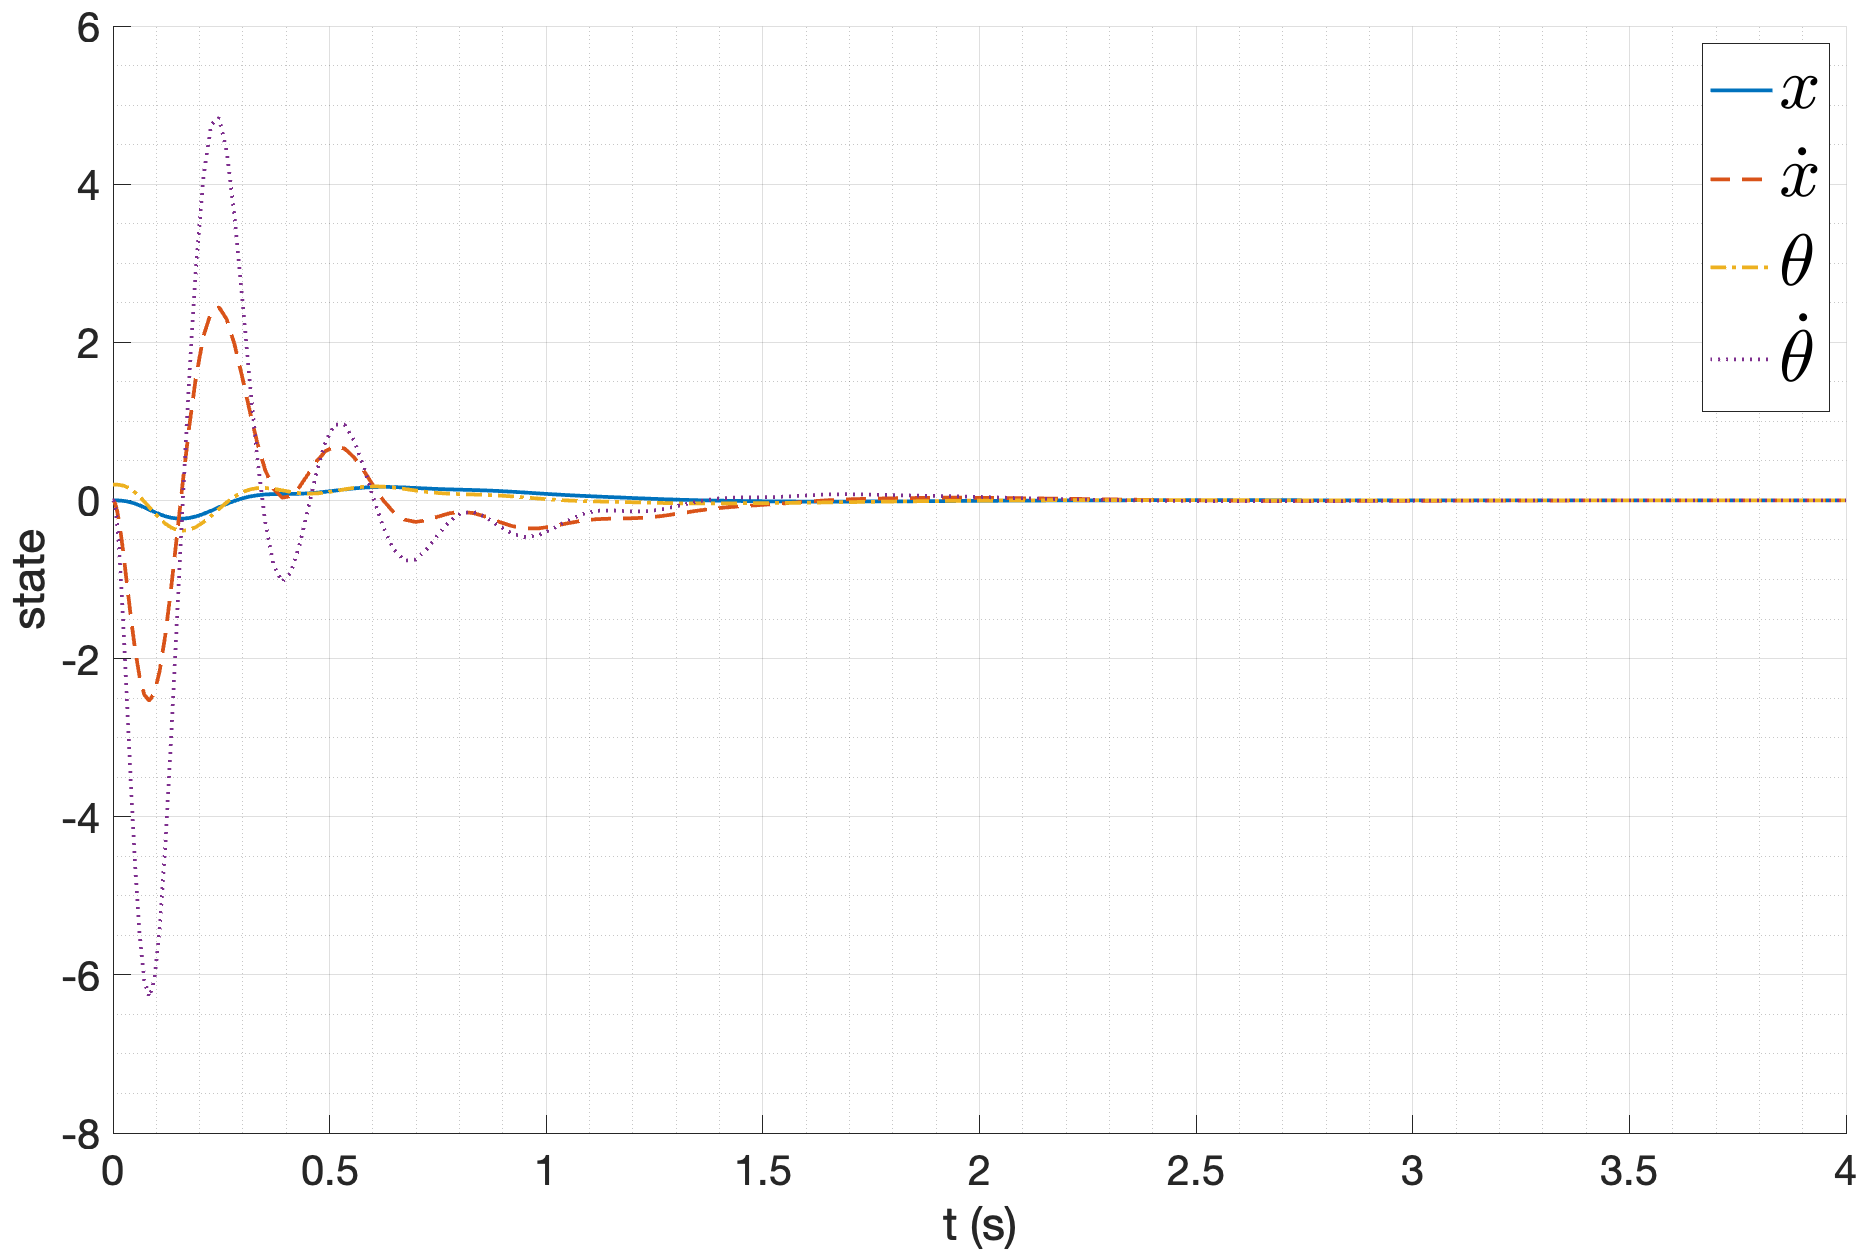
\includegraphics[width=\textwidth]{media/plots/nonmodal_observer_controller/state_3.png}
    \caption{Вектор состояния при $(K_1, L_2)$}
    \label{fig:KL_3_state}
\end{figure}
\begin{figure}[ht!]
    \centering
    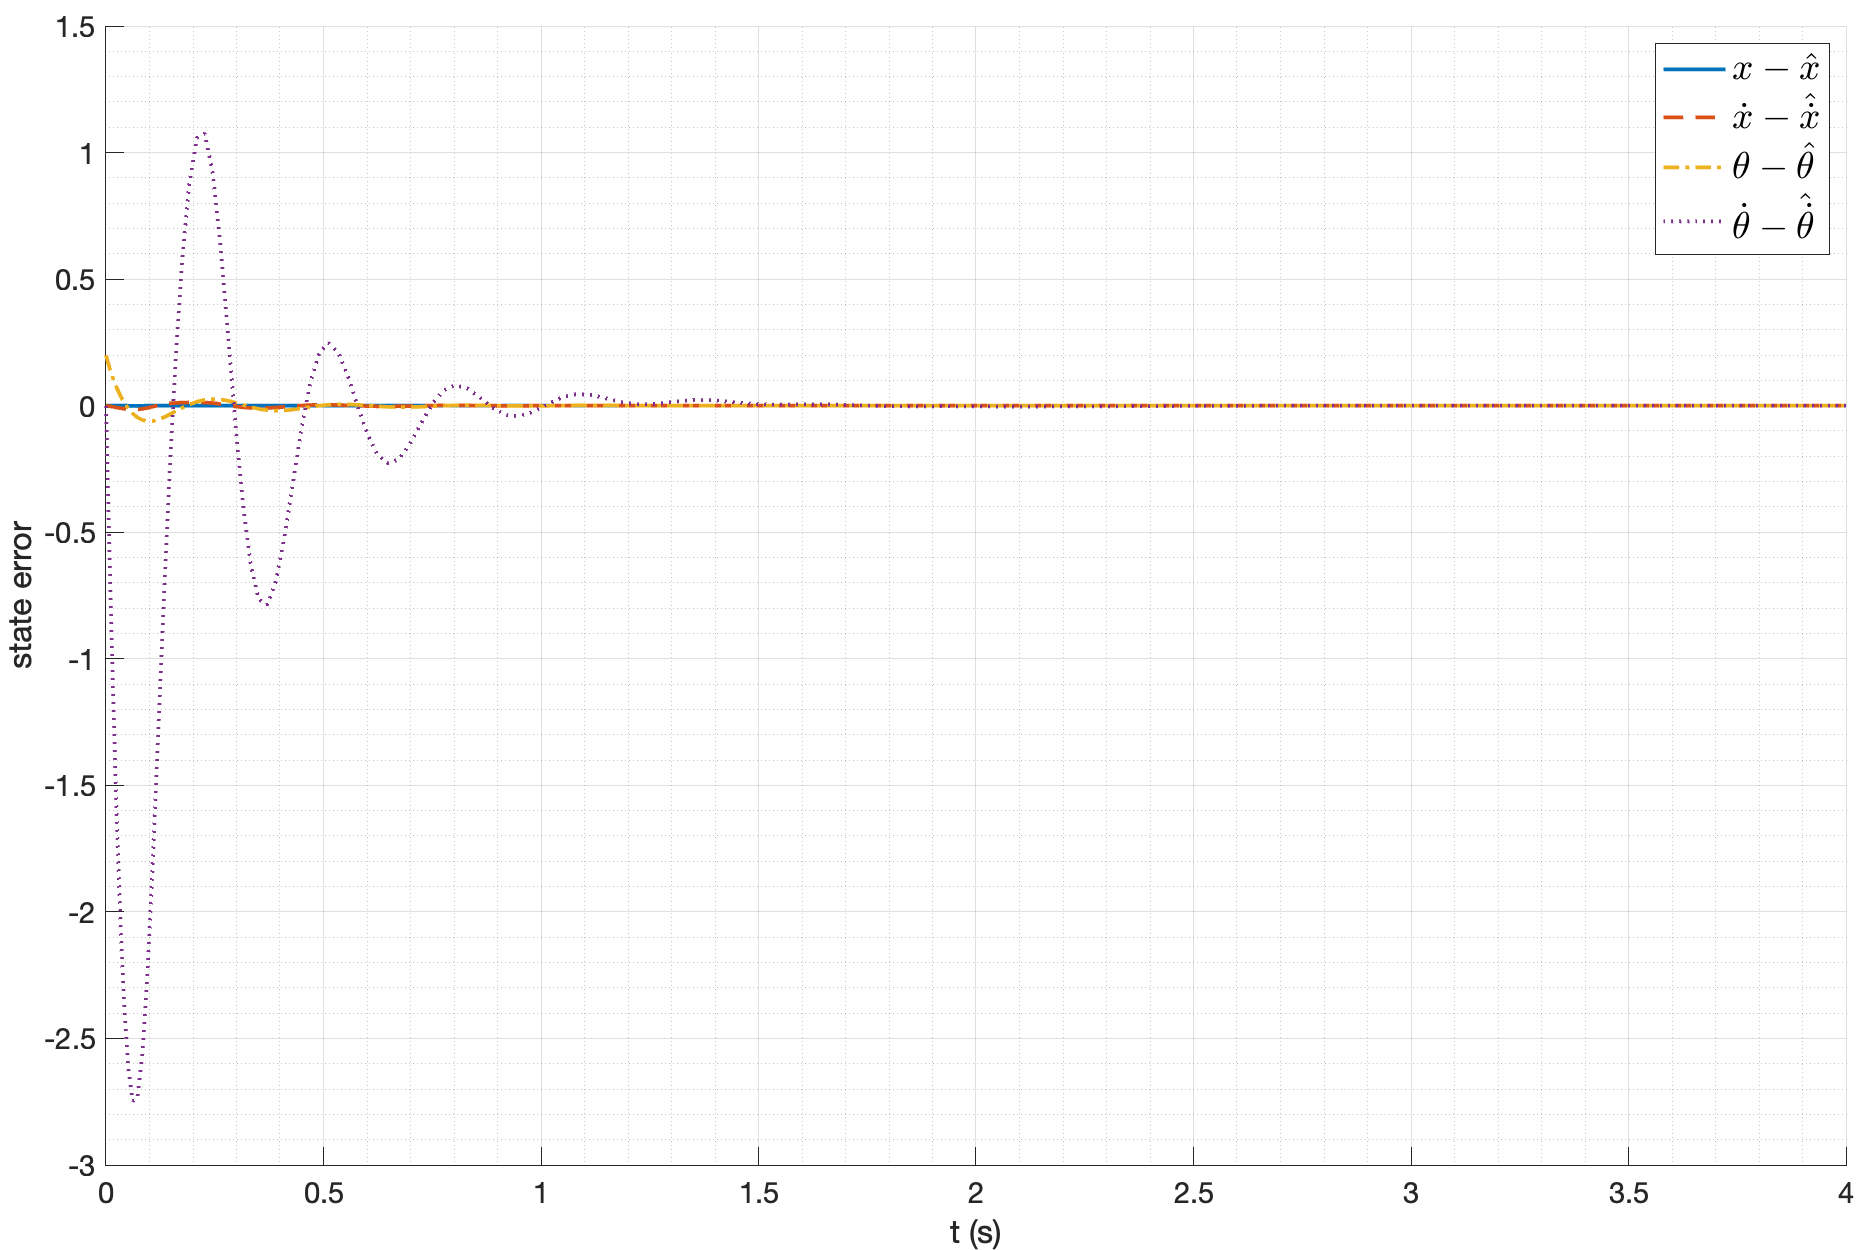
\includegraphics[width=\textwidth]{media/plots/nonmodal_observer_controller/kl_err_3.png}
    \caption{Ошибка наблюдения при $(K_1, L_2)$}
    \label{fig:KL_3_err}
\end{figure}

\FloatBarrier
По результатам исследования можно сделать вывод, что регулятор и наблюдатель вместе влияют на переходный процесс.
В первой паре, с \textit{слабым} регулятором и \textit{слабым} наблюдателем, система стабилизируется к положению равновесия
приблизительно за $3$ секунды, при этом ошибка наблюдения (для измерения угла отклонения маятника) приходит к нулю
за то же время. Во второй паре, с \textit{сильным} регулятором и \textit{слабым} наблюдателем, система стабилизируется
к положению равновесия приблизительно за $2.5$ секунды, при этом ошибка наблюдения также приходит к нулю за это же время, 
но ошибка наблюдения в начальный момент времени больше, чем в первой паре. В дальнейшем ошибка наблюдения становится 
примерно такой же, как и в первой паре. В третьей паре, с \textit{слабым} регулятором и \textit{сильным} наблюдателем,
система стабилизируется к положению равновесия приблизительно за $2.5$ секунды, при этом ошибка наблюдения
приходит к нулю за $1.5$ секунды, что меньше, чем в обоих предыдущих парах. 

Таким образом, можно сделать вывод, что при увеличении степени устойчивости как регулятора, так и наблюдателя,
система стабилизируется быстрее.

\subsection{Выводы}
В данной главе были рассмотрены немодальные методы синтеза регуляторов, которые позволяют задать степень устойчивости системы в целом.
Были синтезированы регуляторы с заданной степенью устойчивости, проведено исследование переходного процесса и управляющего воздействия при различных начальных условиях и степенях устойчивости.
Также были синтезированы регуляторы с ограничением на управление, позволяющие минимизировать управляющее воздействие.
Было рассмотрено управление системой по выходу, когда неизмеряемые состояния системы восстанавливаются с помощью наблюдателя. 
Это может быть полезно в реальных системах, где не все состояния могут быть измерены напрямую. 
